\documentclass[12pt]{amsbook}
\usepackage[utf8]{inputenc}
\usepackage{lmodern}
\usepackage[english]{babel}
\usepackage{fourier}
\usepackage[protrusion=true,expansion=true]{microtype}
\usepackage{amsmath,amsfonts,amsthm,amssymb,amscd}
\usepackage{gensymb}
\usepackage[final=true]{hyperref}
\def\UrlBreaks{\do\/\do-}
\usepackage[pdftex]{graphicx}
\usepackage{xspace}		
\usepackage[svgnames]{xcolor}	
\usepackage{fancyvrb}
\usepackage{fancyhdr}
\usepackage{algorithmic}
\usepackage{float}
\usepackage{wrapfig}

\pagestyle{fancyplain}
\fancyhead[LE,RO]{\slshape\thepage}
\fancyhead[RE]{\slshape \leftmark}
\fancyhead[LO]{\slshape \rightmark}
\fancyfoot[L]{\small \url{http://toddvance.tech}}		
\fancyfoot[C]{\raisebox{-10pt}{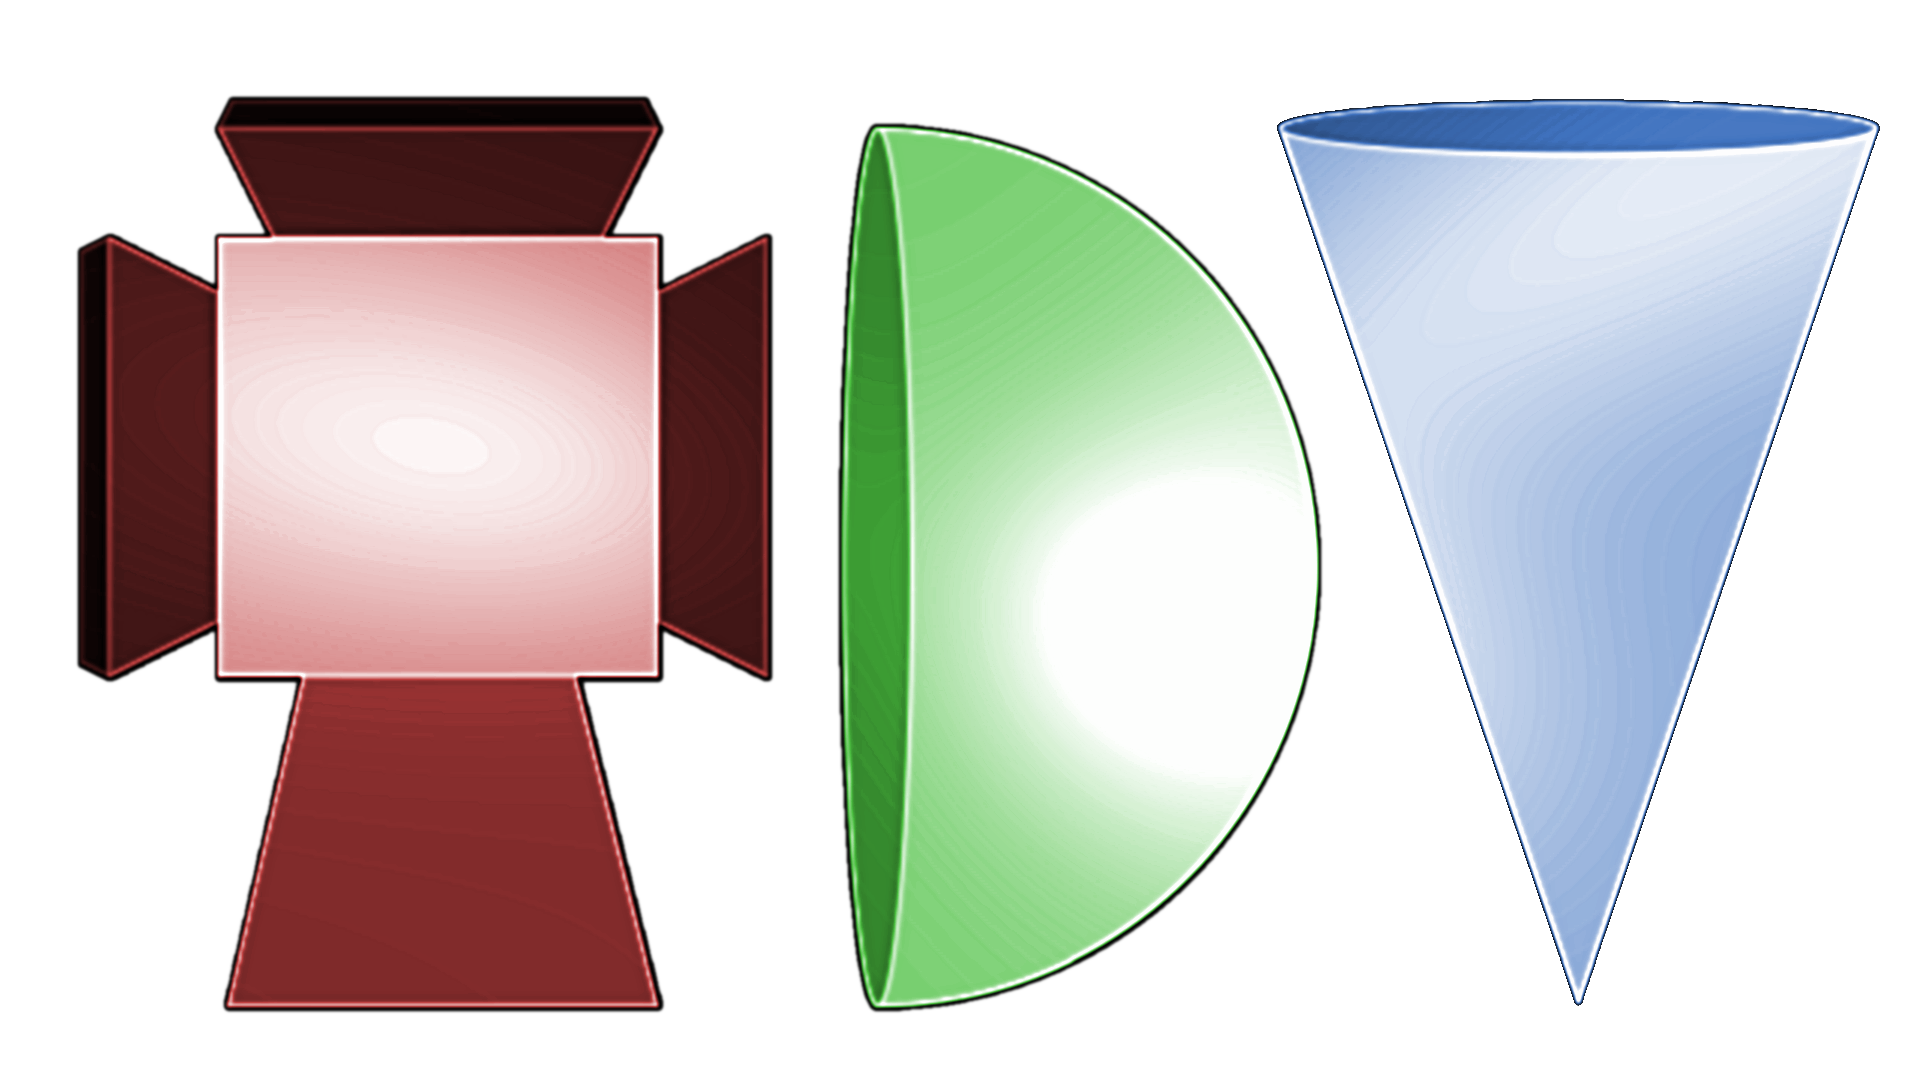
\includegraphics[width=0.5in]{monogram-transparent.png}}}											
\fancyfoot[R]{}								
\renewcommand{\headrulewidth}{0pt}			
\renewcommand{\footrulewidth}{0pt}
\setlength{\headheight}{13.6pt}
\newcommand{\horrule}[1]{\rule{\linewidth}{#1}} 	% Horizontal rule


%theorem styles

\newtheorem{theorem}{Theorem}[chapter]
\newtheorem{lemma}[theorem]{Lemma}

\theoremstyle{definition}
\newtheorem{definition}{Definition}[chapter]
\newtheorem{exercise}{Exercise}[chapter]
\newtheorem{task}[exercise]{Task}
\newtheorem{preview}[exercise]{Preview}
\newtheorem{review}[exercise]{Review}
\newtheorem{challenge}[exercise]{Challenge}
\newtheorem{project}[exercise]{Project}


\theoremstyle{remark}
\newtheorem{remark}[theorem]{Remark}

\numberwithin{figure}{chapter}
\numberwithin{table}{chapter}
\numberwithin{section}{chapter}
\numberwithin{equation}{section}

%Title, Author, and date

\title{Rat Race: Creating a 2D Classic Arcade Style Maze Chase Game in Unity3D}
\author{Todd D. Vance}
\address{Deplorable Mountaineer}
\email{support@toddvance.tech}
\date{\today}

%\subjclass[2010]{Primary }

\keywords{game, csharp, unity, arcade, PCG, AI}

%additional commands

\newcommand{\csharp}{\ensuremath{\mbox{C}\#}\xspace}
\newcommand{\astar}{\ensuremath{\mbox{A}*}\xspace}
\newcommand{\abs}[1]{\lvert#1\rvert}

\makeindex
\begin{document}
\frontmatter
\begin{abstract}
\end{abstract}

\maketitle{}
\setcounter{page}{2}%adjust as needed to make TOC page correct
\setcounter{secnumdepth}{3}
\setcounter{tocdepth}{3}
\tableofcontents{}

%preface, etc.

\mainmatter
%%%%%%%%%%%%%% BEGIN DOCUMENT %%%%%%%%%%%%%%%

\chapter{Let's Create a Game!}
Remember the Golden Age of the arcade in the 1980s? It was a PacMan-eat-dot industry; any game that didn't earn a quarter every three minutes got removed and replaced.  Thus the games were built to have lights and sounds to attract the players, and then to challenge the players enough that they are likely to lose the game fast. Still, from time to time, a skillful player would do unusually well and achieve a spot on the high score list.

We can build a game of this type.  We have the technology: faster, stronger, better.  And it will cost much less than six million dollars.  We shall use the Unity game engine, whose game editor and integrated development environment (IDE) runs on the PC and Macintosh.  Unity can deploy games than run on the PC and Mac as well as on Linux, in a web browser and on mobile devices.


\begin{figure}[h]
  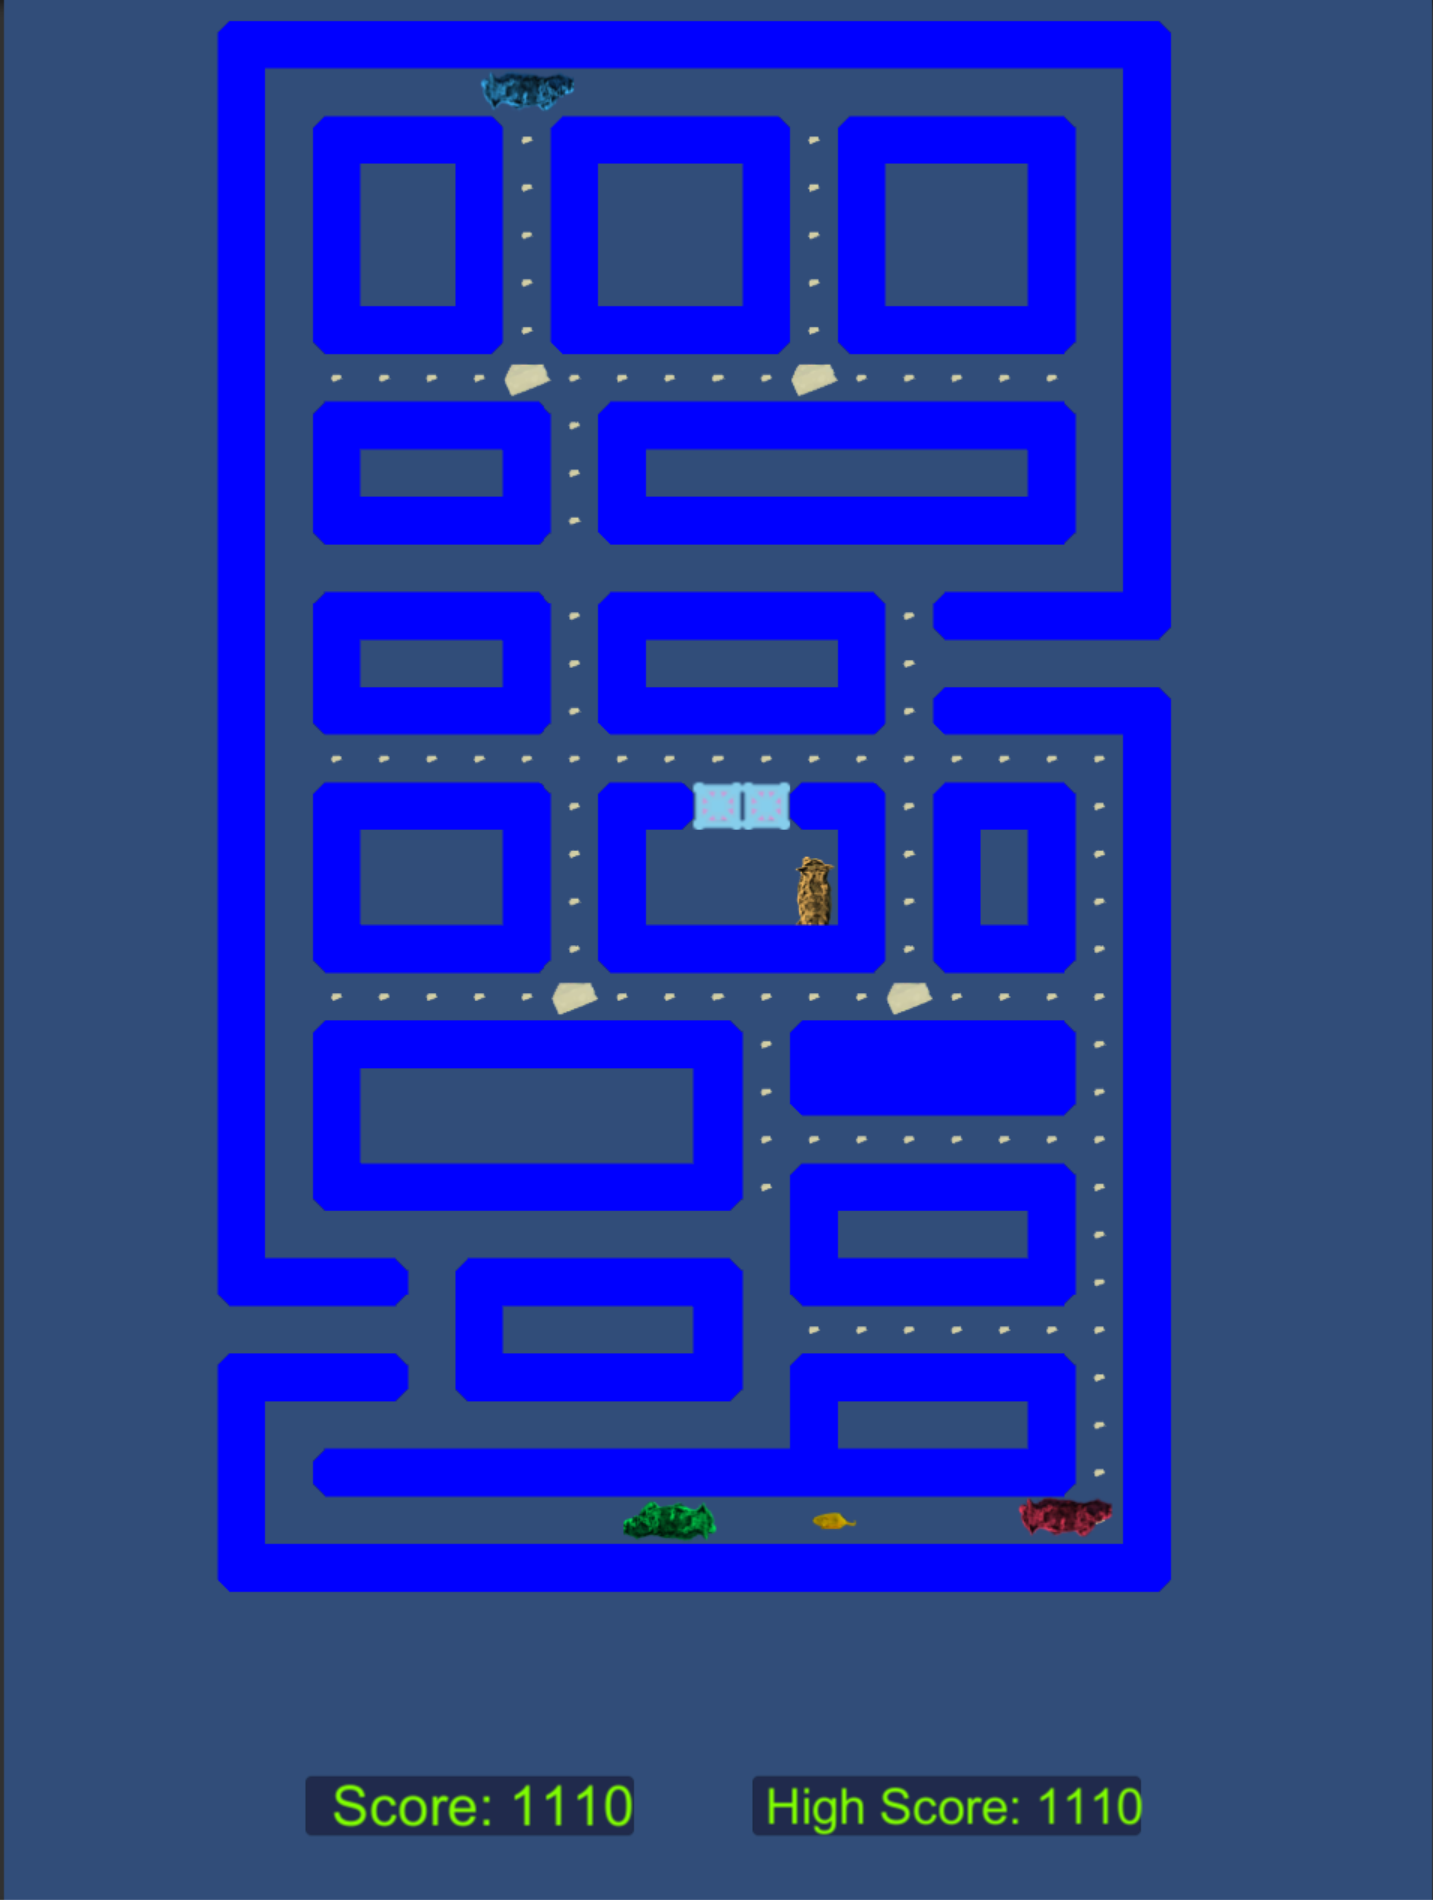
\includegraphics[width=3in]{ratrace.png}
  \caption{Placeholder concept screenshot of Rat Race}
  \label{fig:placeholder}
\end{figure}

Figure \ref{fig:placeholder} shows a screenshot of the game we shall create in this book.  The player controls a mouse sprite which must eat all the cheese in the maze without being eaten by some very aggressive AI-controlled cats.  Elements of this game and the process for creating it include:

\begin{itemize}
\item Installation of Unity and various game-making tools
\item Introduction to software tools for game making
\item Object-oriented \csharp programming
\item Introduction to Artificial Intelligence (AI) programming
\item Motion control for both the cats and the mouse
\item Grid-based automated level building and Procedural Content Generation (PCG)
\item Score keeping with high-score saving
\item Multiple lives
\item Teleportation tunnels
\item Sound and music and animated sprite assets
\item A game state system managing the title and high score screens
\item Cutscenes
\item Source control
\item Refactoring
\item Design patterns
\item Pseudocoding algorithms
\item Designing an algorithm to produce a specific result
\item Making the game work on multiple platforms
\item Publishing your game for money or just for fame
\item And more....
\end{itemize}

This book can be treated as a course that covers many aspects of gameplay programming.  The first reading, carefully following all the steps, lets the reader build the Rat Race arcade game.  After that, it can be used as a reference for designing and building other 2D arcade-style games.

After this introduction, the course will properly begin with downloading and installing the main tool, Unity 3D (currently at version 5.6).  Other tools are either optional or can be replaced with alternatives.  Tools will be needed to create sound and sprite assets, in particular.  An alternative is to find and download assets from the web.  There are plenty of free and paid assets.  However, check licensing information carefully.  Some assets cannot be used commercially and must be avoided if you intend to sell the game.  Some cannot even be used in a game published for free.

Next, the game is prototyped, and then an overall design of the game is be considered along with implementation notes.  This includes the game mechanics (rules and how input is interpreted by the game) as well as the assets (artwork, including sound, images, and structure of levels),  game state (such as Attract Mode and leveling up), and architecture (how the software is structured to build the game). 
 
Then, the game building continues in a spiral fashion.

\section{Elements of a Classic Arcade Game}

Think back to a 1980s style stand-up arcade game.  When you entered the arcade, most games would be in what is called ``Attract Mode,'' intended to entice you to spend a quarter.  Typically they made no, or maybe a little bit of sound (the real sound began as a reward for spending the quarter) and the controls would be non-functional.  There would be a title screen with logos and graphics to announce the game.  After a few seconds, it would change to some other screen, perhaps a description screen giving the story of the game or maybe a quick how-to-play, perhaps showing various pickups and their point values.  

After several seconds, a high-score list would be shown.  The top ten scores with the initials of players promised fame (at least in the local community) and one's name on a TV screen (in those days before YouTube, a person's initials appearing on something that looked like a TV for others to see was magical, particularly to children).  This generated competition and caused people to play again and again, always trying to beat their own, and their friends' high scores. Children also had fantasies of ``real world glory'' from scoring well in video games too: Ender's Game \cite{Car94} and The Last Starfighter\cite{Fos84} (both of which are also movies) illustrated such fantasies.

Ultimately came the demo: essentially a video playback (without all the game sounds, or at least with a reduced number of sounds) of a game in progress to show how it can be done.  The playback did not usually last long before either the player died or it was just interrupted at an arbitrary point and the game returned to the title screen and cycled again.  (Later, when arcade games came to home computers, some games let users record their own demos to show to friends).

The game would continue cycling between these states while in Attract Mode, until someone inserted a quarter.  When that happened, there was typically some kind of sound (as well as a change to the text and/or graphics on the screen) to acknowledge the quarter, and a text bar somewhere on the screen would say ``1 credit'' or ``Credits: 1'' or similar.  Adding more quarters would add more credits.  Each credit represents one play, or for games that let two or more players play, each credit allows one additional player to play.  Some later games (toward the end of the Golden Age) let you trade credits for additional lives (or powerups) in a game.  This was controversial, since a person with more quarters to spend could boast a higher score without really having more skill.

If the player pressed the ``Start Game'' button, and the number of credits was positive, the number of credits would decrement and the game would begin.  One could also press the ``Start Two Player Game'' (or other buttons) and if there were enough credits, the appropriate number of credits would be subtracted and a multiplayer game would start.  The way multiplayer games worked were either two or more sets of controls, or one set of controls and players took turns between lives.

Then the game would start.  Typically there would be some kind of introduction music and animation, and then the game would begin for real.  In these games, the player had to hit the ground running.  If the player looked away for even a short time, the player would lose.  Remember, it was all about getting people to spend quarters.

What happened afterward was dependent on the game being played, but typically, the player would have some small number (three was common) of lives.  Each time the player died, he ``lost a life'', and the game was over when he had no more lives left.  If instead of dying he completed a level, he would advance to the next level.  There might be a cutscene (typically an animation and sound sequence that tells the next part of the story) or something as simple as the screen flashing or some level-up sound, something to reward the player for a job well done.  The next level would begin, and it would be harder than the last level.

Sometimes there would be bonus levels: typically, one couldn't die in that level, it was just a way to relax and add to the score.  This was a reward for completing a number of levels.  They were time-limited because, after all, the goal is still to get people to spend quarters.

Sometimes there would be bonus lives given, typically for reaching a certain score.

Typically, the game could theoretically go on forever: either harder and harder levels were generated automatically, or levels were just repeated (maybe with the game play moving faster).  The Guinness Book of World Records \cite{Mcw83} would publish records for long play or high scores on some games.  Some of these records can be found at \url{http://www.classicarcadegaming.com/wr/guinness/index.htm}. 

What usually happened is a person would run out of lives, and the ``Game Over'' message would show over top the game. The player would stop or disappear in some kind of ``death'' animation, but the enemies would often continue animating to gloat.  After a few seconds of this, if the player made a score that is in the top ten, he would be allowed to enter his initials.  After this (or if it timed out while still showing the default ``AAA'' initials) the high score screen would appear with the new high score highlighted.  After several seconds, it would go back to the ``Attract Mode'' and title screen.

\section{Spiral Approach to Learning and Game Creation}

\begin{figure}[h]
  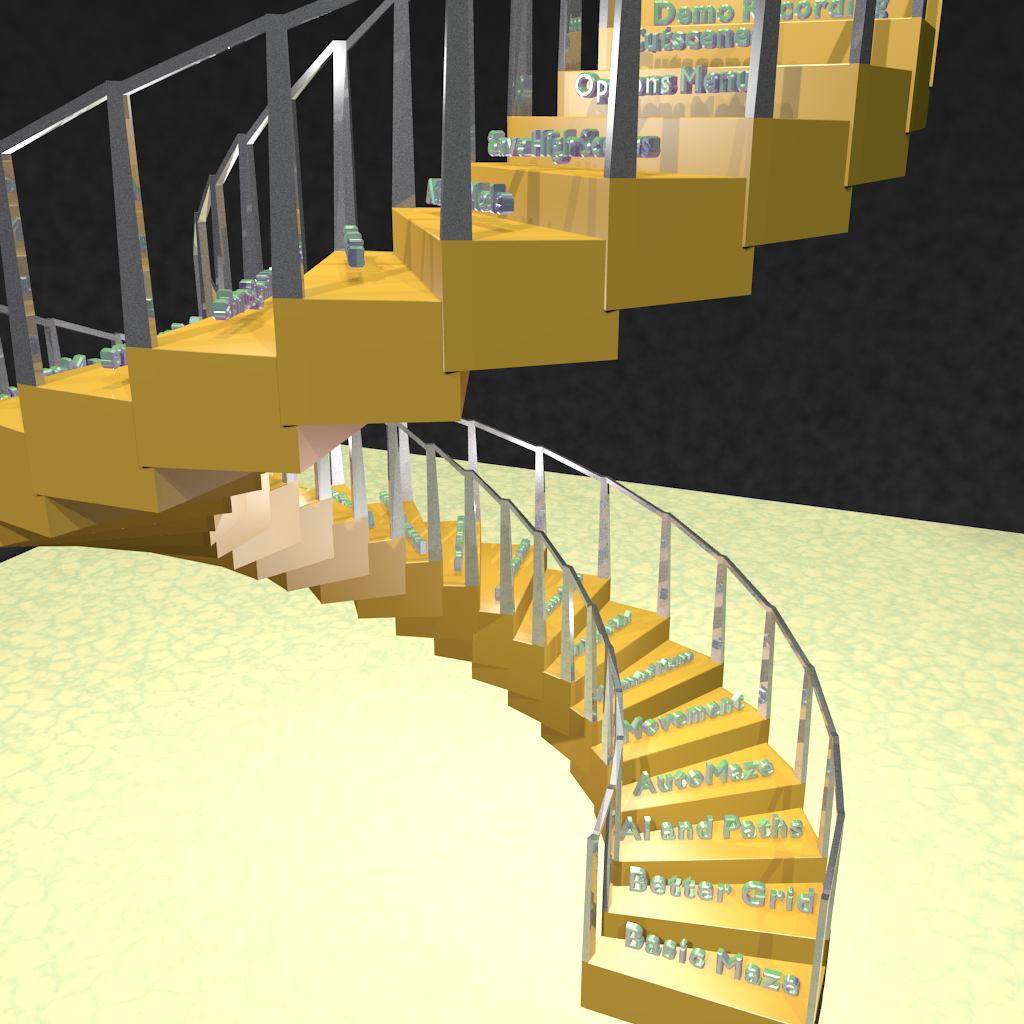
\includegraphics[width=3in]{SpiralBlocks.png}
  \caption{Spiral Design of Rat Race}
  \label{fig:spiral}
\end{figure}

When learning to build something complex, even creating a single piece of it might be beyond the ability of the beginner.  Thus, one has to build not the first building block, but a modest approximation to the first building block.  More modest approximations of building blocks are made, and a modest approximation to the whole game can then be made from them.  Next, we go back around to the beginning and improve those modest building blocks, one at a time.  Thus we have gone into a circle and the second time through, we are on a higher level.  Hence we have the “spiral” metaphor.  This metaphor applies both to building a game and learning anything complex.  See Figure \ref{fig:spiral}.

Think of building a house by first making a basic shelter from tree branches.  Later, time can be spent building a log cabin.  Later still, glass windows could be added.  Eventually logs will be supplemented with exterior siding and interior walls, and extras like plumbing and electricity can be retrofitted.  (Some buildings have been made following this pattern.  A historic building in my hometown started as a log cabin but was turned into a modern house.  In London, Westminster Abbey is a thousand-year-old stone building that has been retrofitted with plumbing and electricity.  If you can ever visit it, it's worth a tour.)

In the case of Rat Race, we start building a rough game with a really simple maze, using basic sprite assets that are really easy to create in minutes in GIMP.   It starts with a maze with a player in it that can’t move.  

Then, we add motion to the player.  We add dots that cannot be eaten and an enemy that cannot move.  However, to place the dots automatically, a simple AI framework is built.  This AI framework then is reused to make the enemy move aggressively toward the player.  In addition, the dots are made edible.  At this time, the game is a very rough prototype, but has much of the mechanics expected in the game.  The sprites are ugly, there is no score or leveling up or anything nice like that, but you can move the player, eat dots, and the enemy chases you.  This I call the “mechanic prototype” as it is useful for showing off the game mechanic to the boss or whoever you might be making the game for.  If your boss is an artist, he will not be happy with that, because it is ugly.

So the next cycle in the spiral is making all that look better, with sprites closer to what the game will ship with, better looking mazes, and so on.  Though the focus of this cycle is artistic in nature, much programming will still be done, because we would like levels to be generated automatically.

The next cycle is then to actually add game features to it: you can die, you can win the level.  That is the minimum to make it a game.  

Then we go back to the game mechanic.  Can we improve motion? We see what we can do about an awkward-looking glitch that happens every time either the player or the enemy goes around a bend.  We also add more enemies and different AI for different enemies.

Next, we improve the sprites even more, adding animations to them to make the game more fun.

Then we consider game state systems and build an Attract Mode, leveling up capability, multiple lives, and high score saving.  At this point, it’s a good game.

Finally, we improve level building and the multiple levels, consider extensive play testing, tweak the difficulty level, and other “last 1 percent” things that take at least 50\% of the total development time.  Only then is the game ready to ship.  So we discuss how to publish the game.

\section{Duties of the Reader/Student}

Plan to put quite a few hours into this course.  An hour each weekday is better than 10 hours every Friday, or you will lose your momentum.  Two hours each weekday is even better still.   However, five minutes every hour or continually while multitasking doesn't really do the job (The author even recalls a recent study that multitasking causes permanent changes in the brain that lowers a person's IQ....).  A continuous block of an hour a day most days of the week dedicated to focusing on just this project is close to optimal.  

What you get out of this course is a direct function of what you put in.  Try to make various concepts an integral part of you, rather than gaining a cursory understanding.  If your document reader or ebook reader allows you to do so (Acrobat Reader does: \url{https://get.adobe.com/reader/enterprise/}, and so does the Amazon Kindle device), highlight and add notes so you can quickly review sections of this document later.  At worst, you may have to kill some trees for the benefit of self-education (which is a funny way of saying, if nothing else works, take notes in a paper notebook).

Sections include theory as well as practice.  The theory is important for understanding.  Just as mankind did not understand how to put a man on the moon until people like Newton and Einstein wrote the theory, we cannot be effective game programmers without understanding the theory of state machines, AI, and so on.

In addition, references are given.  It is strongly encouraged to at least look at the free online references.  Some references requiring purchase, or at least a visit to a good university library or an interlibrary loan, are also helpful but are treated as optional.  These references give more depth to the topics covered.

\section{What This Book Covers}

\section{Software Needed}

The following software is recommended.  Unity 3D is the required one.  Other software is very useful but replacements can be found.

\begin{itemize} 
\item Unity 3D (Personal Edition is fine) Version 5.6 (slightly later versions will probably work) \url{https://unity3d.com/get-unity/download}
\item GIMP (GNU Image Manipulation Program) \url{https://www.gimp.org/downloads/}
\item Audacity (audio software) \url{http://www.audacityteam.org/download/}
\item Visual Studio Community Version 2015 \url{https://www.visualstudio.com/downloads/} (or MonoDevelop, included with Unity, if not on Windows).
\item Github Desktop App \url{https://desktop.github.com/}
\item SourceTree \url{https://www.sourcetreeapp.com/}
\item A web browser (for example, Firefox: \url{https://www.mozilla.org/en-US/firefox/products/})
\item A .pdf reader (to read this document).  Recommended is Acrobat Reader: \url{https://get.adobe.com/reader/enterprise/}
\end{itemize}

\begin{exercise}[Install Needed Software]
Using the urls provided, install as much of the above software on your system as you can.  If you get stuck, walkthroughs follow.  If you successfully install and are able to run any piece of software, you can skip the section for installing that piece of software.  If you can install and run it all (or have good alternatives), you can skip the rest of this chapter.
\end{exercise}

\chapter{Introduction to Unity}

\begin{figure}[h]
  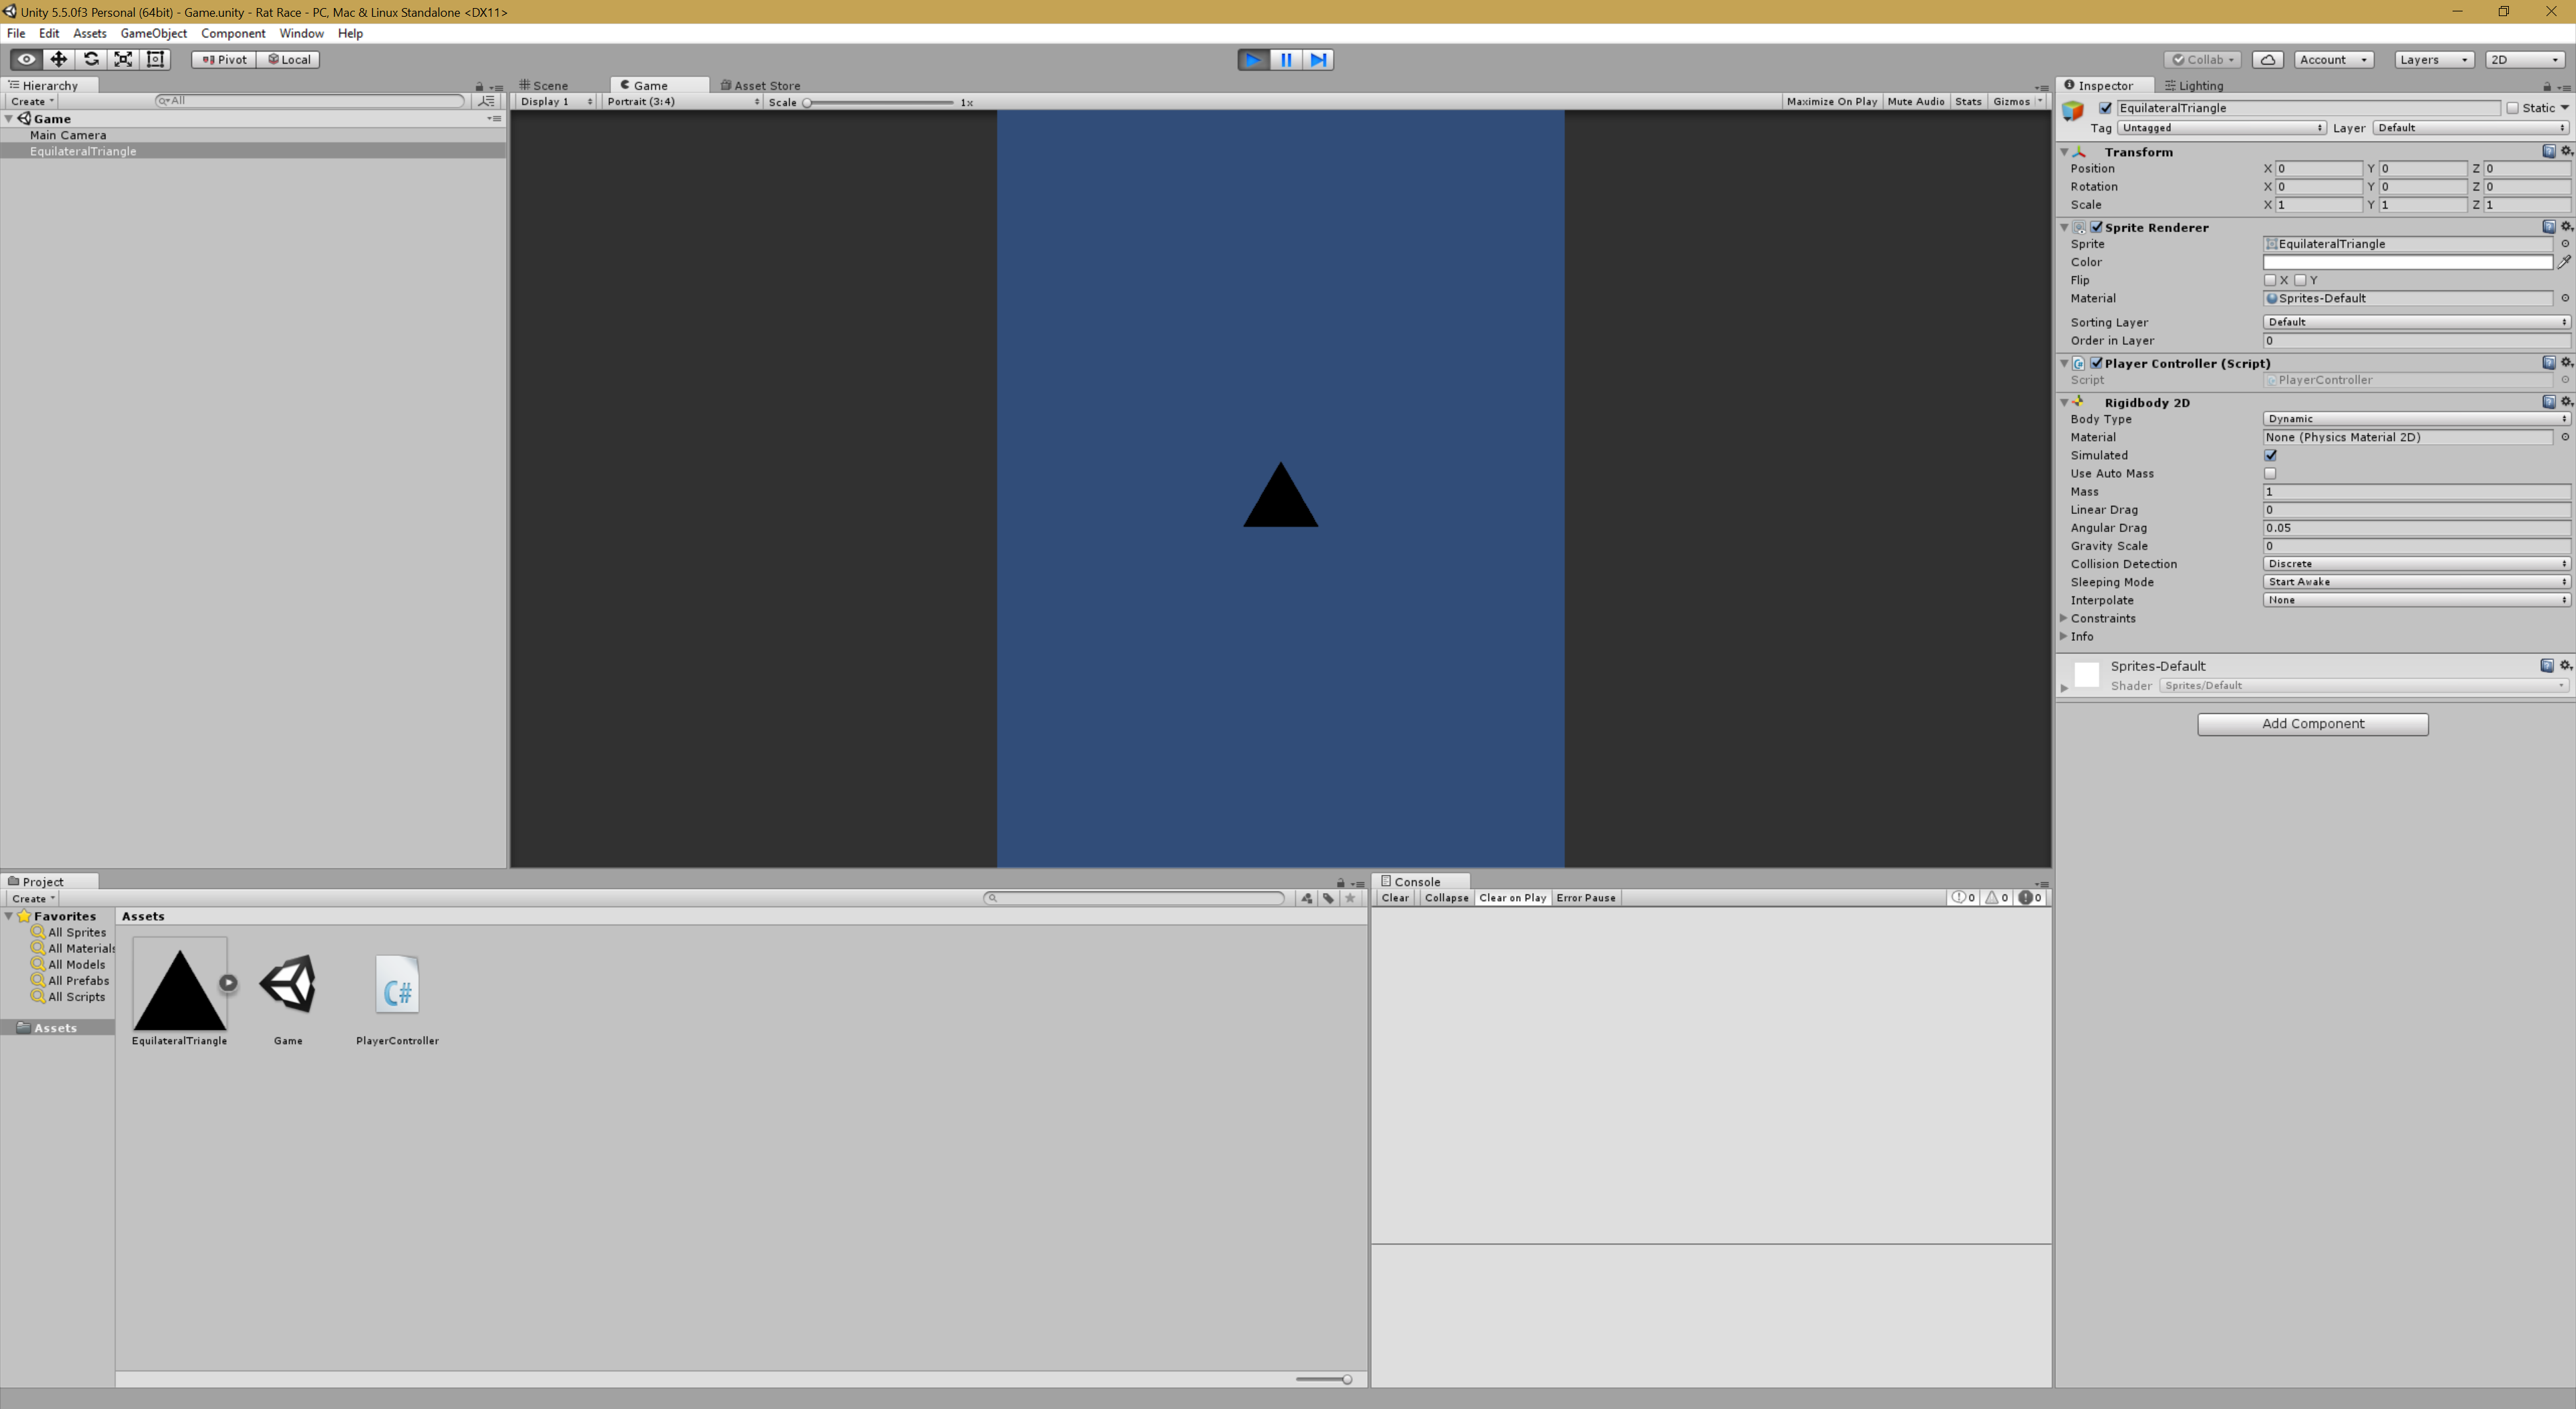
\includegraphics[width=3in]{prototype.png}
  \caption{Basic Prototype with Controllable Sprite}
  \label{fig:prototype}
\end{figure}


At the end of this section, we shall have the most basic behavior of an arcade game: a controllable sprite.  It’s not much.  Figure \ref{fig:prototype} shows the really basic “game”.  The purpose of the prototype is to have something, anything, that is visible progress in the development of the game.  This is what a programmer can show his boss while saying, "I did this today."


\section{Install Unity}
Before doing anything else, make sure you have time to install Unity.  There is a lot to install, so you might want to wait till just before bedtime and let it run overnight, for example.  The initial steps take about 15 minutes, then you let it run for perhaps hours.

Before installing Unity, just to be safe, close any open instance of Unity or Visual Studio or Monodevelop.  Running instances can interfere with the installation process.  (This has happened with the author, who installed Visual Studio Tools for Unity while Visual Studio was running.  No error messages and the installation was declared successful, just that Visual Studio crashed when opened from then on.  It took some Googling to find a fix.)  If you want to be really safe, close other programs too.  It is rare in modern days (with computers, the last few years is ``modern''), but still not unheard of, for software installers to crash a machine and cause you to lose data in open programs.

Go to the Unity download page: \url{https://unity3d.com/get-unity/download}.  Click the green "Choose your Unity + Download".  Look for the Personal edition (this is the free version) and click the green Download Now button.

Look at the green Download Installer button carefully.  If it says Version 5.6.something, you are good to go.  If not, you might still do ok if it is not far off, but if you really want to be safe (in particular, if you are a beginner), you would have to find the link near the bottom of the screen that says "Older versions of Unity" and click that, then find some version of 5.6.something in the list and download that. 

When you find Unity 5.6, click the appropriate download button to download the installer.  What happens next depends on your browser, but you could either just run it, or save it first, find where it was saved, and then run it.  You may have to give the computer or browser permission to install.

When this is done, the Unity Download Assistant window comes up.  Read and accept the license agreement.  (I know, nobody reads it.  A software company proved that once by offering a cash prize and it took 3000 sales before it was claimed: \url{http://techtalk.pcpitstop.com/2012/06/12/it-pays-to-read-license-agreements-7-years-later/}.  But, legal disclaimer, read it or suffer the fate of Dilbert: \url{http://dilbert.com/strip/1997-01-14}.) 

Check the ``Accept'' box after you understand all that legaleze (you do understand it all, right?).  Click "Next" or "Continue".  Select 64 bits if you can (a 64-bit system is strongly recommended) and click Next.  Any other screens that might have been added since this was written, read carefully and try to make the right decision and click Next, till you get to the Choose Components screen.  Now some decisions need to be made.

The defaults are probably OK for most people.  You definitely want to install Unity, and install the documentation and standard assets.  The example project is completely optional.  If you are on Windows, you want to install Visual Studio along with Visual Studio Tools for Unity.  Otherwise, MonoDevelop.  Then what remains is optional depending on what you want and where you want to deploy games.   If you have the disk space and don't mind waiting a while to install, it's ok to just check everything.  If you leave something out, it is possible to add it later from within Unity.

Click Next.  Downloading to a temporary location is recommended.  Most people can keep the default install folder, but if you want multiple copies of Unity, you have to make sure they are in different folders.


\begin{figure}[h]
  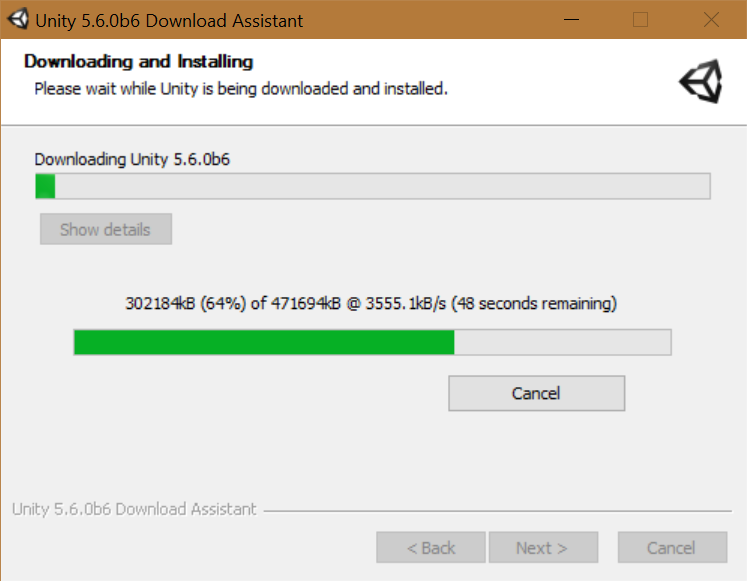
\includegraphics[width=3in]{InstallUnity.png}
  \caption{Unity Installer Has a Lot of Work Left to Do}
  \label{fig:install-unity}
\end{figure}

Click Next and wait (Figure \ref{fig:install-unity} shows 48 seconds remaining from one component.  The upper bar shows there are many, many more components left to install.) It takes time.  If you checked a lot of optional components to install, it takes a lot of time.  

Follow any remaining instructions.  Note that if you want to have multiple versions of Unity at the same time, you will have to change the directory it installs to, because by default, it writes over whatever version you have already.  Otherwise, you can leave the default.  For Mac, you may have to move another version somewhere else first, then install.  Now is a good time to walk away for maybe even a few hours.  But note that you may have to clear a popup or two during the install (e.g. Visual Studio already up to date--the author got this popup installing the beta version, but not the final version, so it ``should'' not be an issue if not using a beta version).  To be safe, visit the computer from time to time to OK/Continue any popups.

When done, test that it works by running Unity 3D.  You may be asked to give it access to private networks.  Do this, but not to public networks, whose safety cannot be guaranteed.  Feel free to watch any videos or browse any new user introduction documentation.  If you have not done so already, Unity will require you to register.  There are no serious side effects to doing this, and they send hardly any e-mails.

\section{Install Visual Studio If Needed}

\begin{figure}[h]
  
\includegraphics[width=3in]{vsweb.png}
  \caption{Install VS2015 Community Edition if Needed}
  \label{fig:vsw}
\end{figure}
  
This step should not be necessary because the Unity installer should do it for you (if on Windows; Mac uses MonoDevelop instead and this section does not apply).  However, if the Unity installer did not do this already, and you do not already have Microsoft Visual Studio 2015, you need to install it (by the time you read this, if you are using a version of Unity later than 5.6, it may be that it uses Visual Studio 2017 instead; if so, install that instead).  The free community edition is fine.  Go to \url{https://www.visualstudio.com/downloads/} (Figure \ref{fig:vsw}) to get to the download page.  If it does not say Microsoft Visual Studio 2015 (and you are using Unity 5.6 which uses version 2015) you may have to do some Googling to find the older version, if a link isn't already on the page somewhere.

Otherwise, under the Visual Studio Community section, click the blue Free Download button.  What happens next depends on your browser, but you could either just run it, or save it first, find where it was saved, and then run it.  You may have to give the computer or browser permission to install.

When this is done, the installer window comes up.  Just follow the instructions.  The default settings should be ok, except be sure that \csharp is included with the installation.

\section{Optionally Install GIMP}
Go to the page at \url{https://www.gimp.org/downloads/} and click the appropriate installer button.  What happens next depends on your browser, but you could either just run it, or save it first, find where it was saved, and then run it.  You may have to give the computer or browser permission to install.  Follow the instructions, accepting the license agreement.

\section{Game Objects and Prototype Assets}
Let us create some reusable prototype sprite assets.  To do this, we use GIMP, though if you are comfortable with another graphics editor, go ahead and use that.

We shall create several prototype sprite images that will be useful for not just Rat Race, but other games you may wish to build later.  These sprites are placeholders until we create something better.  They are just for getting started and moving forward quickly.


\begin{figure}[h]
  \includegraphics[width=6in]{shapes.png}
  \caption{We Shall Create These Shapes}
  \label{fig:shapes}
\end{figure}

The prototype shapes we shall make are:

\begin{enumerate}
\item A circle
\item A square
\item A diamond
\item A rectangle twice as high as wide
\item A rectangle with ``golden'' aspect ratio
\item An equilateral triangle
\item An isosceles triangle that fits in a square
\item A right triangle that fits in a square
\item A regular hexagon
\item A regular octagon
\item A hexagon that fits in a square
\item An octagon that fits in a square
\end{enumerate}

These shapes will be 256 units wide, a reasonable size, particularly given that some graphics cards can optimize shapes whose dimensions are a power of two.  They will be white on a transparent background.  They are white so that Unity can easily recolor them to any color (Unity uses a ``multiplicative'' model to recolor sprites).  We show all the shapes (in blue rather than white) that we shall create in Figure \ref{fig:shapes}.


\subsection{Running GIMP}
First, start up GIMP (or your favorite graphics editor, but the instructions here assume GIMP).  It may take time the first time it is run because fonts and scripts needed to be loaded and cached.

The author prefers the GIMP layout to be a little different from the default.  This is a user preference, but if you do not already have a preference, consider these.

First, let us select ``Single Window Mode''.  When GIMP opens up the first time, there are three separate windows.  Worse, if you have multiple monitors, they are spread around among the monitors.  That is the first thing to fix.  Find the main window (with ``GNU Image Manipulation Program'' in its titlebar, and the ``Gimp'' creature with eyes and ears in dark gray over a light-gray background, not the Layers-Gradients or the Toolbox windows) and under the Windows menu option, select the ``Single Window Mode''.  This will simplify GIMP usage greatly.  The Toolbox and Layers windows are now merged with the main window.

The remaining preferences are set through the Edit menu, Preferences selection.  A popup window labeled Preferences now lets you change almost anything about GIMP.  If you mess up too badly, you can always hit the RESET button, which will also reset to multiple window mode, but you know how to fix that now.

Here are the author's recommendations for preferences:

\begin{enumerate}
\item Under Environment, change Minimum number of undo levels to 100
\item Under Help System, check if there is a warning that ``the user manual is not installed locally''.  If you see this, you have two options: either return to the GIMP webpage and download and install the user manual and set the User manual option to Use a locally installed copy, or make sure the User manual option is set to Use the online version.

\item Under Tool Options, check the ``Save tool options on exit'' box.  You can reset a tool option at anytime if you do not like what it was saved to.  Also, check the ``Set layer or path as active'' box, which ensures if you click on something with the move tool, it becomes the active layer to be moved.

\item Under Toolbox, check all three boxes at the top: Show foreground and backgroudn color, Show active brush, pattern, and gradient, and Show active image.

\item Under Default New Image, change Image Size to 256x256.  Change ``Fill with'' option to Transparency.

\item Under Default Grid, the black default color is too often invsible on images used in games.  Click the black box following ``Foregroudn color'' to bring up a color chooser dialog.  Under the HTML notation, type: 1ecbb5 to make it a medium blue-green.  Change grid spacing from 10x10 to 32x32.
\end{enumerate}

After setting all the preferences, click OK to finish.

\subsection{Draw a Circle in GIMP}


\subsection{Draw a Square in GIMP}

\subsection{Draw a Diamond in GIMP}

\subsection{Rectangle 1:2}


\subsection{Rectangle Golden}

\subsection{Equilateral Triangle}

\subsection{Isosceles Triangle}

\subsection{Right Triangle}


\subsection{Regular Hexagon}


\subsection{Regular Octagon}

\subsection{Hexagon 1:1 and Octagon 1:1}

\section{Initial Unity Scene}\label{sec:unity}
Open Unity.  You may be asked to sign in.  If you have a registered Unity account, use the e-mail address and password for that.  If not, click ``Create New'' and follow the instructions to create a new account with Unity.

\begin{figure}[h]
  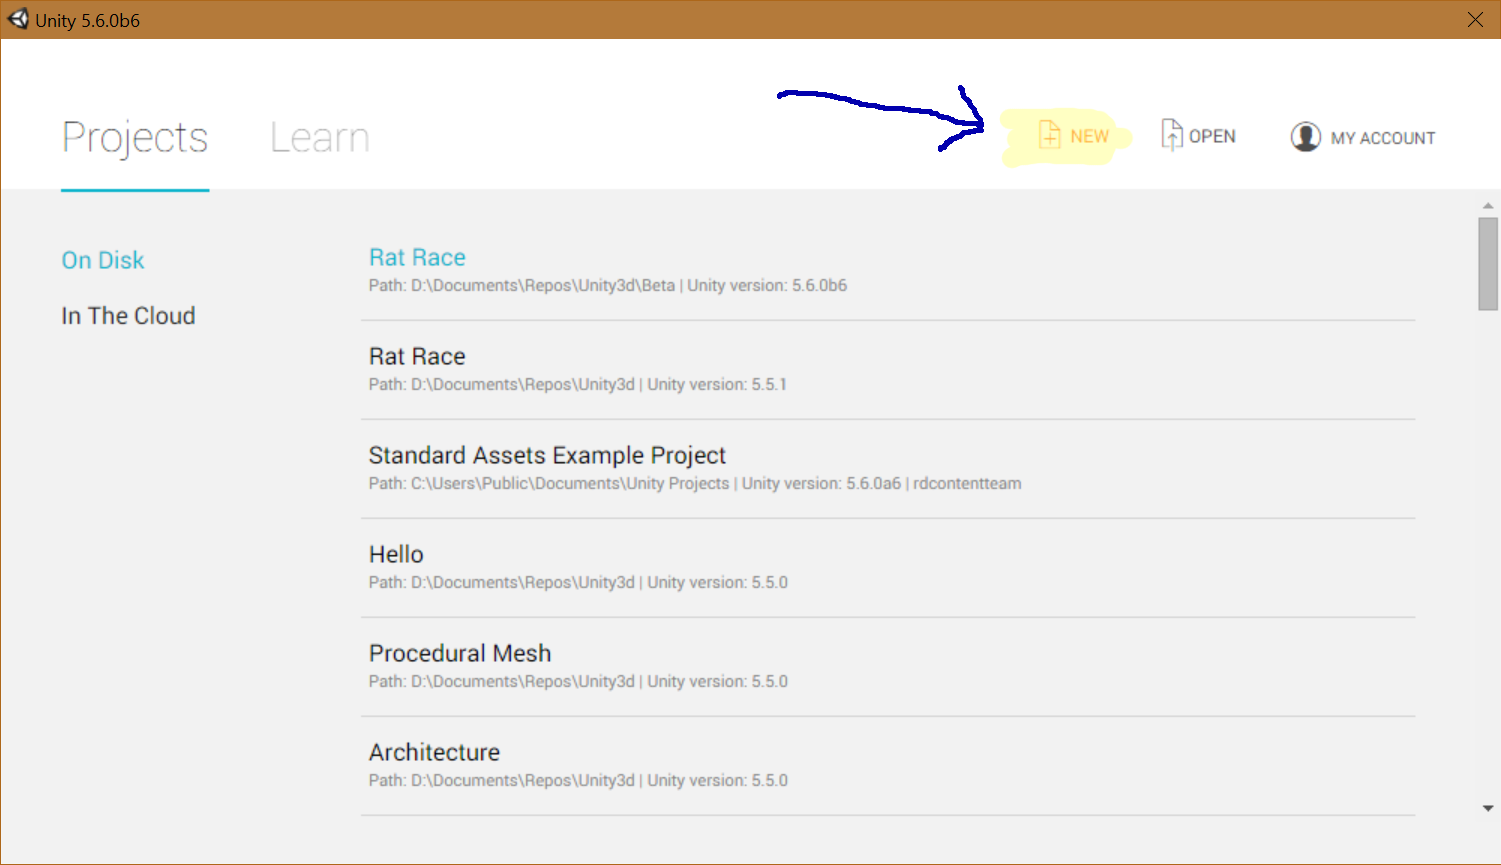
\includegraphics[width=4in]{NewButton.png}
  \caption{Create a New Project in Unity}
  \label{fig:new-button}
\end{figure}

After all this is done and you are signed in, the Projects window will appear.  Click the New button, with the icon that looks like a dog-eared sheet of paper with a plus sign on it (Figure \ref{fig:new-button}).

Enter the name Rat Race for the project name.  Choose a location that is convenient and that you can find again easily.  You are probably a member of just one organization unless you set up more, so either accept the default organization, or if you set up more, choose the one you want.

Change the 3D to 2D, since this is a 2D game.  We will not add any asset packages yet.  This can be done later anyway.  Go ahead and leave Unity Analytics enabled--that seems harmless at worst.  Finally, click the blue ``Create Project'' button and wait a minute for the project to be created and the Integrated Development Environment (IDE), which is also called the Unity Editor, opens. The screen will look something like Figure \ref{fig:unity}.

\begin{figure}[h]
  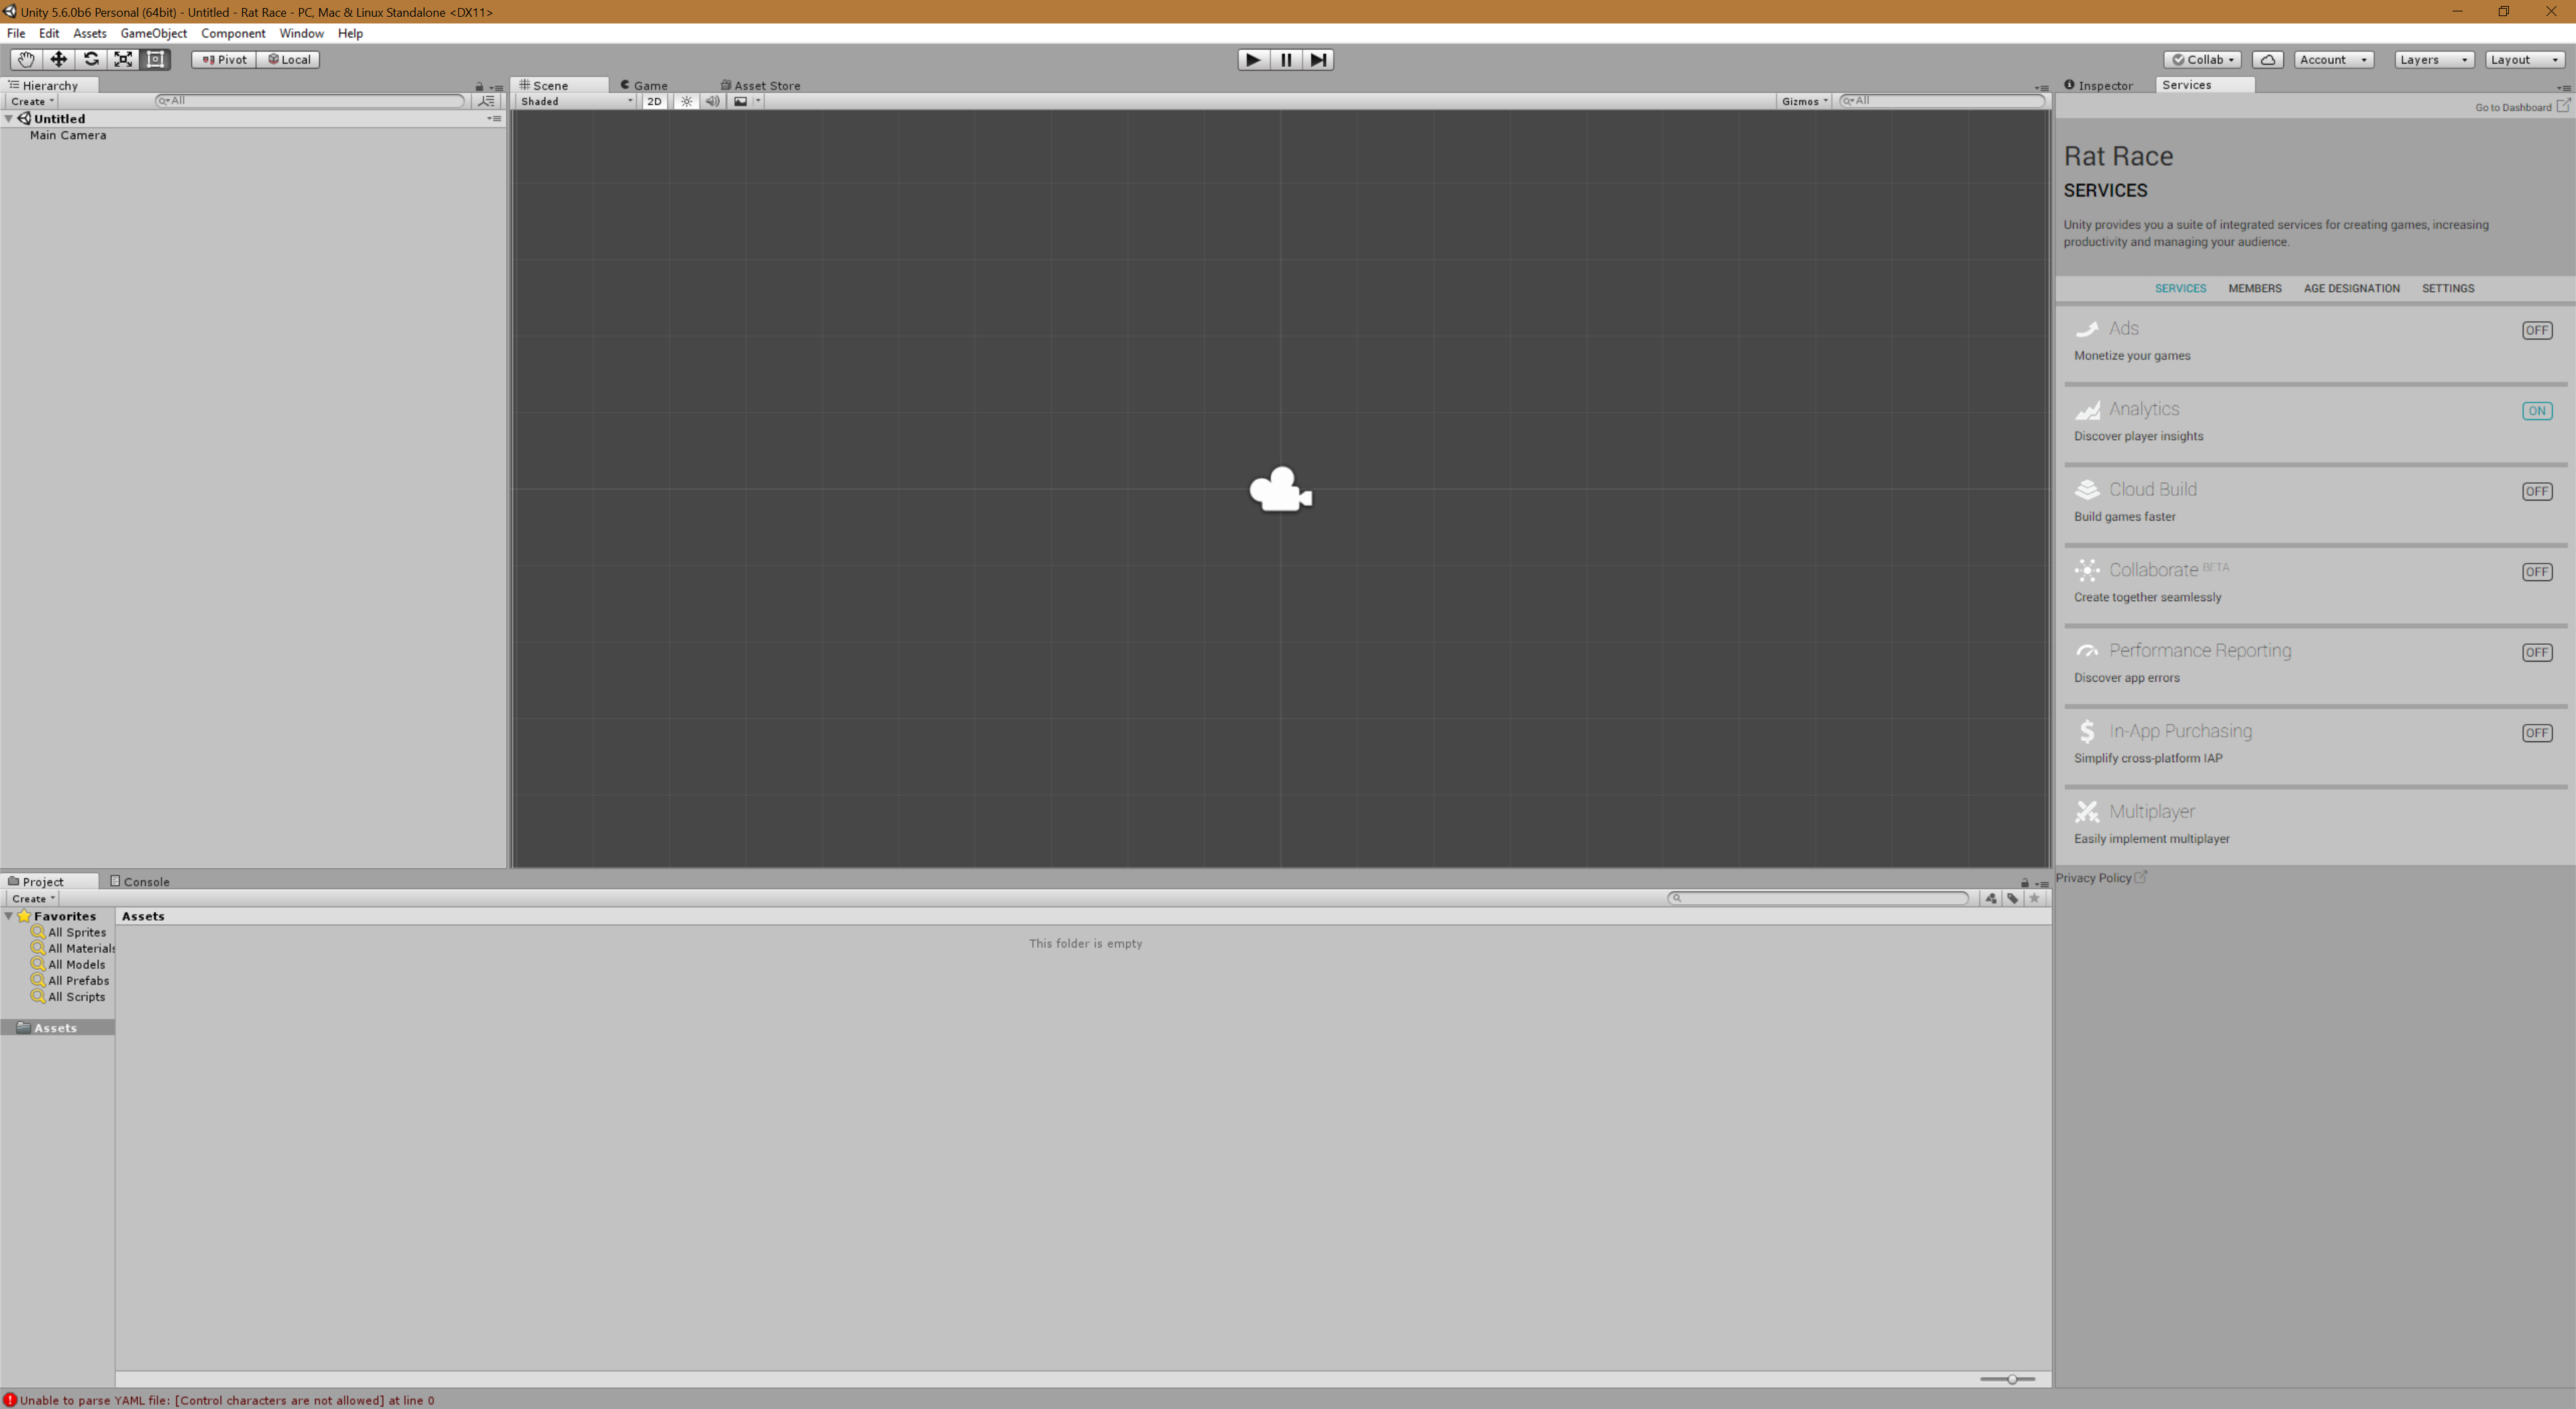
\includegraphics[width=6in]{Unity.png}
  \caption{Screenshot of Initial Unity Scene.}
  \label{fig:unity}
\end{figure}

\subsection{Brief Tour of Unity}

Let us look at the default layout.  We describe everything briefly, but some of these things we shall cover again as they are needed, and with more detail. At the top is the menu bar with File, Edit, Assets, and so on, menus.  Just below that is the header bar.  On the left are a hand icon, four arrows icon, two curved arrows icon, four diagonal arrows icon, and a box icon.  These are the manipulators.  For example, the box icon is the 2D rectangle manipulator, while the four arrows (up, down, right, and left) is the position manipulator for moving objects around.  The hand is the ``pan'' manipulator for panning the screen around.  The curved arrows are for rotating objects, and the diagonal arrows are for scaling (resizing) objects.

Just to the right you see Pivot and Local buttons (by default).  The first button says which part of an object is ``focused'' for rotation, and so on.  If you click it, it changes to Center.  Click it again to set it back to Pivot.  Every object has a pivot point, defined when the object was created, but it might be different from the center point, which is defined by its geometry.  The Local button tells which space coordinate axes are in: local (centered on the object) or global (centered at the world origin point which may or may not be near the object).

Toward the middle is a right-pointing triangle (Play), a double vertical bar (Pause), and a right-pointing triangle against a vertical bar (Step).  The Play button runs the game.  You can press it now, but the ``game'' won't do much yet.  It may take a few seconds the first time to set things up, then an empty blue game screen will appear, and the game button will turn blue to show that the game is playing.  Press the Play button again to stop.  The Pause button will pause, or resume, a running game without stopping it.  If the game is paused, the Step button steps forward one frame.  This is sometimes useful for debugging a game.

All the way right are more buttons: Collab, a cloud icon, Account, Layers, and Layout.  We do not use these much.

Then, the remainder of the IDE window is divided into panels.  The top left panel is the Hierarchy panel, showing every object in our current scene.  The top middle panel is the one we use most, showing the scene.  Currently, it only has the camera in it.  Notice it has tabs at the top, so you can select a tab to switch from the Scene tab to either the Game tab or the Asset Store tab.

The top right panel currently shows the Services tab, but there is also an Inspector tab which we use more.  Go ahead and click the Inspector tab to bring that up.  Whenever an object is selected in the Hierarchy, the Inspector panel shows details for that object.

Then, at the bottom is the Project window, which will show all assets used in the game (currently, there are none).  There are tabs at the top here as well, and the other tab is the Console, which is useful when testing a game.  Log entries from a game are printed onto the console, and error messages show up there too.

It is possible to change the layout by dragging the lines between panels around to resize panels, or right-click the tab of a panel to close the tab or add a new tab.  If a tab is closed by accident, it can be reopened through the Window menu in the menu bar, and selecting the name of the panel to open.

It is also possible to drag tabs around, to move a panel to another location, or even undock it completely to make a new window.  If you do this accidentally and want to undo it, just click on the tab at the top of the window and drag it back into the main window.

\subsection{Set Up a New Scene}
With Unity open, switch from the Scene tab to the Game tab (with a PacMan icon) in the top middle window (in the default layout).  There are changeable options at the top of the game panel: Display 1, Free Aspect (by default), and scale, to the left, and Maximize on Play, Mute Audio, Stats, and Gizmos, and a downward-pointing triangle on the right.  We are interested in the ``free aspect''.  We wish to change this into a portrait mode standard definition game screen, which has ratio 3 to 4.  If you click, you see ``4:3'' is an option but (by default) ``3:4'' is not.  But you can click the plus sign on a gray disk to add a new option.  Make its label ``3:4''.  Change the type from Fixed Resolution to Aspect Ratio.  Finally, make the width 3 and the height 4.  

Now there is a new option in the aspect button called ``3:4''.  Select the ``3:4'' aspect, and the blue portion of the Game window will change shape to be tall but narrow.  Now, optionally, you can adjust the Hierarchy and Inspector to make them a little wider: you have the space to do that now.  Click the ``Scene'' tab (with the grid icon) to leave the Game panel and return to the Scene panel.

Let us now save the scene before continuing, just to make that a good habit.  Under File, select ``Save Scenes''.  The first time you save a scene, it will ask you for a name.  Call it ``Game'' for now (we shall create other scenes later).  Also for now, keep the default folder (the ``Assets'' folder top level).  We shall consider organization of assets later.

\subsection{Orthographic Camera and 3D Coordinates}
In the Hierarchy panel to the left, select the ``Main Camera'' that was put into the scene by default.  At least two things will be noticeable when you do this: there is a Camera Preview box in the scene panel (currently showing nothing but a field of blue), and the Inspector panel is now populated with the camera's properties.  It is this Inspector we are interested in now.

The objects in the Hierarchy (except the ``Game'' scene object with a little Unity Cube icon next to it) are ``GameObjects'' (Unity uses just one word for it: GameObject). When you selected the only game object in the scene the Inspector panel showed the ``Components'' of the object: the Transform component, the Camera component (every Camera game object has a Camera component, a strange reuse of terminology), a GUI Layer, a Flare Layer, and an Audio Listener.  We shall be mainly interested in the Transform and Camera components for now.

Each component then has several ``Properties'', some of which have values that the user can change.  For example, the Transform component has Position, Rotation, and Scale properties, each of which has an X, a Y, and a Z field.  The values are floating point numbers shown in the boxes.  These can be edited.

By default, the camera is at position $x=0$, $y=0$, and $z=-10$, or more succinctly, $(0,0,-10)$.  Note the world origin (mentioned before) is at $(0,0,0)$.Thus, the camera is ten units away from the world origin, in the negative $z$ direction.  What does this mean in terms of the geometry of the scene?

The first thing to note is that there are three coordinates even though we selected a 2D game when creating the project.  This is because Unity is a 3D program.  2D work is essentially fit into a 3D framework.

Now, Unity uses the same left handed coordinate standard found on most graphics cards.  The $x$ direction is from left to right (in particular, (-2,0,0) is two units to the left of the origin, and (3,0,0) is three units to the right of the origin).  The $y$ direction is from bottom to top (so (0,5,0) is five units above the origin, for example),  The $z$ coordinate is front to back, that is from the position of the user sitting in front of the monitor toward a point behind the monitor.  One can imagine the monitor screen itself being at $z=0$.  The camera, as we saw already, is at $z=-10$, so it can be imagined sitting 10 units in front of the monitor, perhaps where the user is sitting.  (How big is a unit? In the game in 3D mode, a unit is often taken as a meter, but in 2D mode it is all ``shrunk'' (the word is actually ``projected'') onto a flat monitor, so if you try to map units on the $z$ axis out of the screen into the real world, it really depends on the zoom level of the camera lens.)

The rotation values show the amount of rotation, in degrees, about the $x$ axis, the $y$ axis, and the $z$ axis.  This is (0,0,0) for the camera, so the camera is unrotated, in its default position pointing toward the back of the monitor.

The scale values show how much the camera has been scaled along each axis.  These are all 1, so the camera is unscaled (scale being a multiplicative factor, not an additive quantity, has 1 for its identity, not 0).  Camera scale does not actually mean much, because one never sees the camera in the game, so it is usually left unchanged from the default.

Is this really where we want the camera? It turns out, no.  We discuss this next.

\subsection{Game Coordinates}

We shall build the game on a grid, 48 squares wide by 64 squares tall (which gives the 3:4 ratio).  We discuss why later.  We would like the (0,0) square (these will be game coordinates) to be at the bottom left of the camera's field of view, and therefore the (47,63) square will be at the top right.  We actually want (0,0,$z$), in world-space coordinates to be the \emph{center} of the lower-left square, and (47,63,$z$) to be the \emph{center} of the upper-right square.  Thus, the center of the camera should be aimed at the arithmetic mean (average): $(\frac{47}{2}, \frac{63}{2}, z)$.  We shall keep $z$ at $-10$ so the camera is 10 units in front of the grid.

Therefore, we need to set the Transform component's Position property to $x=23.5$, $y=31.5$, and $z=-10$.  So, with the Main Camera game object selected in the Hierarchy panel, adjust the $x$, $y$, and $z$ fields of the Position property of the Transform component to have these values.  Leave the other values unchanged.  The camera may disappear off the Scene view when you do this.  You can get it back by finding it by panning (right-click and drag) the view, or just double-click the Main Camera game object in the Hierarchy to center the view on the Main Camera.  Optionally, also use the scroll wheel on the mouse to zoom in and out.

We are not done.  The camera is positioned right, but we need to set the field of view.  In a real camera, this would involve choosing a lens and adjusting the focus and zoom.  In Unity, we adjust the properties of the Camera component.

First, the Projection property should already be set to ``orthographic''.  If not, make the change.  The choices are Perspective or Orthographic.  The former is for 3D games (though some older top-down games used an orthographic camera) and shows the view in proper perspective with far objects appearing at a smaller scale than near objects.  Orthographic cameras don't actually exist in real life (but can be approximated with a very expensive lens with a very, very short focal length) but with an orthographic camera, objects are not scaled by distance.  A one meter cube fills the same amount of screen space whether it is 1 meter away or 1000 meters away.  This is what we want with a 2D game.

The other property we need to look at is the Orthographic Size, just shown as ``Size'' in the Inspector panel.  This is equal to the half-height of the camera in game coordinates (called Game Units).  Since our grid is 48x64, the height of the grid is 64, and the half-height is 32.  So, we set the Size property of the Camera component to 32.  Now, the camera field of view (shown as a white rectangle in the Scene view; you may have to zoom out to see it) will exactly cover the grid.

The remaining properties can be left at their default values.

Now, if we were to place a sprite at $(0,0)$ (and it doesn't matter what the $z$ is as long as it is greater than -10 or it will not be visible because it would be behind the camera), it will be placed on the lower-left grid square.  If you place multiple objects there, those with lower $z$ values will be in front of those with higher $z$ values and will either partly or completely obscure those behind it.

\subsection{Importing Assets}
Open up a Windows Explorer or Macintosh Finder window and navigate to the folder where the prototype shapes were stored: Circle.png, Diamond.png, Hex\_1\_1.png, HexRegular.png, OctRegular.png, Rectangle2h.png, RectangleGolden.png, Square.png, TriangleEqui.png, TriangleIso.png, and TriangleRight.png.  Also make sure the Unity window is visible with the Project panel open to the Assets top level.  Select these 11 files and drag them into the Assets area.  All 11 should then automatically be imported into Unity and get icons that look like thumbnails of the shapes.

There is still some work to do.  Select each of the 11 new assets, one at a time, in the Project panel.  As each is selected, import settings for the asset will appear in the Inspector.  Find the Pixels Per Unit property under the Sprite Mode.  It defaults to 100.  Change it to 256.  Do the same for all of the 11 new sprite assets.  A shortcut is to select all of the 11 sprites (Ctrl-click or on a Mac, CMD-click), but be sure nothing else is selected.  Then when you change Pixels Per Unit in the Inspector, all 11 are changed.  Click the Apply button at the bottom right of the properties shown in the Inspector to save the change.  The click a few of the shapes individually to confirm the change went through and that the Apply button is now grayed out.

This means, 256 pixels of the sprite will correspond to one game unit.  So, all the sprites will be exactly one grid square wide.  We can still scale the sprites individually as they are placed in the game, but we want a reasonable default to start with.

\subsection{Creating a Prototype Maze}

Now, let us start building the prototype game.  We shall use the isosceles triangle for the player and the hex\_1\_1 for the enemy.  Go ahead and drag these into the Hierarchy panel.  Then select each one in the Hierarchy panel and adjust their Transform component properties: the $x$, $y$, and $z$ scale of each should be 3 (we want the player and enemy to be three grid squares wide).  Set the position of the triangle to (2,2,0), and of the hexagon to (45,61,0), thus putting them at opposite corners.  

Next, right-click on the TriangleIso sprite in the Hierarchy and select Rename.  Change its name to Player.  Then, right-click on the Hex\_1\_1 spirte in the Hierarchy and select Rename.  Change its name to Enemy.

Now for each of the two sprites in the Hierarchy, look at their Sprite Renderer components.  For the triangle, click on the colored bar next to the Color property, and use the color chooser to change it to yellow (Hex FFFF00FF).  Close the color chooser when done.  Also, follow the same steps to change the hexagon's color to red (Hex FF0000FF).  Note that in Unity the hex values for a color have 8 digits, not 6 like GIMP.  GIMP's hex value has two digits each for the hexadecimal value of red, green, and blue.  Unity has these three as well, as well as ``alpha'' which is the opacity: 00 means invisible, FF means completely opaque, and values in between are different levels of transparency.  Thus, we set the triangle to all red and green with no blue and full alpha, which is yellow (red and green light mix to make yellow light), and the hexagon was full red, full alpha, but no green and blue.  With years of practice, one learns to visualize what hex values correspond to what colors.  The color chooser lets you choose visually as well as by hex values, to make it easier.

Next, put a square into the Hierarchy.  Change its coordinates so that they are integers.  Now, if you look at the manipulator buttons at the top left of the screen and select the four arrows pointing up, down, left, and right, the ``position'' manipulator, you can then move the sprite around by dragging the arrows (to drag horizontally or vertically), or the little square joining the arrows (to drag in anywhere on the plane).  Hold down the Ctrl (Mac: CMD) key while dragging it will keep it on integer values, which is what we want.  Put the block anywhere you want that way, but make sure the coordinates are integers.  

With the block still selected, hit Ctrl-D (CMD-D on Mac) to duplicate it.  Ctrl-drag to position it.  Do this multiple times and make part of a maze.  Don't bother making a complete maze, this is just for illustration.  We shall eventually use a Procedural Content Generation (PCG) maze, that is, one generated automatically.  File menu, then Save Scenes to save your work.


\begin{figure}[h]
  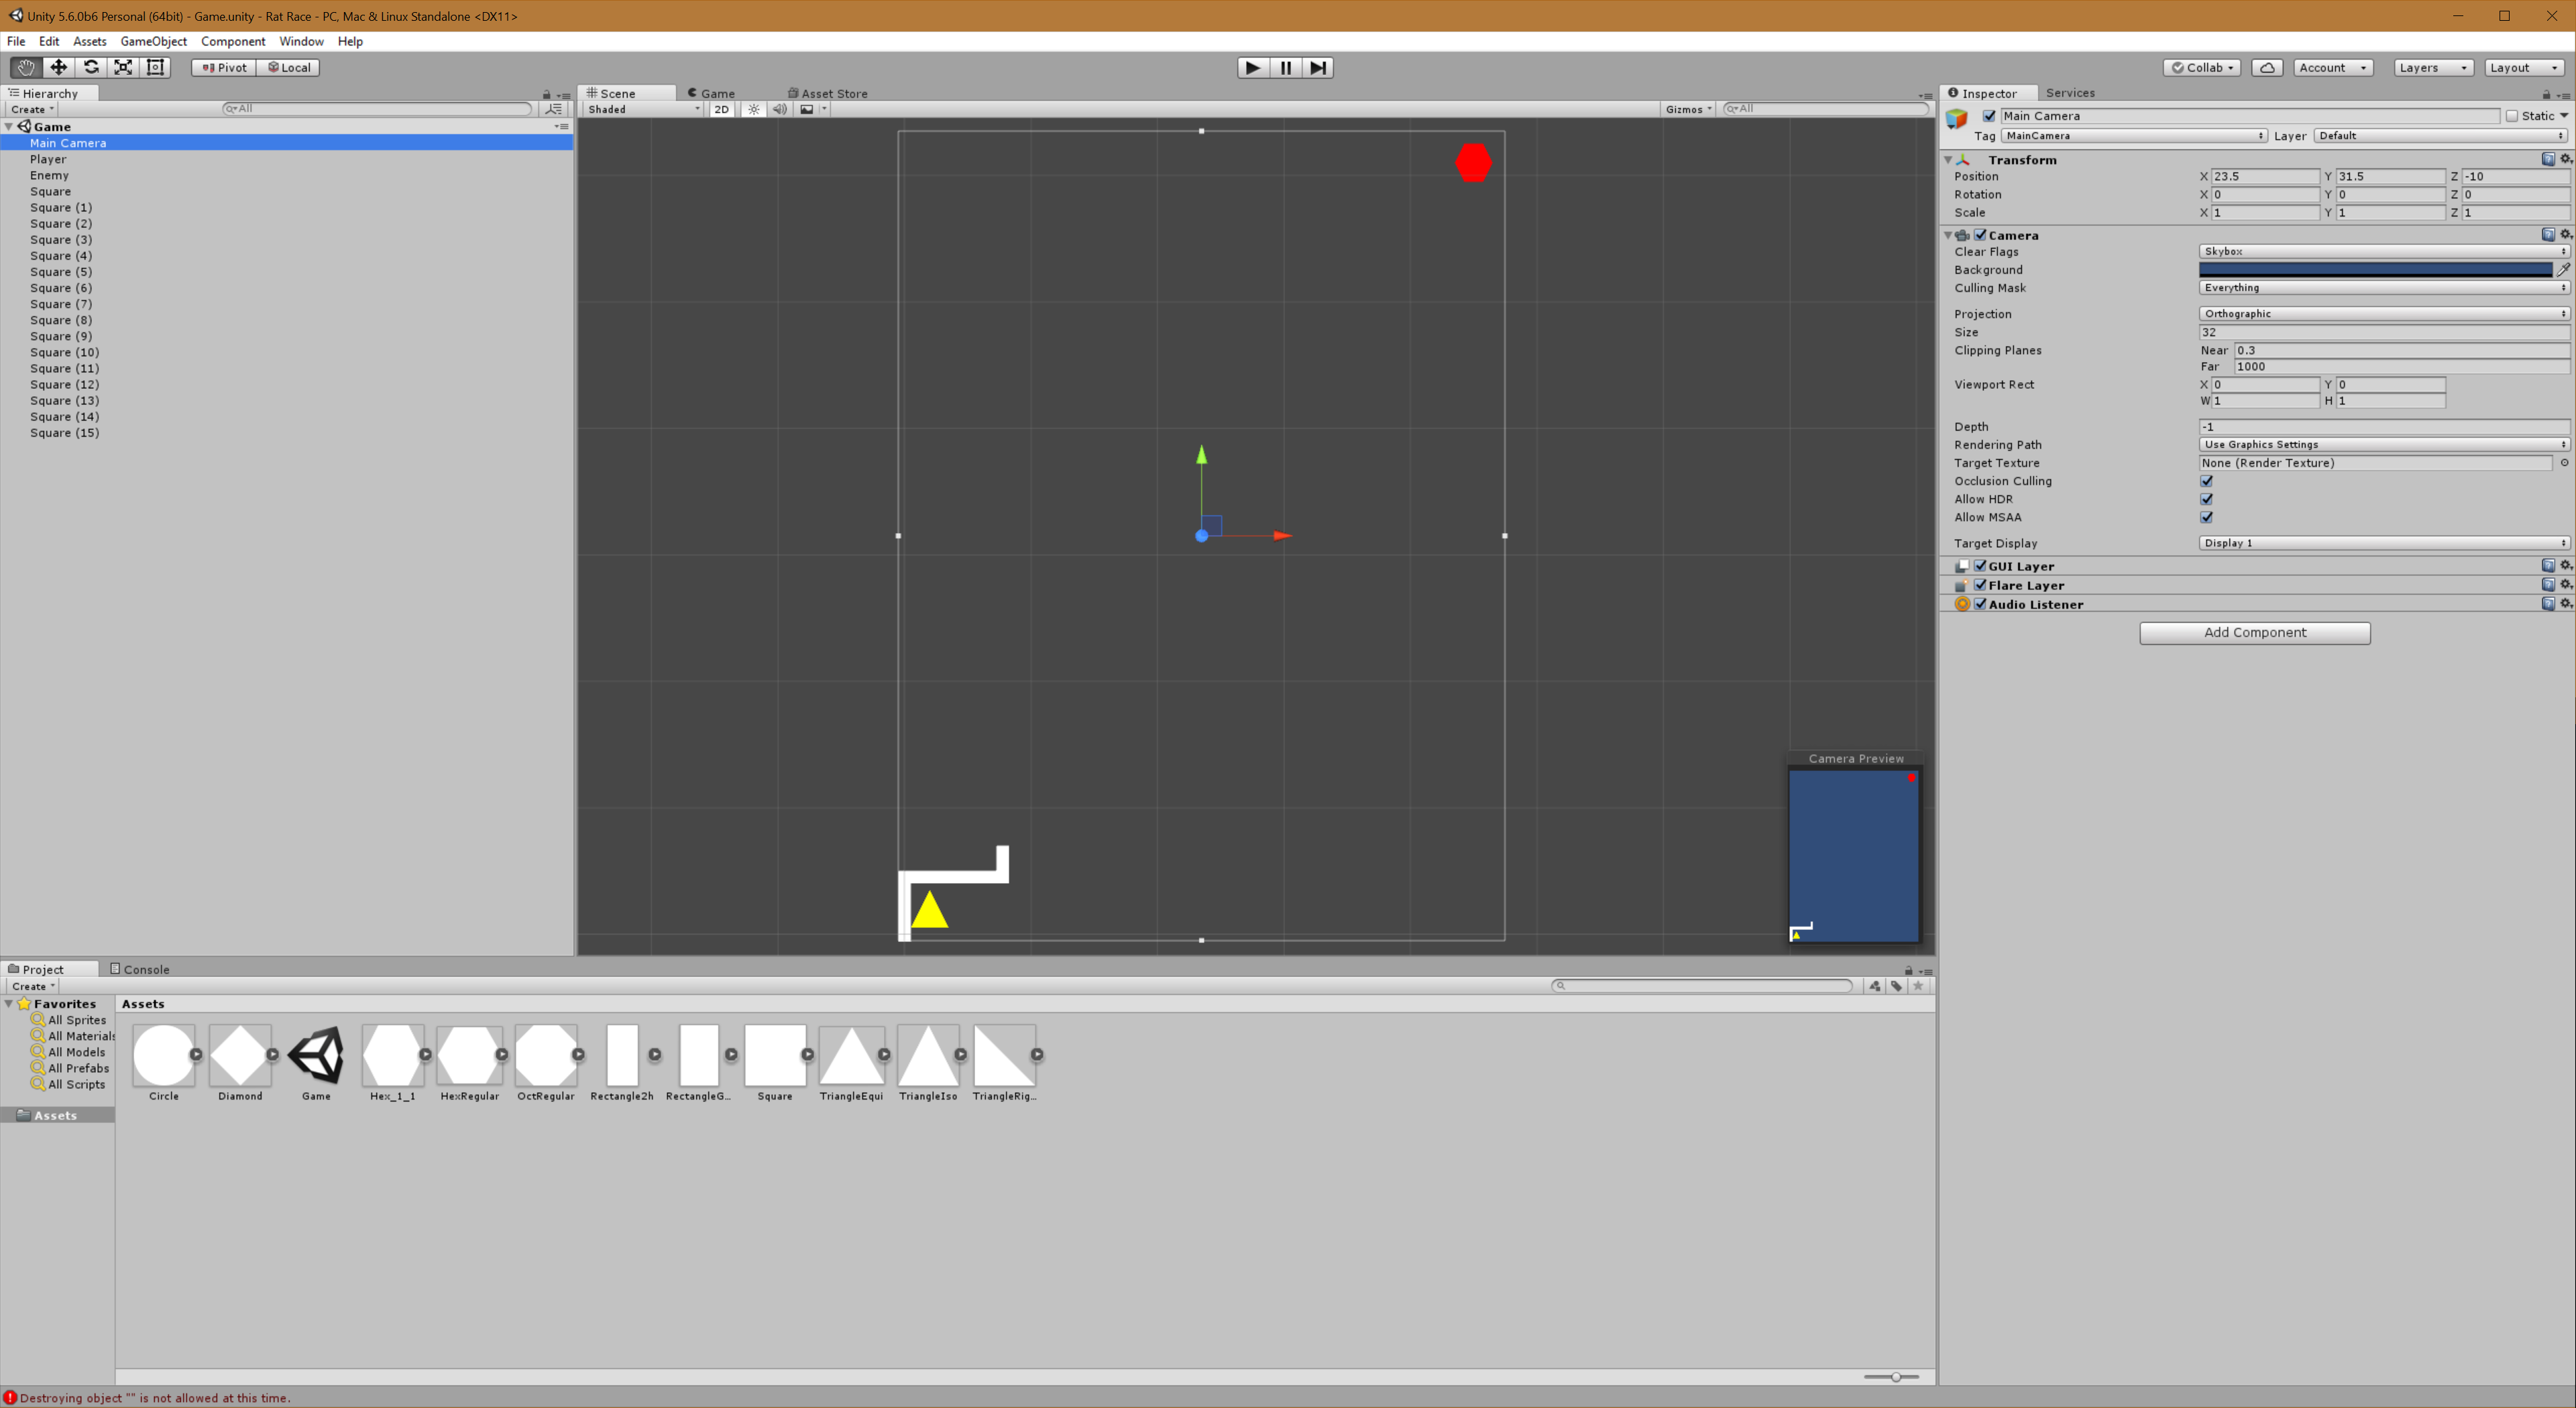
\includegraphics[width=6in]{ProtoMaze.png}
  \caption{Screenshot of Prototype Maze}
  \label{fig:protomaze}
\end{figure}

We now know how to put objects into a scene to make games.  See Figure \ref{fig:protomaze} for an idea of what the screen should look like now (though the walls might be in different places).  If you play the game now, you will see that prototype maze, but it will not do anything.  We address this in a later section.

\chapter{C Sharp Programming I}


\section{Unity \csharp}


\begin{exercise}[Hello World]
Open a new, empty project in Unity...
\end{exercise}


\section{Analysis of our \csharp Program}

\begin{exercise}
Go through the “Hello” script again and make sure you know what each item is.  
\end{exercise}

\begin{exercise}
Modify the Hello script...
\end{exercise}

\section{Compiling and Linking}

\section{A First Refactor}

\begin{review}
Check your knowledge by answering these questions, in your head, with regard to the script above.  If you are unsure of any answer, review the above notes to find the answer.
\begin{enumerate}
\item Is Debug an identifier, a keyword, or a string?
\item Is Debug the name of a class, a method, a namespace, or an object?
\item Is public an identifier, a keyword, or a string?
\item Is "Tick" an identifier, a keyword, or a string?
\item Is the occurrence of "Tick" in the program above an argument, a method, or a namespace?
\item Is Log an identifier, a keyword, or a string?
\item Is Log the name of a class, a method, a namespace, or an object?
\item Is UnityEngine an identifier, a keyword, or a string?
\item Is UnityEngine the name of a class, a method, a namespace, or an object?
\item Is the code beginning with "void Start" a method call or a method definition?
\item Is the code beginning with "LogTick()" a method call or a method definition?
\end{enumerate}
\end{review}

%\section{Syntax and Parsing}
%\cite{ALSU06}
\chapter{Non-Game Prototype}

\section{Adding Motion to the Game}

\begin{task}
Modify the GetInput method definition so that...
\end{task}

\subsection{Using the Input Manager Window}

\subsection{Adding Physics Components}

\subsection{Making the Sprite Move}

\subsection{Speeding Up the Motion}

\subsection{Adjusting the Speed}


\subsection{Collide with the Walls}

\section{Design Decisions for the Grid}

\begin{figure}[h]
  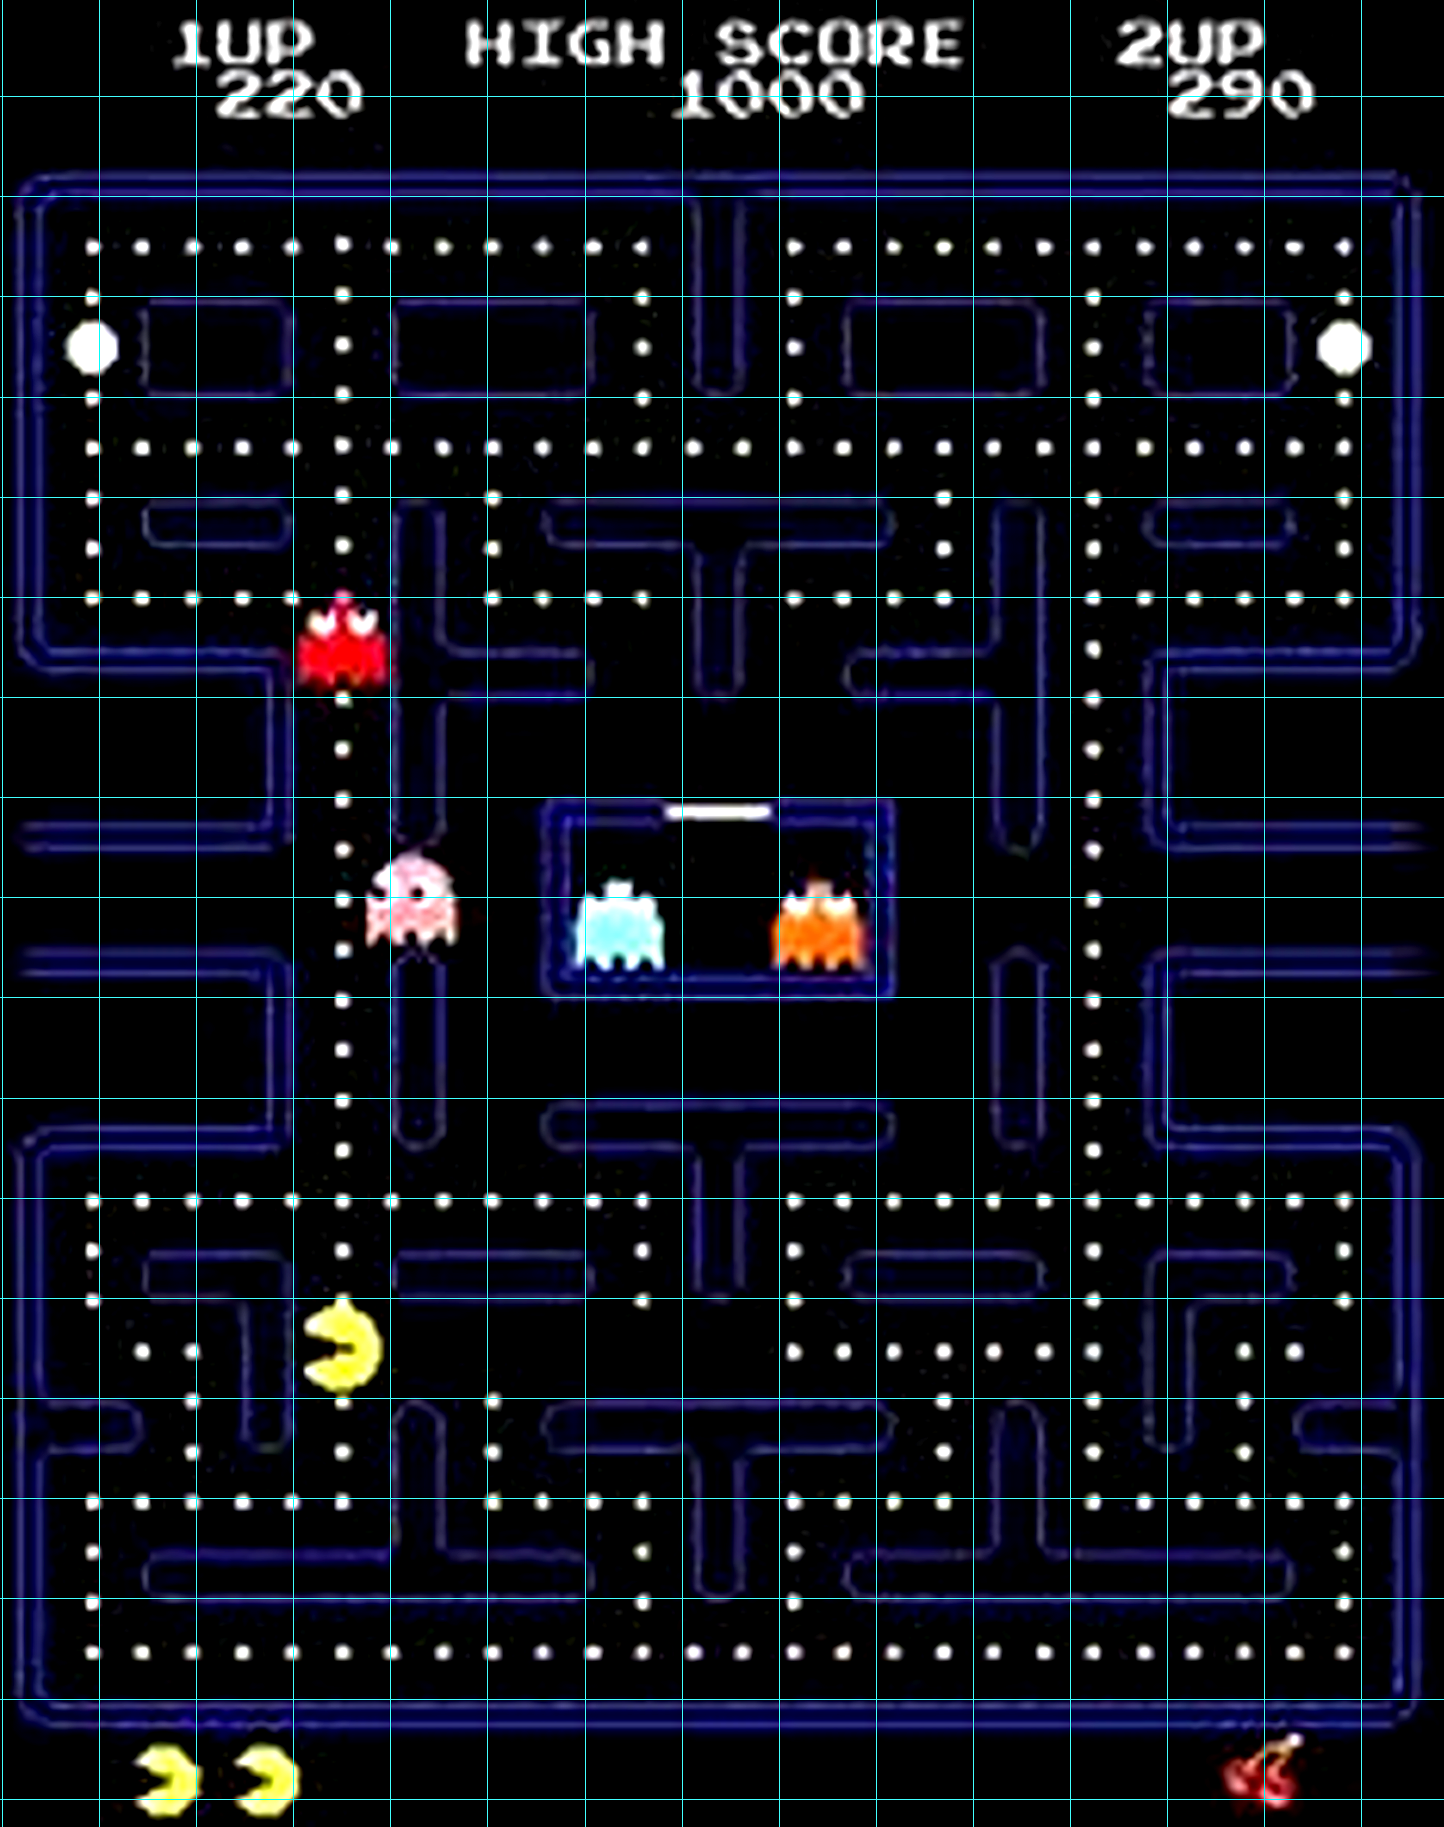
\includegraphics[width=3in]{PacManGrid.png}
  \caption{PacMan was not built on a grid}
  \label{fig:pacmangrid}
\end{figure}

\section{Building the Grid}

\section{Our Prototype So Far}


\chapter{Source Control}

\subsection{Setting up Github}



\subsection{Installing SourceTree}


\subsection{Putting Rat Race under Source Control}

\subsection{Publishing Rat Race to Github}

\chapter{\csharp Programming II}

\section{Types}

\subsection{Numeric Types, Casts, and Rounding}

\subsection{Boolean Types}

\subsection{Structs}

\section{Collections}
\subsection{Arrays}


\subsection{Multi-Dimensional Arrays}

\subsection{Sets}

\subsection{Queues}

\section{Scope and Visibility}

\section{Control}
\subsection{If Statements}
\subsection{For Loops}

\section{Random Number Generation}

\section{Annotations}

\section{Unity Constructs}
\subsection{Vectors}
\subsection{Unity Annotations}


\chapter{Automatic Maze Generation}

Let us now work on automatically building a maze.

We wish to have a game with a (seemingly) limitless variety of mazes.  One way to accomplish this is to generate the mazes automatically.  There are various maze generation algorithms out there, but most are for the kinds of mazes that have dead ends and only one path from start to finish.  We wish to have a different kind of maze, one that is closer in spirit to the "maze" of streets in, say, lower Manhattan.  But without the dead ends.

So, let us consider what kind of maze we want to generate.

\begin{figure}[h]
  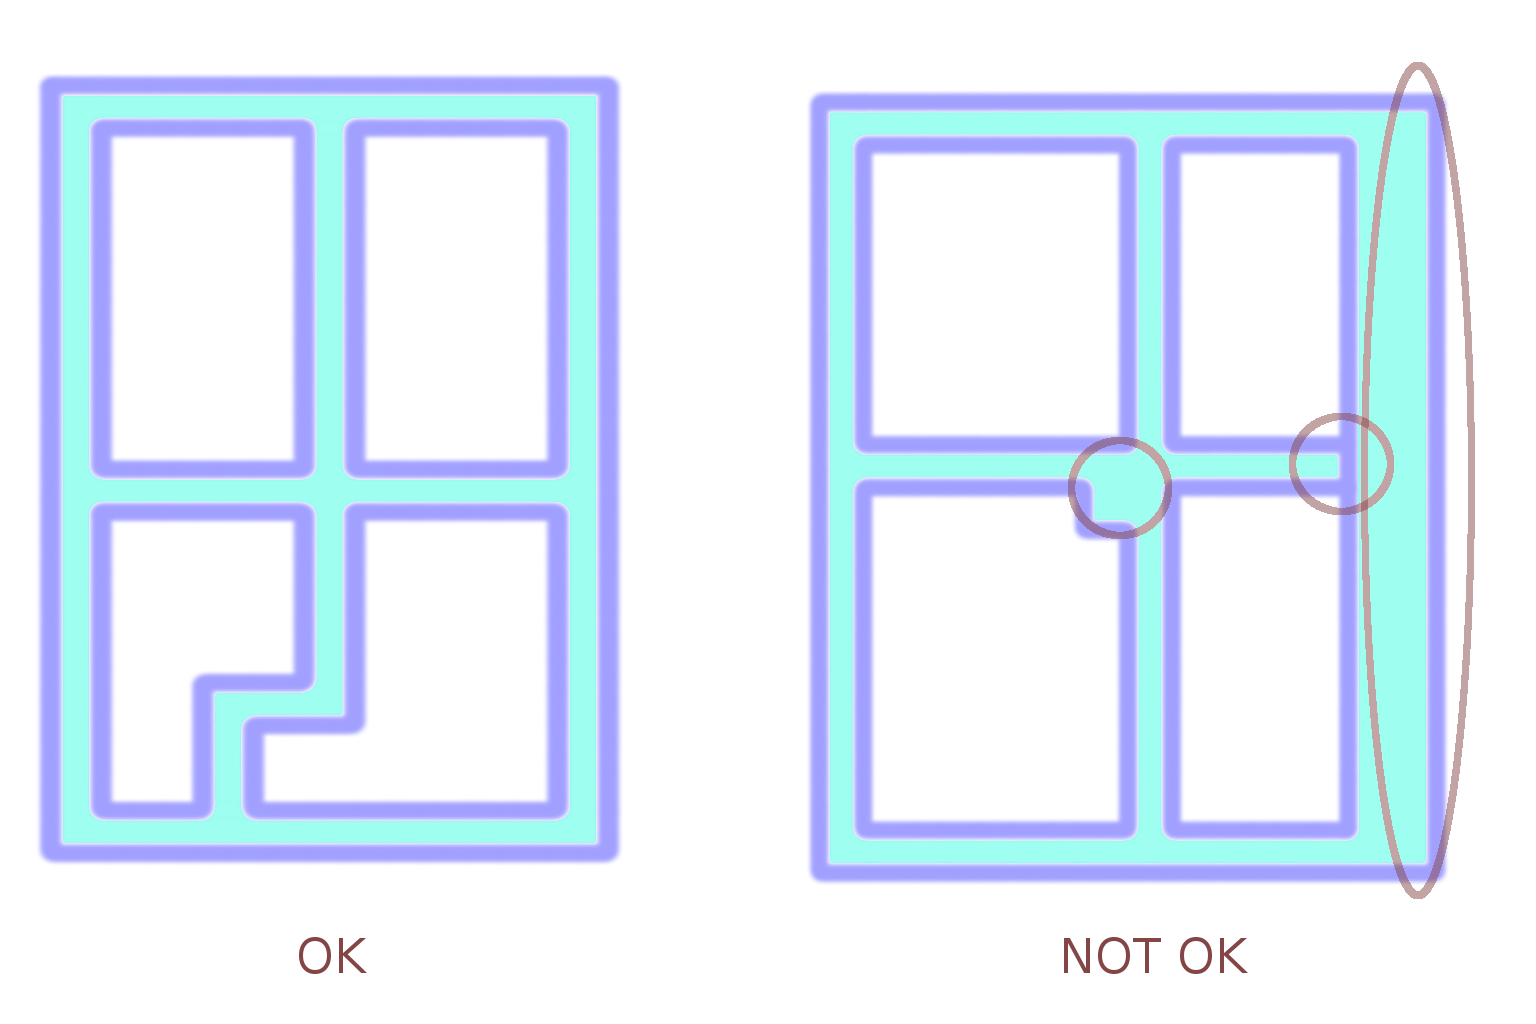
\includegraphics[width=3in]{Linear.png}
  \caption{The maze should be linear, with no "wide paths"}
  \label{fig:linear}
\end{figure}
  
\begin{enumerate}
\item It must be connected (or at least, have a teleport between unconnected parts, but we shall consider this complication at another time).   That means, it is possible to move from any point on the maze to any other point.  

\item It should be "linear".  By that, it is meant, no double-wide paths, even for a short distance.  See Figure \ref{fig:linear} for what is meant by this.  The left image is ok, but the right image has two wide paths and one dead end.  (Light blue represents the path here.)

\item It should have no dead ends (Figure \ref{fig:linear} has one dead end).

\item The paths should be as wide as the player sprite.  This is not the same as the grid square size, but is wider (3x wide to be exact).

\item The walls should be as thick as the grid square size (thicker is ok).

\item There will be some technical requirements.  These include, walls all around the play space (so the maze cannot be escaped), a place for the player to start and the enemies to start, and we will eventually want tunnels.
\end{enumerate}

Thus, it is necessary to come up with a procedure for randomly generating a maze satisfying the above conditions. 

\section{Playable Maze Design}
By looking at the original Level 1 PacMan maze, we notice the dots are arranged in 10 rows and 10 columns, with walls of various thicknesses in between.  This suggests a layout like this.

Let $m$ be the number of rows of dots and $n$ be the number of columns of dots desired.  Each path must be 3 squares wide and row and column paths have to be separated by one-square-wide walls, so this limits $m$ and $n$ so that $3m+m+1=4m+1\le64$ and $3n+n+1=4n+1\le48$, or $m\le{15}$ and $n\le{11}$.  If $m$ and $n$ are too small, it is not much of a game.  So, we make a design decision that $8\le{m}\le15$ and $8\le{n}\le11$.  

Once we choose $m$ and $n$, we can make a basic maze (that will be modified later) that is simply $m$ rows of dots and $n$ columns of dots.  We have some freedom in which to choose wall sizes between rows and columns.  If we make a design decision to make the border walls one square thick, then the paths between the borders take up $3m$ for row paths out of 62 grid squares and $3n$ for column paths out of 46 grid squares.  The $m-1$ walls between rows must be at least one grid square thick, and likewise for the $n-1$ walls between columns.  

Finally, note that in PacMan, the second row, second from last row, second column, and second from last column are all paths of dots.  We keep that design, which (for the start) gives us definites places for the player and an enemy.  Later we can modify this to make an enemy box and start the player somewhere deeper in the maze.

So, we pseudocode the algorithm to build the basic maze like this:

\begin{algorithmic}[1]
\REQUIRE{$8\le{m}\le15$ and $8\le{n}\le11$}
\ENSURE{A 64-row by 48-column grid has m row paths and n column paths such that no two row or column paths are adjacent and such that the first and last row and column are not paths, but the second and second from last row and column are paths}
\STATE{Start with a solid maze (all wall)}
\STATE{Carve a path in Row 1}\COMMENT{Rows are numbered from 0 to 63, and a row path will be carved from Column 1 to Column 46}

\STATE{Carve a path in Row 62}

\STATE{Carve a path in Column 1}\COMMENT{Columns are numbered from 0 to 47, and a column path will be carved from Row 1 to Row 62}

\STATE{Carve a path in Column 47}

\STATE{Create a row wall array $R$ of length $m-1$, initialized to all 1s}

\FOR{$i\leftarrow1$ \TO $62 - 4m$}
\STATE{Choose a random number $j$ from $0$ to $m-2$}
\STATE{$R[j]\leftarrow R[j]+1$}
\ENDFOR

\STATE{$r=2$}

\FOR{$i\leftarrow1$ \TO $m-2$}
\STATE{$r=r+R[i]$}
\STATE{Carve a path in Row $r$}
\ENDFOR

\STATE{Create a column wall array $C$ of length $n-1$, initialized to all 1s}

\FOR{$i\leftarrow1$ \TO $46 - 4n$}
\STATE{Choose a random number $j$ from $0$ to $n-2$}
\STATE{$C[j]\leftarrow C[j]+1$}
\ENDFOR

\STATE{$c=2$}

\FOR{$i\leftarrow1$ \TO $n-2$}
\STATE{$c=c+C[i]$}
\STATE{Carve a path in Column $c$}
\ENDFOR
\end{algorithmic}

\begin{exercise}
An actual PacMan maze (Google "PacMan" and look at the images) has a vertical line of symmetry.  Thus, the left and right halves are mirrored.  If you want a maze like this, modify the above algorithm to generate a symmetric maze.  Hint: $n$ will have to be an even number.
\end{exercise}

\begin{exercise}
An actual PacMan maze (Google "PacMan" and look at the images) has a "tunnel" row with no dots (except in vertical columns intersecting it).  It would be useful to require some row (other than Row 1 and Row 62) to be required to be a row of the maze, such as Row 31 so it can be made into a tunnel row.  Modify the algorithm to allow one row position to be specified while still drawing the rest of the maze correctly.  You may have to have separate cases for the tunnel row chosen to be an odd-numbered row versus an even-numbered row.  This is also optional: we shall add tunnels later.
\end{exercise}

\section{Starting the MazeBuilder Class}

Let us now write the MazeBuilder class that creates the basic maze so we can test it and see what it looks like.  

\begin{exercise}
The solution to this exercise follows, but try to do as much as possible before looking.  Create a new MonoBehaviour script called "MazeBuilder" attached to an empty game object of the same name.  Give it a new field:

\begin{verbatim}
private bool[,] grid;
\end{verbatim}
that will hold a 48x64 grid of booleans, where "true" indicates a wall and "false" indicates a path.  Recall the paths are three grid squares wide but walls can be any positive thickness.

Write a public Initialize method that initializes the array and fills the grid with nothing but wall, ready to start carving out paths.

Write a public CarveRow method that takes an integer $y$ value and carves out that row in the grid.  Do the same for a CarveColumn method. 

Finally, write a BasicMaze routine that takes parameters m and n and follows the algorithm just given to carve out m rows and n columns.
\end{exercise}

After completing the exercise, we shall have a script much like the following:

\begin{verbatim}
using System.Collections;
using System.Collections.Generic;
using UnityEngine;

public class MazeBuilder : MonoBehaviour {
    public int xSize = 48;
    public int ySize = 64;

    private bool[,] grid;

    // Use this for initialization
    void Start() {

    }

    // Update is called once per frame
    void Update() {

    }

    public void Initialize() {
        grid = new bool[xSize, ySize];
        for (int x = 0; x < xSize; x++) {
            for (int y = 0; y < ySize; y++) {
                grid[x, y] = true;
            }
        }
    }

    public void BasicMaze(int m, int n) {
        CarveRow(2);
        CarveRow(ySize - 3);
        CarveColumn(2);
        CarveColumn(xSize - 3);


        int[] RowWallWidth = new int[m - 1];
        for (int i = 0; i < m - 1; i++) {
            RowWallWidth[i] = 1;
        }
        for (int i = 0; i < ySize - 2 - 4 * m; i++) {
            int j = Random.Range(0, m - 1);
            RowWallWidth[j]++;
        }
        int r = 5;
        for (int i = 0; i < m - 2; i++) {
            r += RowWallWidth[i];
            CarveRow(r);
            r += 3;
        }

        int[] ColWallWidth = new int[n - 1];
        for (int i = 0; i < n - 1; i++) {
            ColWallWidth[i] = 1;
        }
        for (int i = 0; i < xSize - 2 - 4 * n; i++) {
            int j = Random.Range(0, n - 1);
            ColWallWidth[j]++;
        }
        int c = 5;
        for (int i = 0; i < n - 2; i++) {
            c += ColWallWidth[i];
            CarveColumn(c);
            c += 3;
        }
    }

    public void CarveRow(int y) {
        for (int x = 1; x <= xSize - 2; x++) {
            for (int j = y - 1; j <= y + 1; j++) {
                grid[x, j] = false;
            }
        }
    }

    public void CarveColumn(int x) {
        for (int y = 1; y <= ySize - 2; y++) {
            for (int j = x - 1; j <= x + 1; j++) {
                grid[j, y] = false;
            }
        }
    }
}
\end{verbatim}

\section{Testing the Result by Drawing It}

But how shall we test it? We need to actually draw the maze!  We use the "instantiate" function.  

\subsection{Prefabs}
Previously, we built game objects like the Player by putting an empty game object in the scene, then adding and modifying components one by one.  It is useful to save such a game object so it can be added (and perhaps then modified) again and again.  This saved game object is called a ``prefab'' asset.  When one creates a prefab, one can drag it into the scene.  Then, changing the prefab automatically changes the object in the scene (which is useful if you have lots of instances of the object and want to change all of them at once).  But if you change an instance in the scene, the change affects only that instance.

Another advantage to prefabs is we can instantiate them from code.  That is what we shall do with the ``wall'' prefab we create.

\begin{task}\label{task:prefab}
Select one of the wall components (one of the squares) in the Hierarchy.  Be sure it has a BoxCollider2D component on it.  Rename it to ``Wall''.  Now, make sure the Project (not the console) tab is shown below.  Drag the Wall object from the Hierarchy to the Project window.  A new asset called ``wall'' and showing the thumbnail of a square will appear in the Assets top-level folder.  This is a prefab.  Also, the Wall object in the Hierarchy will turn blue to indicate that it is linked to a prefab.

Now, select the Wall prefab in the Project panel.  Its properties will appear in the Inspector.  

Change its color to blue (Hex value 0000FFFF).  Note that the instance in the scene turns blue, but none of the other instances do.

Now, we do not want the walls in the scene anymore, because we are going to generate them automatically.  So, in the Hierarchy panel, select all the squares (including the Wall object linked to the prefab), and hit the delete key.  Be sure not to also delete the camera, the player, the enemy, or the maze builder objects.

Save the scene.
\end{task}

\subsection{Instantiation of Game Objects in Code}

Unity provides an ``Instantiate'' method (of the MonoBehaviour class) for instantiating a prefab into the scene.  The general procedure is as follows:
\begin{enumerate}
\item In a script, add a new public GameObject field for the prefab (with an appropriate name):
\begin{verbatim}
public GameObject somePrefab;
\end{verbatim}

\item In the code (for example, in the Start method), call the Instantiate method and set the return value to a GameObject variable:

\begin{verbatim}
GameObject someInstance = Instantiate(somePrefab, 
   positionVector3, rotationQuaternion, 
   optionalParent.transform);
\end{verbatim}
Here the positionVector3 is a Vector3 indicating where the prefab should be spawned.  The rotationQuaternion is its rotation, and is often just set to Quaternion.Identity (for no rotation). Optionally, a fourth field can be used to make the new game object a child of an existing game object (game objects can be in a hierarchy, as the name of the Hierarchy window suggests).  Use the .transform field of the desired parent.

\item Optionally, do something with the someInstance variable holding the instanced game object.  Destroy(someInstance) will destroy it, for example.

\item Now, compile the code.  If all goes well, there will be a new somePrefab field in the Inspector for the object that has this code as a component.  Drag the desired prefab into the somePrefab field value.  Then run the game to test.
\end{enumerate}

\subsection{Making the MazeBuilder Draw the Maze}

\begin{exercise}
Try writing code to draw the maze before looking at the solution below.
\end{exercise}

We add the following field at the top of the MazeBuilder class:
\begin{verbatim}
public GameObject wallPrefab;
\end{verbatim}

We can compile now, and the MazeBuilder object should have a ``wallPrefab'' field in the Inspector.  Drag the Wall prefab into that field.  It will now say ``Wall'' with a blue cube icon (the Prefab icon).

Now, we add a Draw method:
\begin{verbatim}
    public void Draw() {
        for (int x = 0; x < xSize; x++) {
            for (int y = 0; y < ySize; y++) {
                if (grid[x, y]) {
                    Instantiate(wallPrefab, new
                     Vector3(x, y,
                      wallPrefab.transform.position.z),
                       Quaternion.identity, transform);
                }

            }
        }
    }
\end{verbatim}

Finally, we call the Draw method  in the Start method.  We also add the maze creation method calls.  Change the Start method (currently empty) to match the following:

\begin{verbatim}
// Use this for initialization
    void Start() {
        Initialize();
        BasicMaze(10, 10);
        Draw();
    }
\end{verbatim}

We test with a 10x10 maze for now.  Run the game and test motion.  You will find a partially-built maze (the boring ``basic maze'') and that the motion only partly works.  See Figure \ref{fig:grid}.


\subsection{Fixing Glitches in Motion}

\subsection{The Code So Far}

\chapter[AI]{Artificial Intelligence: The \astar Algorithm}

\begin{challenge}
Write pseudocode for the general \astar algorithm.  Better still, write code for it either in \csharp or your favorite language, and test it on the example.  The specific case of ``\astar on a grid'' is given below, and can be used as a guide.
\end{challenge}

\section{\astar on a Grid}

\section{The Algorithm}

\section{Designing an Implementation of the \astar Search}


\section{Implementing \astar in Unity \csharp}

\subsection{Write the Program}


\subsection{The AStar Class}

\subsection{Testing the \astar class}

\chapter{Game Mechanics Prototype}

What do we still lack to make this a (lousy) game? We need enemies to avoid and goals to achieve.  Ultimately, the enemies will be cats and the goals will be in the form of edible dots.  For now, we use prototype sprites, using color to separate the roles.  We shall save for later niceties such as high scores, multiple lives, additional levels, and an “Attract Mode”.  But we can still make a simple score display and either end the game with level cleared (win) or end the game in a cat’s stomach (lose).

\subsection{Controlling the Enemy}


\subsection{Dots to Eat}

\chapter{Designing a Game}

Before improving this prototype, we shall ``go back to the beginning'', so to speak, and actually consider the design of this game.  When working on a large project, especially if there is more than one person, it is necessary to have a design in mind to focus the coding, testing, and asset creation.  The design is simpler than the actual project, so that it can be changed easily as needed.  In particular, it is easier to change the design than to change the working code.  Yet the design should be clear enough that different people working on different parts, or even the same person working on different parts at different times, can create things that fit together well.

Like with building the game and learning the techniques, a spiral approach is done, adding more detail to the design and improving the overall design in multiple iterations.  

The first iteration of the design has already been done, sort of, in Chapter 1, ``Let's Create a Game!''  Taking this chapter and ``tightening it up'' a bit and reorganizing it is a good first iteration of our design.  

The next section is our first attempt at a game design document.  The level of detail is not all that fine, but it should cover most of what the game entails.  Except for possibly the first paragraph, which is a marketing-type paragraph, it is intended mainly for those building the game, not for those playing the game.

The ``elevator pitch'' is what you say to someone on the elevator who asks you what kind of game you are making.  It is a very short description of what you are working on.  Every employee should have an elevator pitch: if you end up on an elevator with the CEO who asks you what you are doing, it looks bad to say, ``like, I don't know, nothing?''

The format of the Game Design Document is not set in stone.  This is but one way it can be done.  Googling for ``Game Design Document'' will get you plenty of examples to look at.  Some documents for big name studios producing big name games are very detailed.

\section{Game Design Document I}

\subsection{Marketing Statement}

Remember the Golden Age of the arcade, around the 1980s or so? It was a PacMan-eat-dot industry, where a game that didn't earn a quarter every three minutes got removed and replaced. The games were built to have lights and sounds to attract the player, and then to challenge the player enough that he's likely to lose the game...fast. Still, from time to time, a player would do really well and get on the high score list.

We shall build a game of this type. 

\subsection{Elevator Pitch}
The player controls a mouse who must eat all the cheese in the maze without being eaten by some very aggressive cats. 

\subsection{Technology}
We shall use the Unity game engine, whose software development editor and integrated development environment (IDE) runs on the PC and Macintosh, and can deploy games than run on the PC and Mac as well as the web and mobile devices and Linux.

We shall use Git for source control.

\subsection{Features}

\begin{itemize}
\item 2D classic arcade action
\item Written with Unity 5.6 and \csharp
\item Artificial Intelligence (AI) for the cats
\item Grid-based automated level building and Procedural Content Generation (PCG)
\item Score keeping with high-score saving
\item Multiple lives
\item Teleportation tunnels
\item Sound and music and animated sprite assets
\item A game state system managing the title and high score screens
\item Cutscenes
\item Published to multiple locations for multiple platforms
\item and more...
\end{itemize}

\subsection{Mechanics}
\begin{itemize}
\item Player is controled by a keyboard, joystick, game pad, or (for mobile devices) a touch screen, with inputs representing up, down, left, and right.  An input will change the direction of the player sprite (the mouse) to that direction if it is possible to go that direction.  Upon reaching an obstacle, the sprite will stop until a valid directional input is given.

\item The enemy sprites (cats) will be controlled by AI and will try to catch the mouse.  If the mouse is caught, a life is lost.  Initially, the mouse has three lives but new lives are sometimes given as a bonus.  When all lives are lost, the game is over.

\item The mouse must eat all the dots (cheese) in the maze, at which time a newer, harder maze is given (levelling up).  

\item Special ``growth hormone'' cheese gives the mouse the ability to chase and eat the cats for a short period of time.

\item Tunnels allow the mouse (or cats) to teleport, thus confusing the AI of the cats.  

\item Scoring is based on cheese eaten, cats eaten, bonus pickups eaten, and levels achieved.  Top scores are saved.
\end{itemize}

\subsection{Attract Mode}
\begin{itemize}
\item When the game is not in progress, it cycles through a title screen, a high score screen, a details screen, and a demo screen.  The demo is a video clip of sample gameplay.

\item An options button, leading to an options screen, is available.  User-selectable options include music volume, sound effects volume, and perhaps other options.

\item Attract mode ends when a ``Play'' button is pressed, and resumes on end of game (perhaps with a high score screen interlude).
\end{itemize}
\subsection{Assets}
Assets include an animated mouse, animated cats, cheese (dots), walls pieces, maze designs, sound effect clips, and level music. 

\subsection{Ideas for Future Development}
\begin{itemize}
\item Adrenaline: start with high reserve, low usage.  If mouse is near cat, can use it to go faster, but reserves are depleted and mouse slows down.  Need a ``run key'' (or maybe double-tap direction key) to signal ``use the adrenaline now''

\item Eating cats makes mouse full when growth hormone runs out and he walks slower for a time

\item Cat seeing mouse directly ahead gets excited and runs faster, but tires out quickly and time needed to have speed burst again

\item Mouse eating growth hormone cheese makes cats faster in running away in fear for a short interval of time

\item Special animation frames: mouse sniffs nearby cat and looks afraid, cat sniffs nearby mouse and looks hungry, etc.

\item Special pickups for special powers?

\item Dangerous ``pickups'' like a marching mousetrap?

\end{itemize} 

\section{Rapid Prototyping}

\section{Game Architecture}

\section{Game Engine Architecture}
\cite{Gre14}

\section{Level of Detail in a Design}
\cite{GHJV95}


\chapter{Creating Game Art I: The Mouse}

\section{Creating the Mouse}

\subsection{Google for Mouse Images}

\subsection{How does a Mouse Walk or Run?}

\subsection{Draw a Concept Mouse}

\subsection{Creating a Sprite Sheet}

\section{Animating the Mouse Bones}

\chapter{Creating Game Art II: The Cat}

\section{Creating the Cat}

\subsection{Google for Cat Images}

\subsection{Draw a Concept Cat}

\subsection{Creating a Sprite Sheet}

\section{Cheese for Dots}


\chapter[Improving Maze Walls I]{Improving the Maze Walls I: Wall Segments} 
Right now, the maze walls are just squares.  We can make them look better.  There are several options.  One is the PacMan approach of neon-ish lines.  There are other options as well.  Our decision to make this an automated process makes it a challenging problem.  The author first set out to make this a challenge for the reader, but then in attempting to answer the challenge himself, found it more difficult than it seemed.  So instead, we shall discuss how we are going to accomplish this task.  

So, let us consider the goal.  We want a maze that looks nice graphically.  Thus, the ends of the wall segments should look like the end of a wall, the sides should look like sides, the corners should look like well-designed corners, and so on.  To add to the difficulty, we still want the wall to be made up of sprites of size 1 game unit by 1 game unit, rather than just having some line-drawing algorithm.  Thus we need a system for selecting the right sprite for each portion of a wall, while automatically determining what the wall segment looks like: solid (inside of a wall), or a vertically-oriented wall that has a maze path to the left and the solid portion inside the wall to the right, or an intersection of a vertical and horizontal wall, or a corner of a wall, and so on.

\subsection{Encoding a Wall Segment}

We can consider a wall segment to be made up of three parts, not all of which need be present: the wall itself, the solid region inside of a wall, and the region exterior (where the player can move) to a wall.  Figure \ref{fig:wall-segment} shows an example of a ``concave corner'' (a corner in which the solid region inside of the wall is outside the corner and the exterior maze path is inside the corner, like walking around the inside of a room).

\begin{figure}[h]
  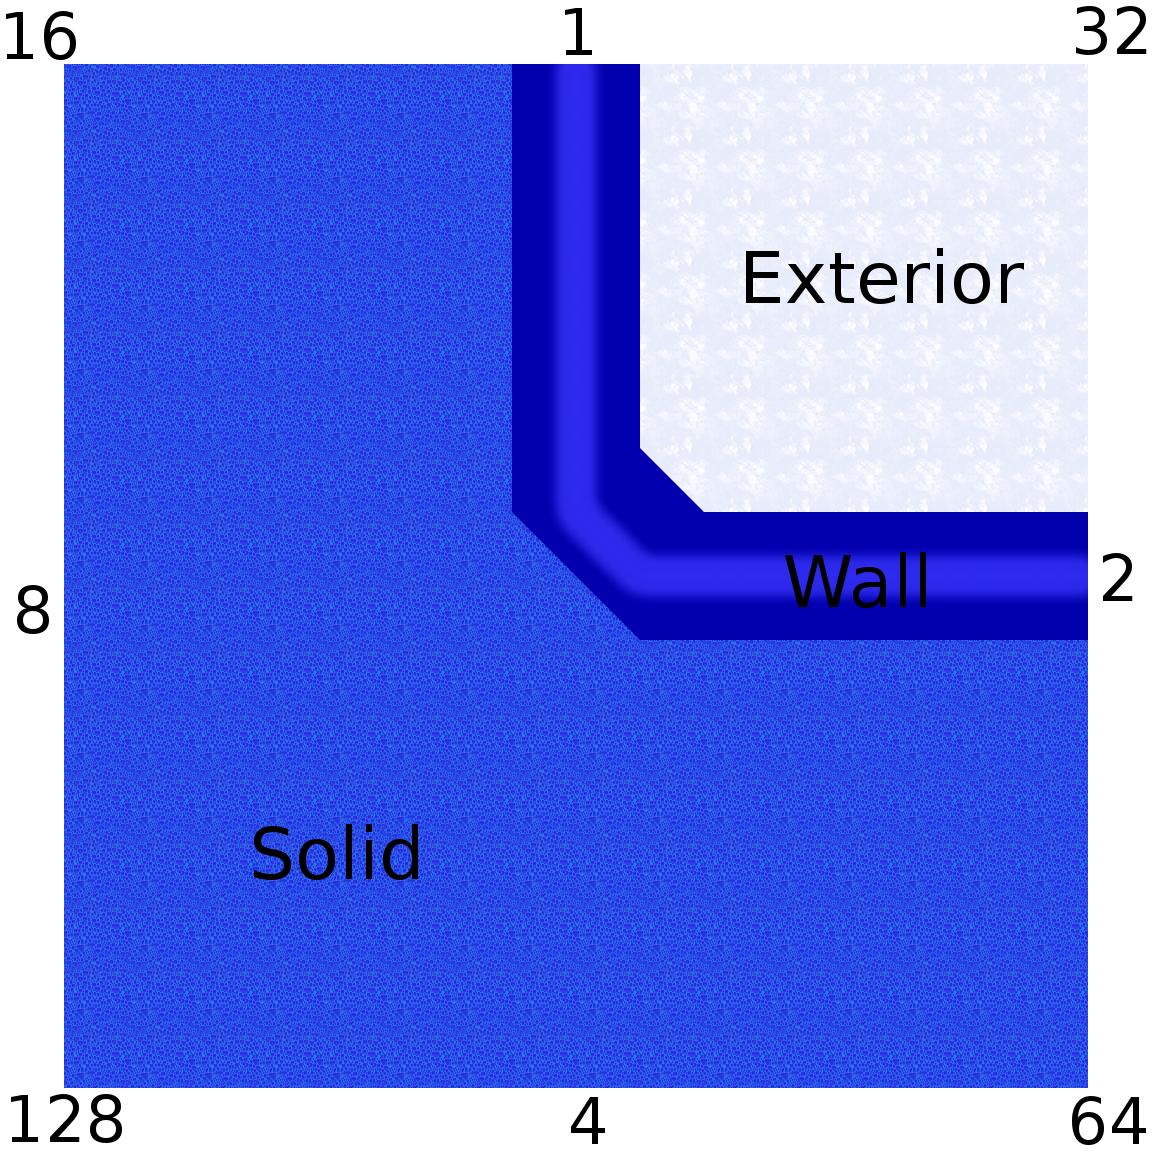
\includegraphics[width=3in]{WallSegment.png}
  \caption{Structure of a Typical Wall Segment}
  \label{fig:wall-segment}
\end{figure}

In order to have a standard way to classify the possible wall segments, we will use a shorthand code based on adding up the numbers in Figure \label{fig:wall-segment}.  

First, the wall itself.  There are four possible endpoints: up, down, left, and right.  A wall can have 0, 1, 2, 3, or 4 endpoints, as shown in Figure \label{fig:wall-endpoints}.  In order in this figure, these are none; up; up and right; up, left, and right; and up, down, left, and right.  Letting 1 mean up, 2 mean right, 4 mean down, and 8 mean left, we can assign a number from 0 to 15 to each possibility by adding the numbers of the endpoints used.  Thus, in order, the wall segments shown here are 0, 1, 1+2=3, 1+2+8=11, and 1+2+4+8=15.  

\begin{figure}[h]
  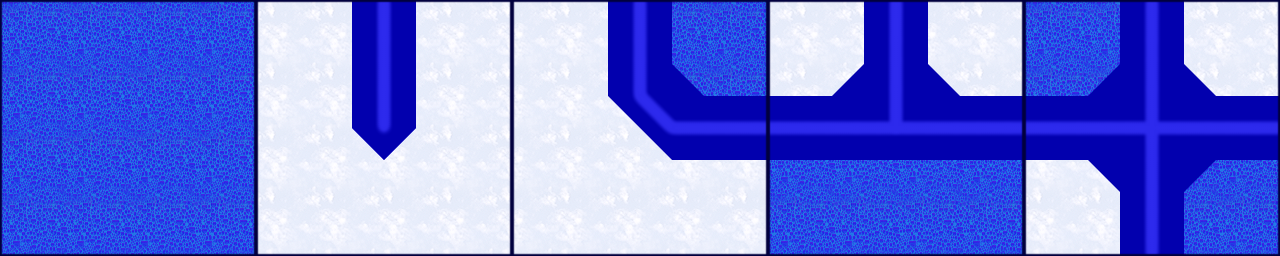
\includegraphics[width=3in]{WallEndpoints.png}
  \caption{Wall Endpoints}
  \label{fig:wall-endpoints}
\end{figure}

In addition, we have four possible locations for the solid, the top-left corner, the top-right corner, the bottom-right corner, and the bottom-left corner.  Numbering clockwise again, we let top-left be 16, top-right be 32, bottom-right be 64, and  bottom-left be 128.  We add the numbers of the regions that are considered ``solid'' for 15 possibilities.  Note that not all 15 possibilities actually happen for a given wall with endpoints.  In the figure, in order, the numbers are 240, 0, 32, 192, and 80. 

To find the code for a given wall segment, just add the solid code to the wall code.  Thus, in the figure, in order, the codes are 240, 1, 35, 203, and 95.  In Figure \ref{fig:wall-segment}, the particular segment shown has code $1+2+16+64+128=211$.

(It will be noted, it took the author multiple tries over several days to find a simple encoding scheme.  It is worth the effort to keep trying to find a scheme until a simple one is found, and not just go with the first idea that comes to mind.)

We thus have 256 possible wall segments, though many of them are not actually used.  This is a small enough number to create an array.

\subsection{Creating Wall Segments in GIMP}

The instructions here are but a suggestion, one of many possible ways to make walls that look good on the monitor.  The reader should feel free to modify and improve the walls at will.

\begin{task}[Exterior]
Open GIMP and create a new 256x256 image, transparency for background, and save it as ``WallSegments.xcf''. Turn on the grid (both showing and snapping to grid) and set the grid size to 32x32.  Rename the background layer ``Exterior'' and add two layers above it: ``Solid'', and above that one, ``Wall''.

Select the Exterior layer on the bottom and select the Paint tool, and select the Pattern Fill as the fill type.  Click the pattern icon box below the Pattern Fill and look for the sky pattern (light blue, and its name will be ``Sky'') and select that.  Adjust the Opacity (the default is 100\%) and change it to 25\% so the pattern is not quite so strong.  Click in the image to fill the Background layer with sky.  This will be our ``exterior''.
\end{task}

Now, everything we do will go on top of this exterior.  Next we create four regions for the solid portion of the wall.

\begin{task}[Solid]
Select the Solid layer.  Right-click it and select ``Duplicate Layer''.  Do this 3 more times to create 4 solid layers.  Rename them SolidTL, SolidTR, SolidBR, and SolidBL.

Select the SolidTL layer.  Then use the Rectangle Select tool and use the grid to help you select the top-left quarter of the image.  Select the paint bucket tool and change the pattern to Blue Web (a darker blue than the sky).  Change the opacity back to 100\% to make it truly solid. Then click in the selection to paint the top-left quarter of the layer.  See Figure \ref{fig:top-left-solid}.

Now select the SolidTR layer and follow a similar procedure to fill the top-right quarter with the blue web pattern.  (Note, you can click on the ``eye'' icon next to a layer to hide, or reveal, the layer; this can make it easier to work on individual layers.)

Do this again twice more, for the SolidBR and Solid BL layers.  Then test that you can click the eye icons to make whatever pattern of solid you need.  When done, click the Eye icons to hide these four layers so we can work on the walls.
\end{task}

\begin{figure}[h]
  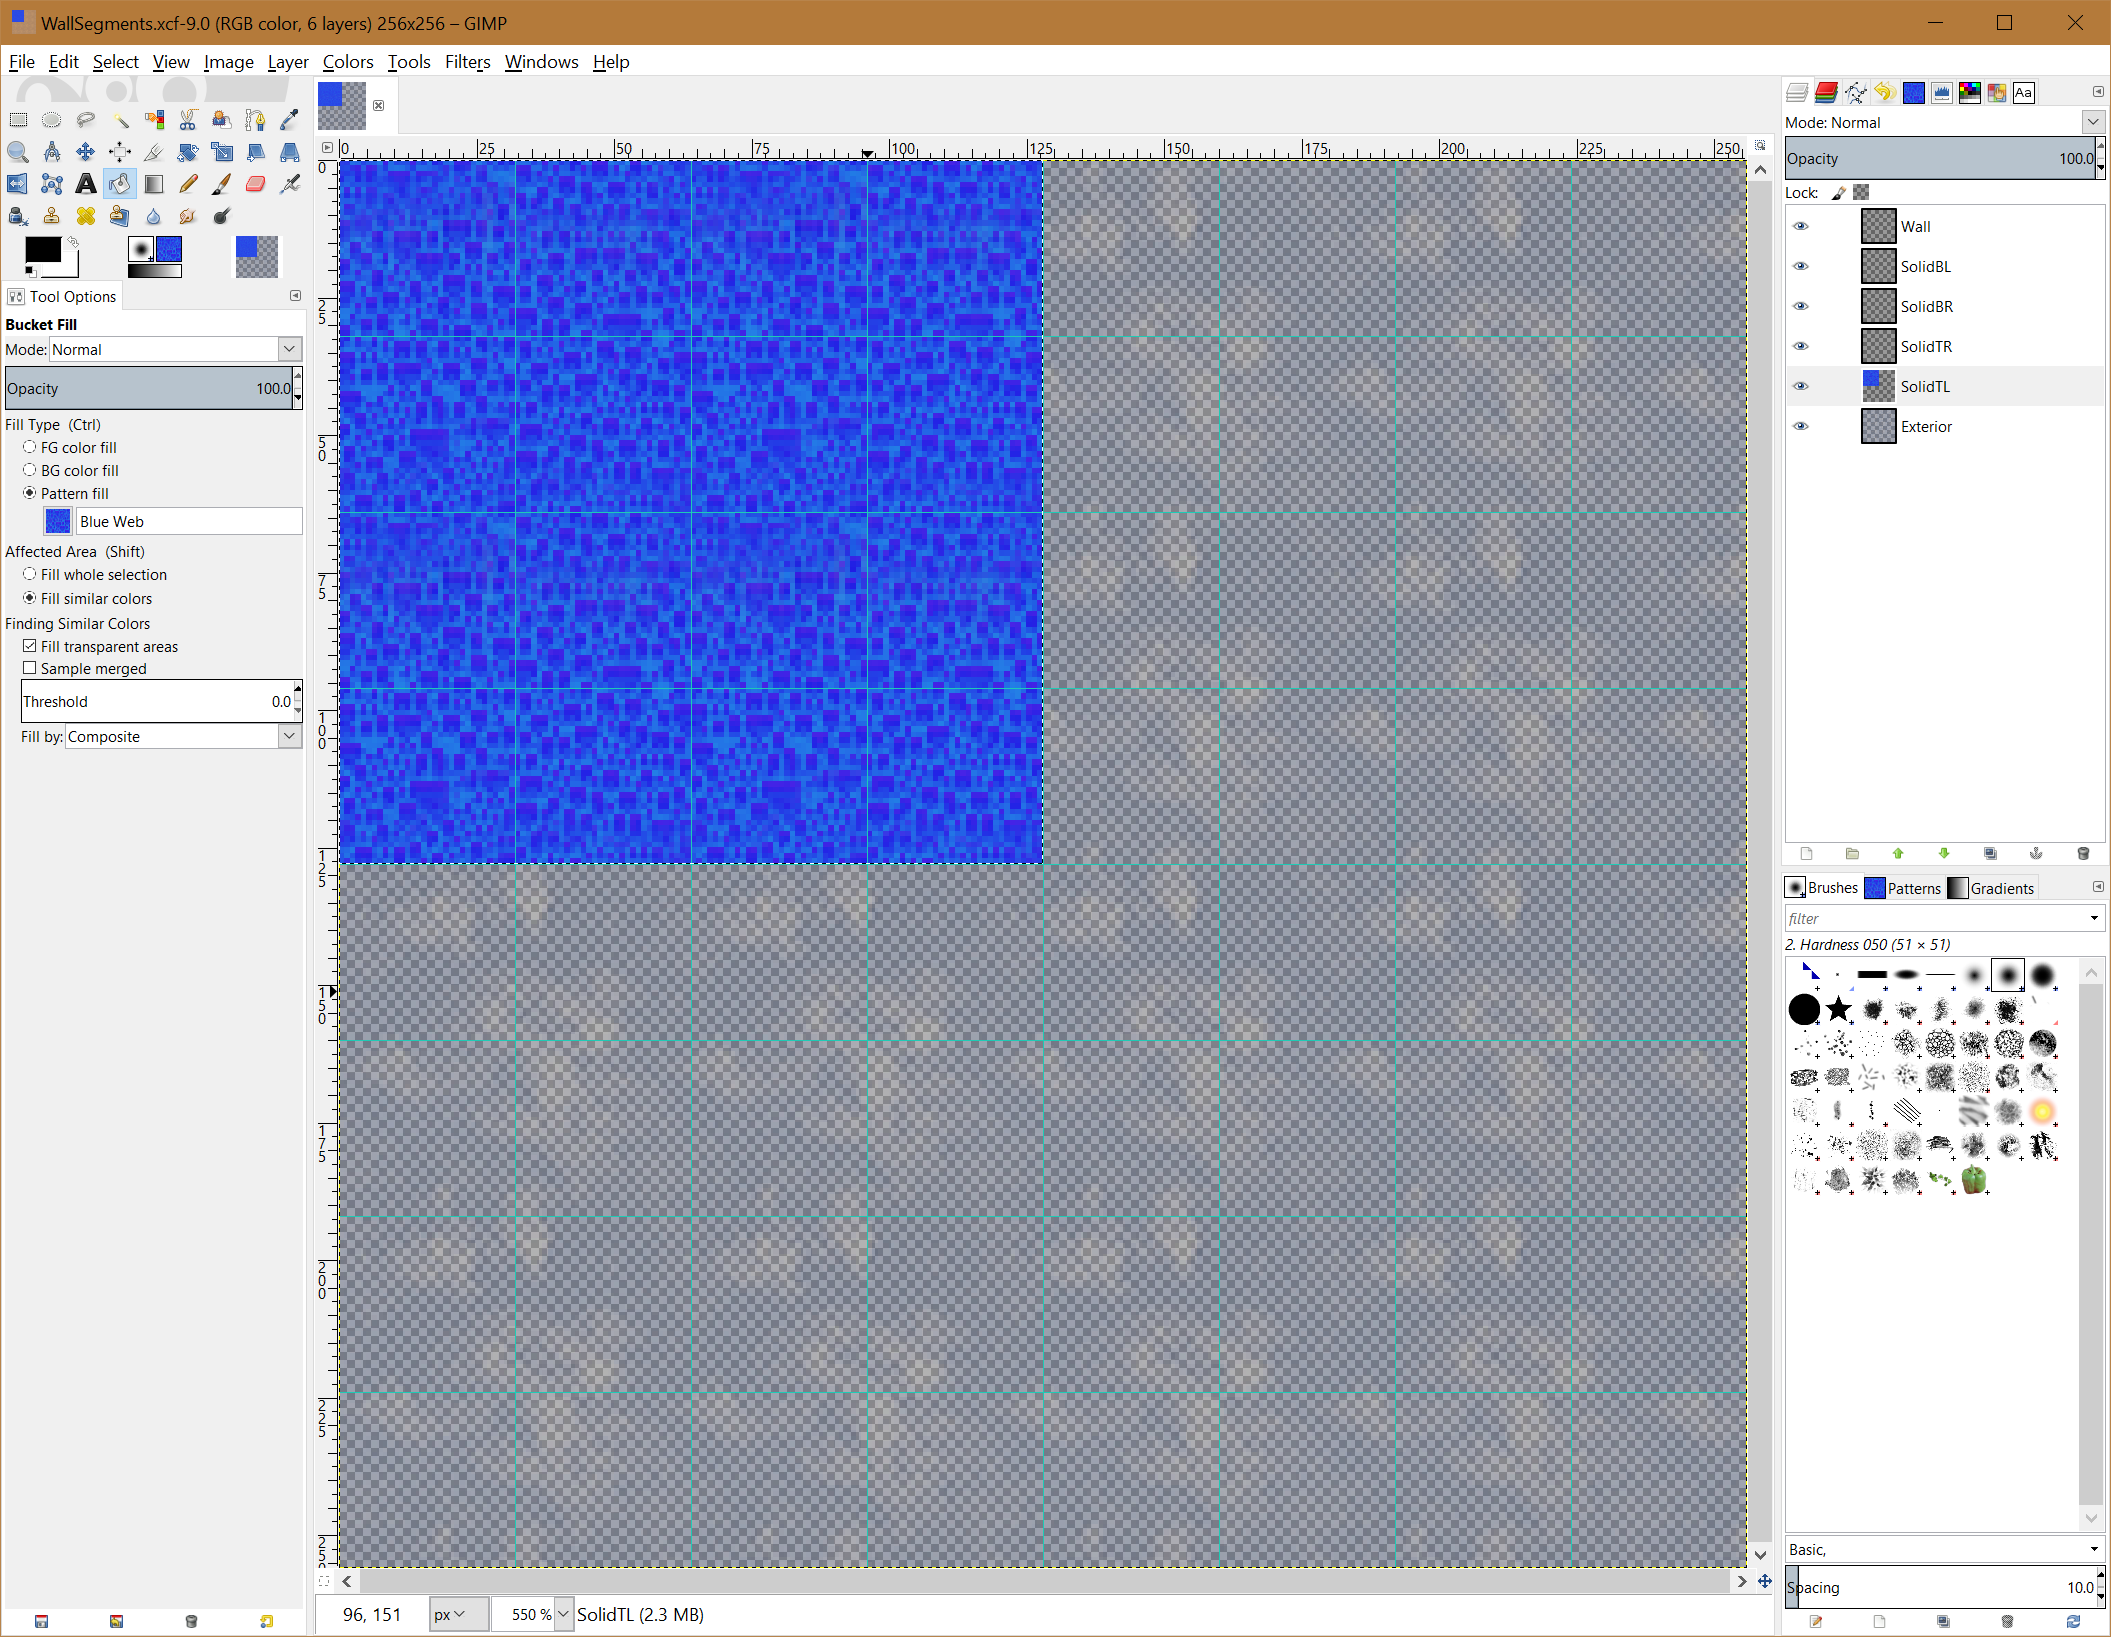
\includegraphics[width=3in]{TopLeftSolid.png}
  \caption{Creating the Top Left Solid region}
  \label{fig:top-left-solid}
\end{figure}

\subsection{Build a Wall}
Let us build a wall.

\begin{figure}[h]
  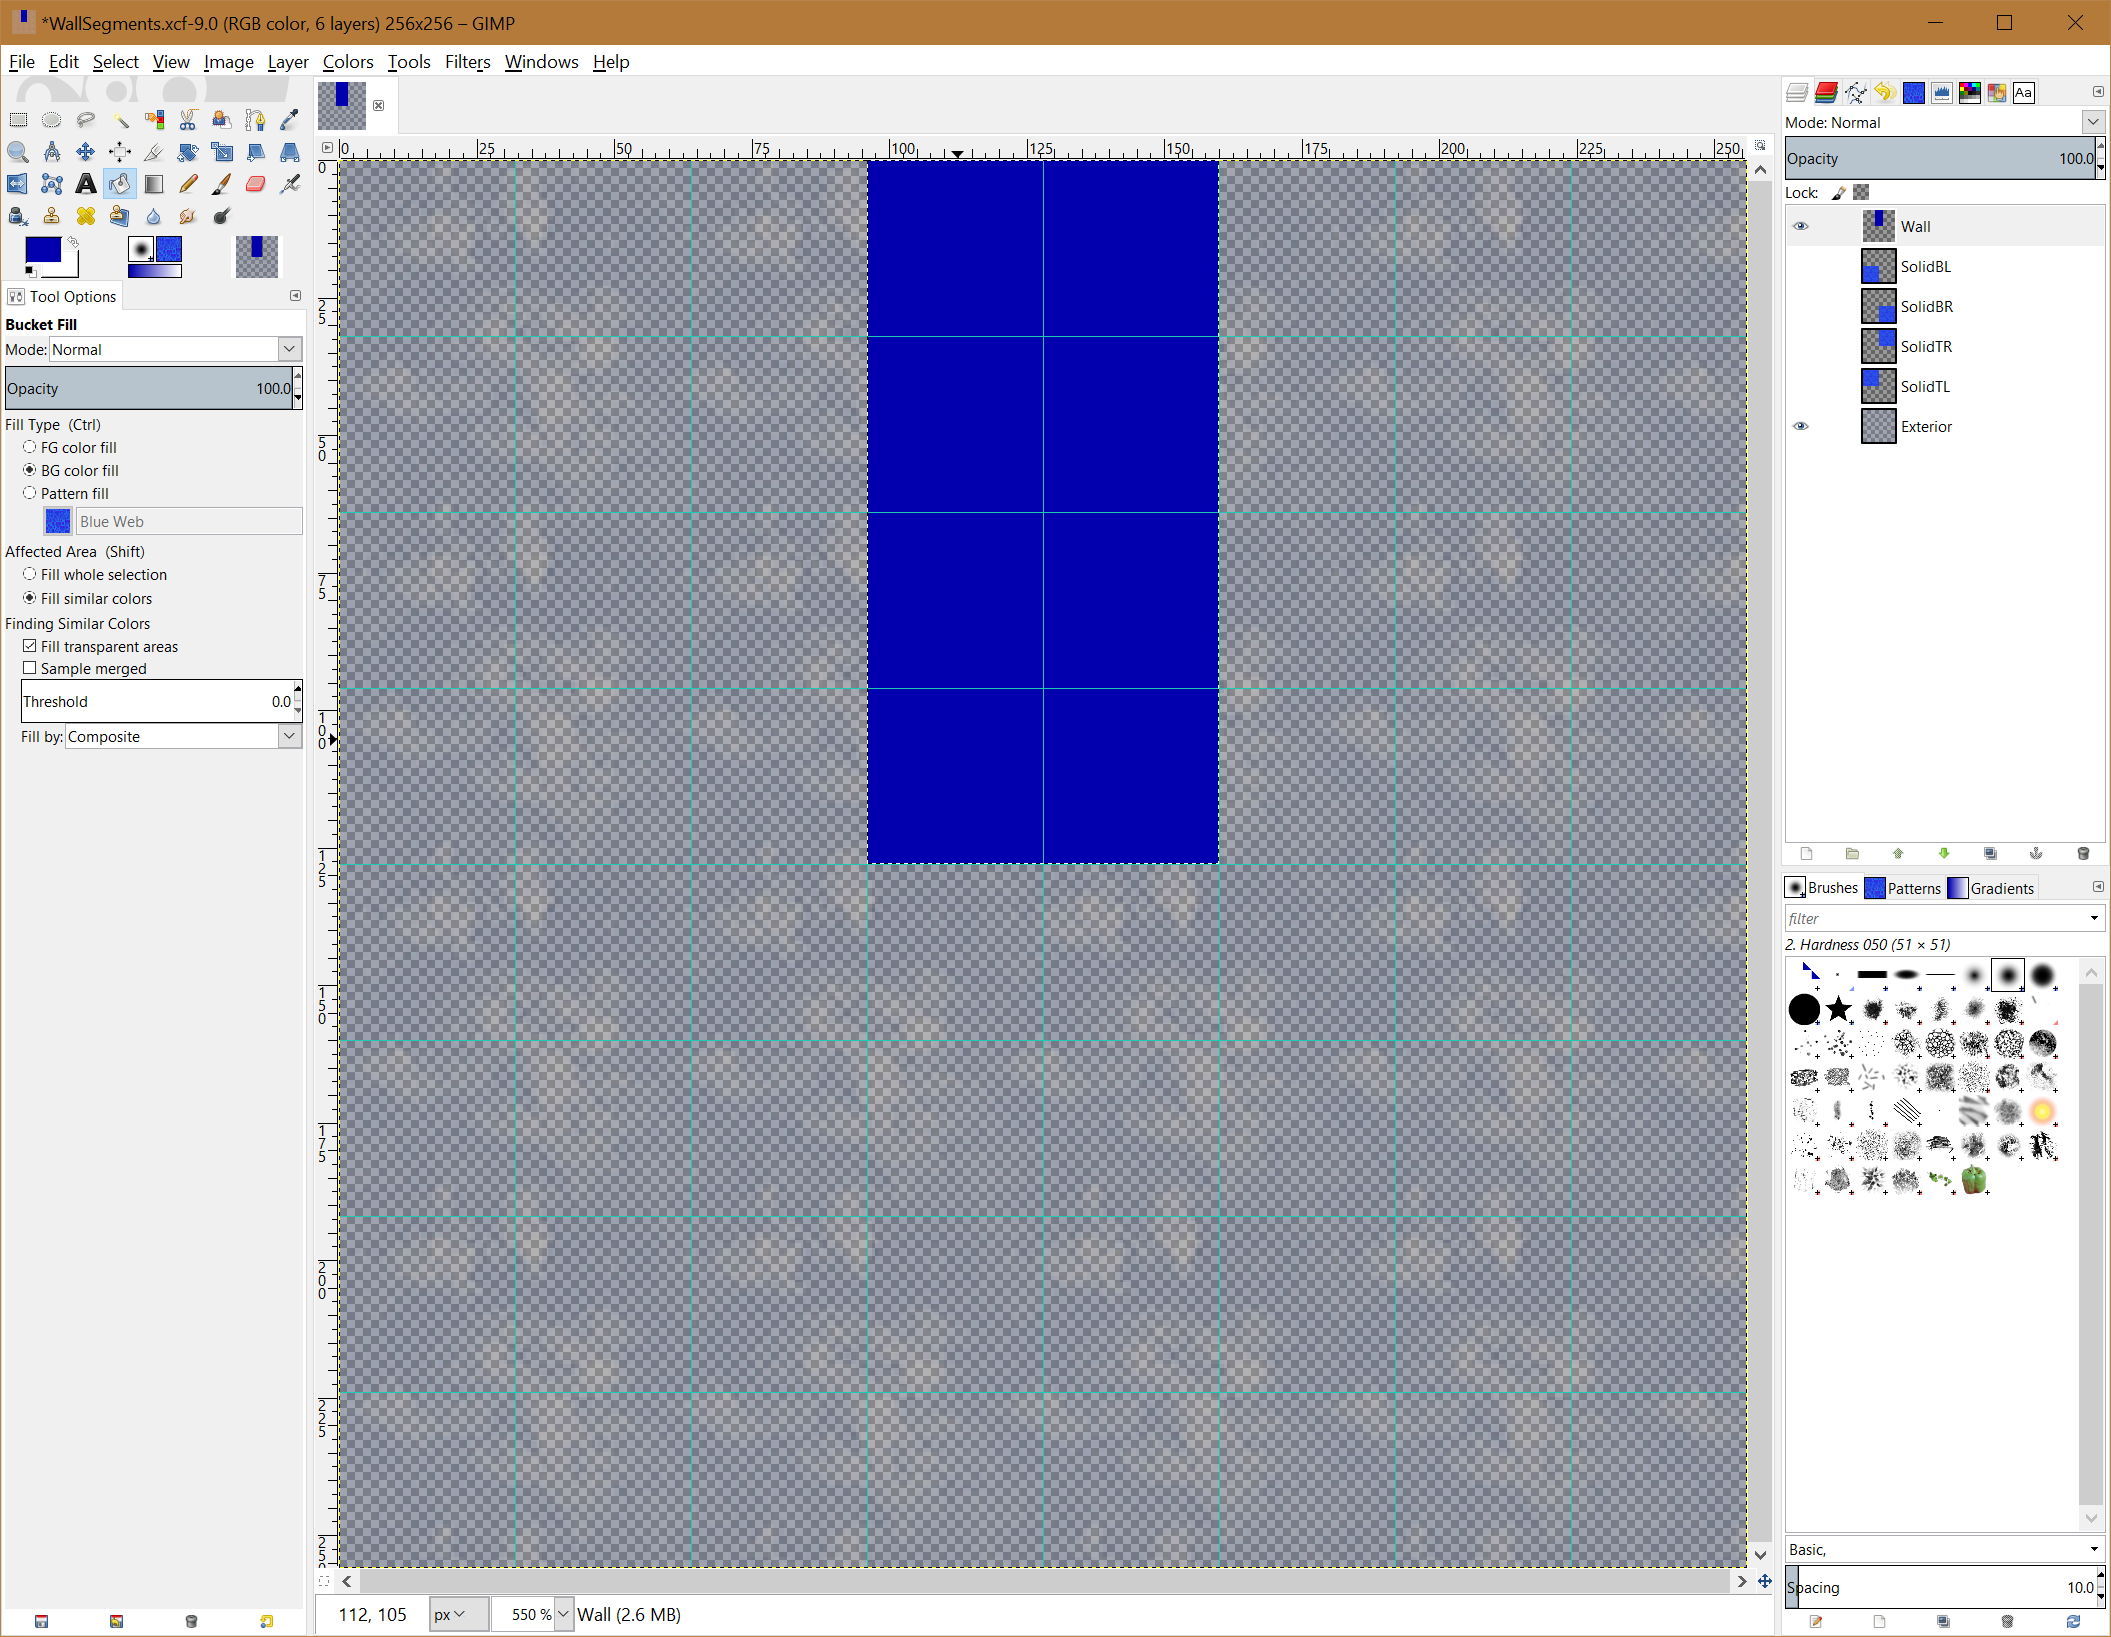
\includegraphics[width=3in]{UpWall.png}
  \caption{Creating the Up-to-center Wall}
  \label{fig:up-wall}
\end{figure}
  
\begin{task}[Wall]
Select the Wall layer.  Let us make our first wall to be the code 1 wall (endpoint is ``up'', and it ends in the center of the tile).  

For the most basic possible wall, use the grid to help draw a rectangle 64 pixels wide by 128 pixels long from the top middle to the center of the tile.  Set the paint bucket tool to Foreground Color Fill and change the foreground color to a dark blue (hex 0200ae).  Click the rectangular section to make a very basic up-to-center wall (Figure \ref{fig:up-wall}).

We could stop there, but we can do better.  Let us put an end-cap on that wall to make it look nicer.  Select a triangle, using the Lasso select tool and clicking on the three triangle vertices, and fill it with the same dark blue (Figure \ref{fig:endcap}).  Clear the selection using the Select menu, the None choice.

We could stop here, but we can do better still.  Let us make the wall look something like a Jersey wall viewed from above and put a ridge on it.  Select the paintbrush tool.  Select a brush with a hardness of 50\%.  Make sure opacity is 100\%.  Make sure the size is 20.  Change the foreground color to a slightly lighter blue (hex 2d2aed).  Click the top middle of the wall rectangle, and holding down shift, click the center of the tile, thus drawing a line from the top middle of the rectangle down to where the rectangle transitions to the endcap.  See Figure \ref{fig:wall-complete}.
\end{task}

\begin{figure}[h]
  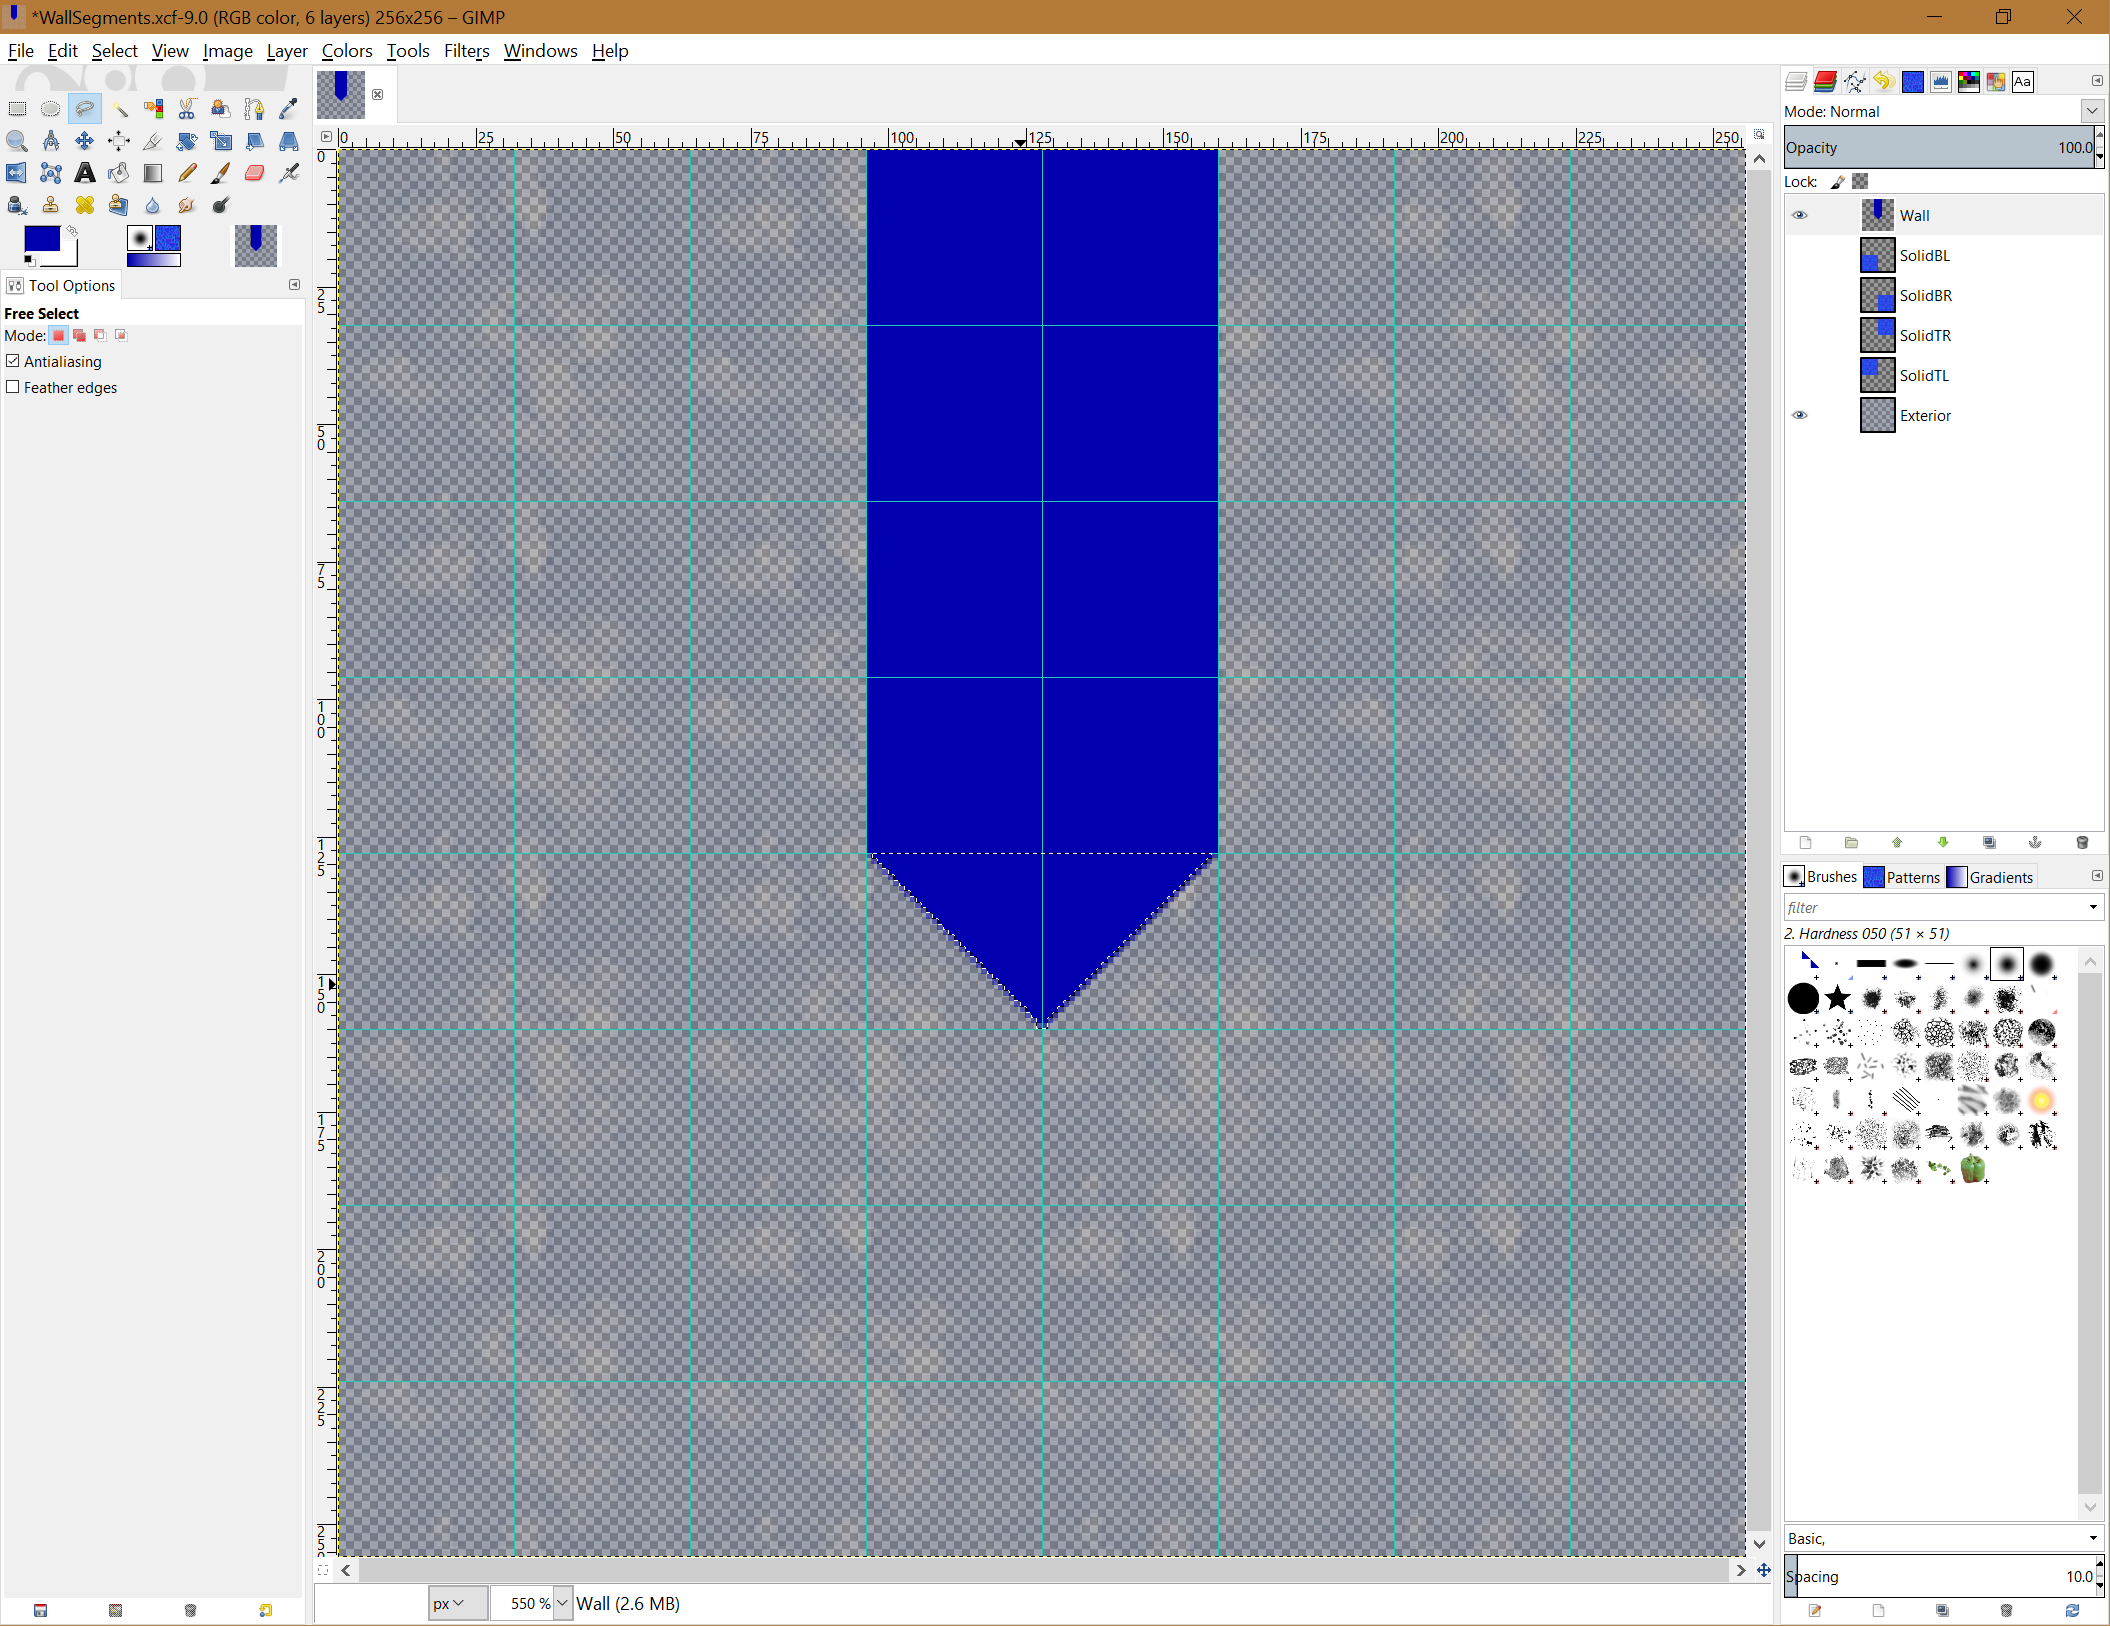
\includegraphics[width=3in]{EndCap.png}
  \caption{An Endcap Makes the Wall Look Nicer}
  \label{fig:endcap}
\end{figure}


\begin{figure}[h]
  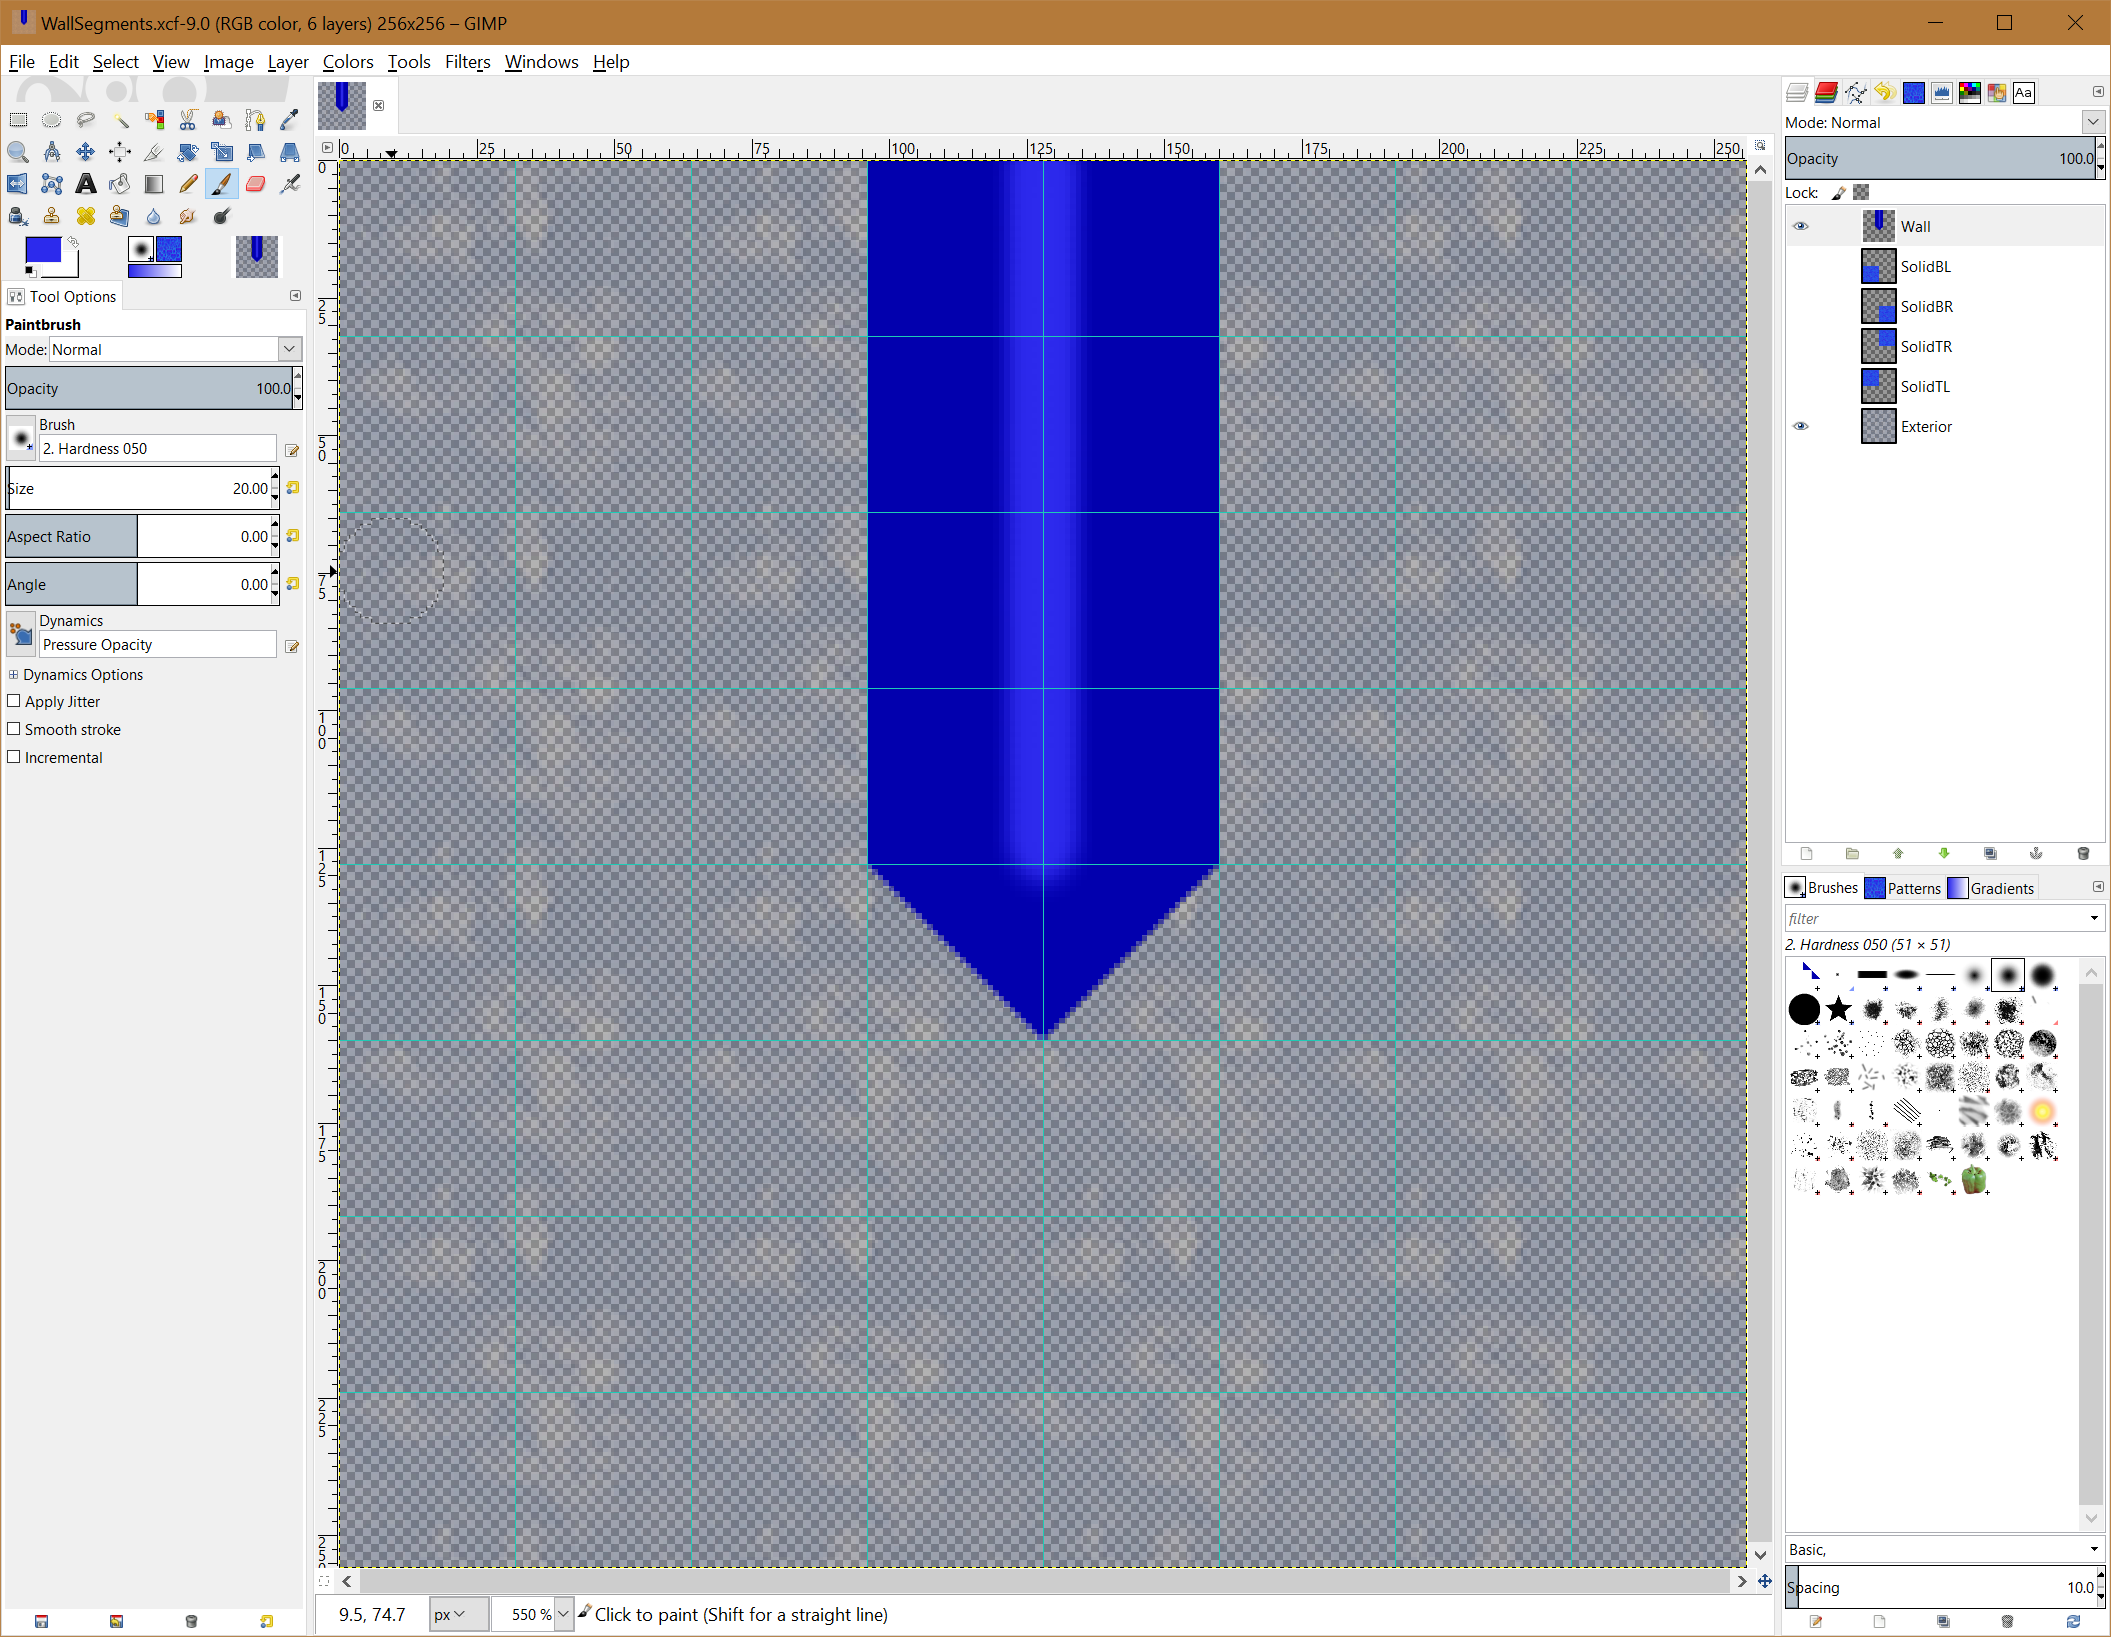
\includegraphics[width=3in]{WallComplete.png}
  \caption{A Ridge Improves the Wall Even More}
  \label{fig:wall-complete}
\end{figure}

\begin{task}[Three More Walls]
Now that we have the up-only wall of code 1, we can make the right, down, and left walls with codes 2, 4, and 8, respectively.  To do this, duplicate the Wall layer and use the Layers menu (not the Image menu which has similar options) Transform option and the rotate 90 and 180 choices.  Rename the four wall layers as WallUp, WallRight, WallDown, and WallLeft appropriately.  Use the Eye icons to hide and reveal walls to ensure they all look OK.
\end{task}

We will make a vertical and horizontal wall now, using the walls we have already created.

\begin{task}[Straight Walls]
In the layers panel, use the eye icons to hide all the wall layers and the solid layers, leaving only the Exterior layer.

Create a new layer and name it WallUpDown.  Using the same methods as before, draw a dark blue rectangle 64 pixels wide and going from the top to the bottom of the tile, centered from left to right.  Note that the same dark blue used before should be in the pallet of the foreground color selector, so it can be reused.

There is no endcap for this wall, but it still has a ridge.  Change the foreground color to the lighter blue used before and select the paintbrush tool, with the same settings as before.  Draw the ridge by clicking on the top middle edge of the tile, and then with the shift key held down, the bottom middle edge of the tile, to create a vertical ridge down the center.

Duplicate this layer and rename it WallLeftRight. Use the Layers menu Transform to rotate it 90 degrees.
\end{task}

\subsection{Corner Walls}
Let us make the up-right corner wall and leave the other three as an exercise.


\begin{figure}[h]
  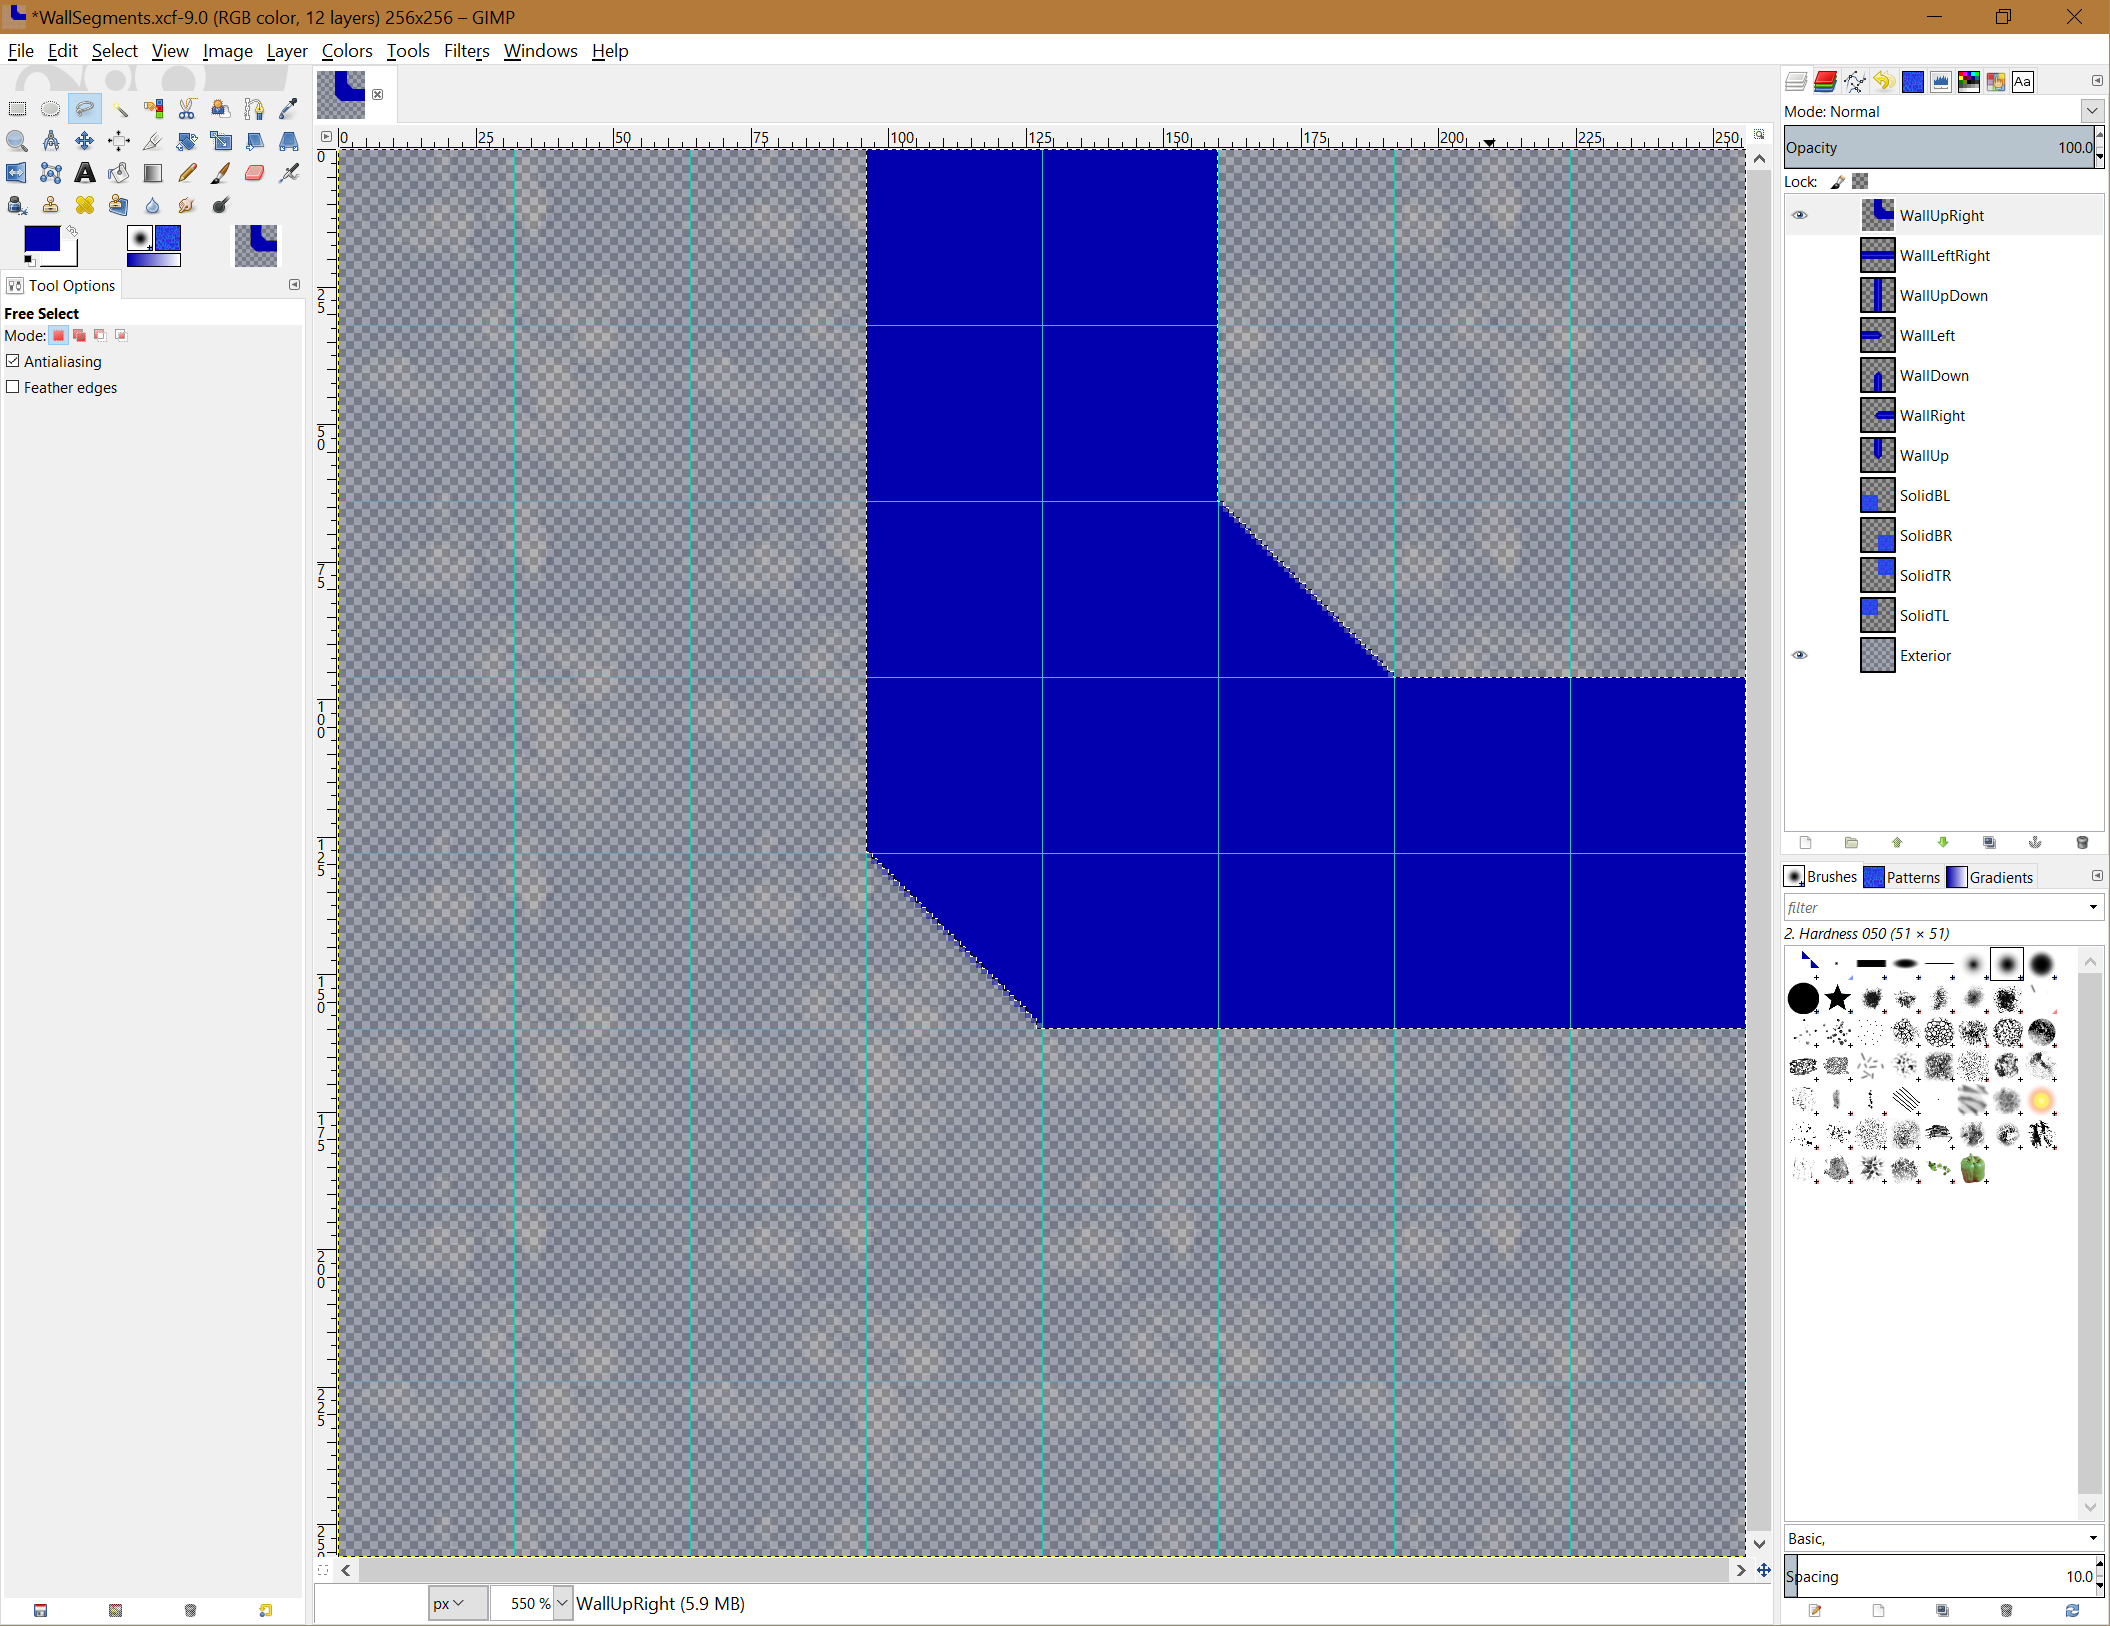
\includegraphics[width=3in]{WallUpRight.png}
  \caption{Selection for Up Right Wall}
  \label{fig:up-right-select}
\end{figure}


\begin{task}[Up Right Corner Wall]
With all walls and solid regions hidden, create a new layer called WallUpRight and make sure it is the selected layer.

Use the Lasso select to select a polygon like that in Figure \ref{fig:up-right-select}, and fill it with the same dark blue as before.

With the paintbrush tool and the lighter blue used before, draw the ridge like in Figure \ref{fig:up-right-finish}.
\end{task}

\begin{figure}[h]
  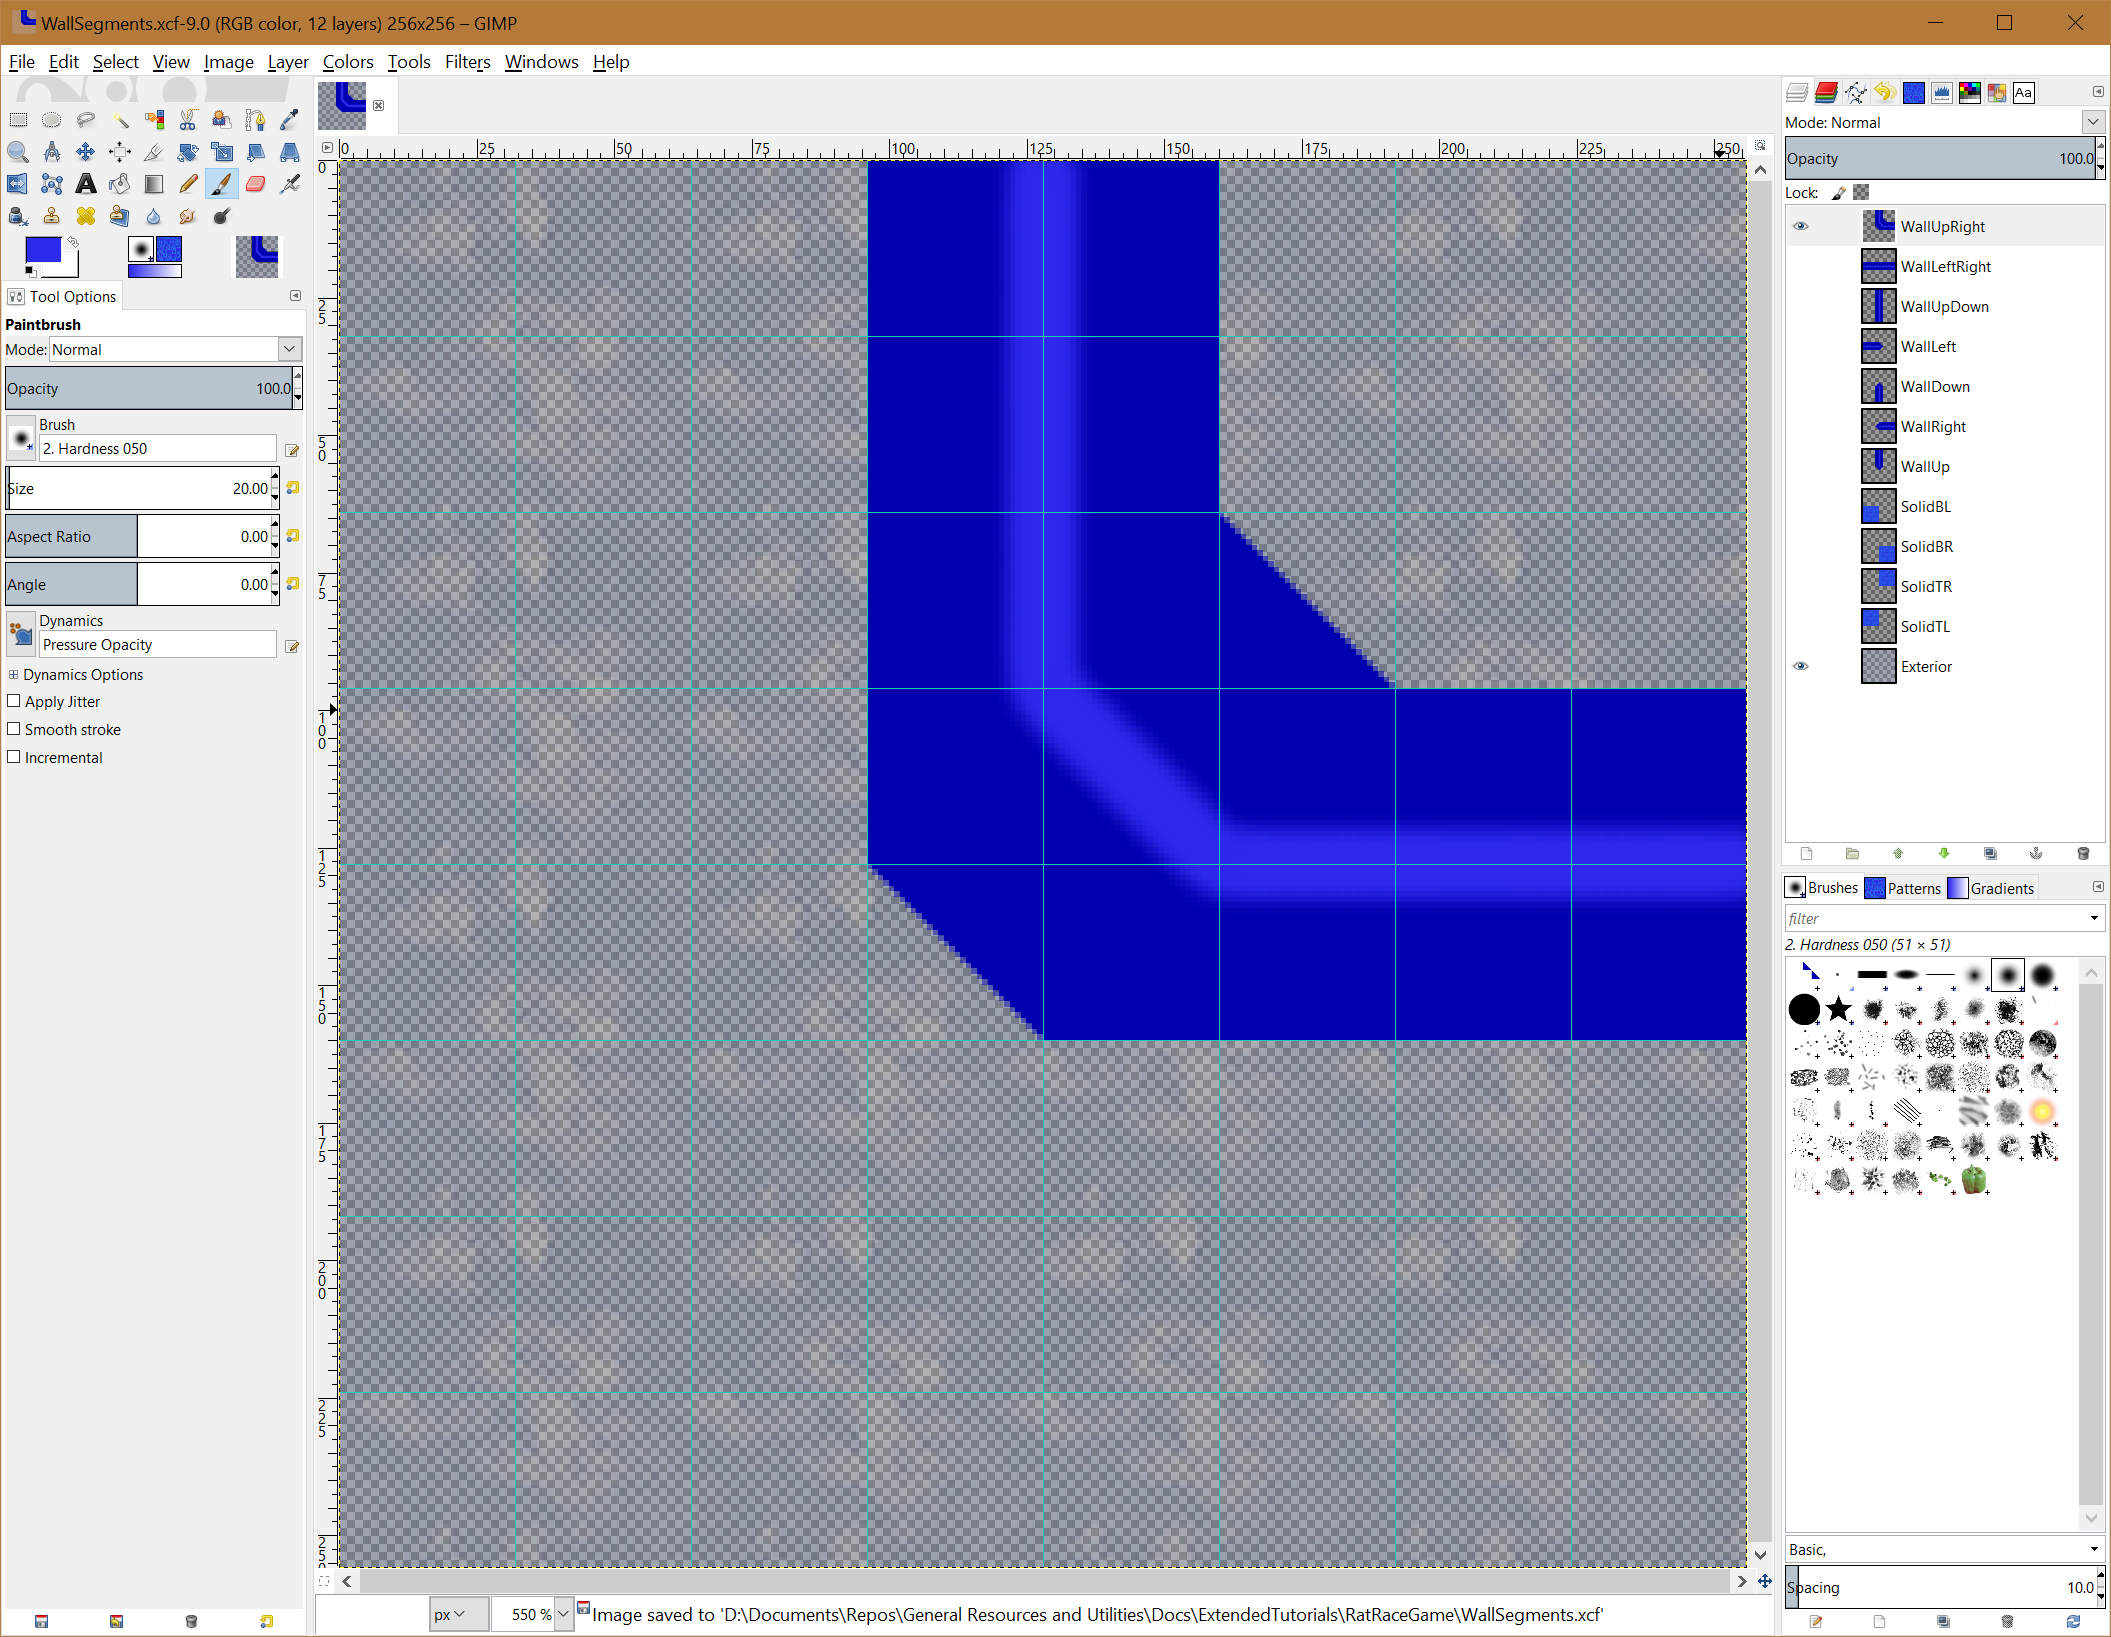
\includegraphics[width=3in]{WallUpRightComplete.png}
  \caption{Ridge for the Up Right Wall}
  \label{fig:up-right-finish}
\end{figure}

\begin{exercise}
Complete the Up Left Wall, the Down Right Wall, and the Down Left Wall, either the same way as for the Up Right wall or by copying and rotating layers.  Name the layers appropriately.
\end{exercise}

\subsection{Remaining Wall Segments}


\begin{figure}[h]
  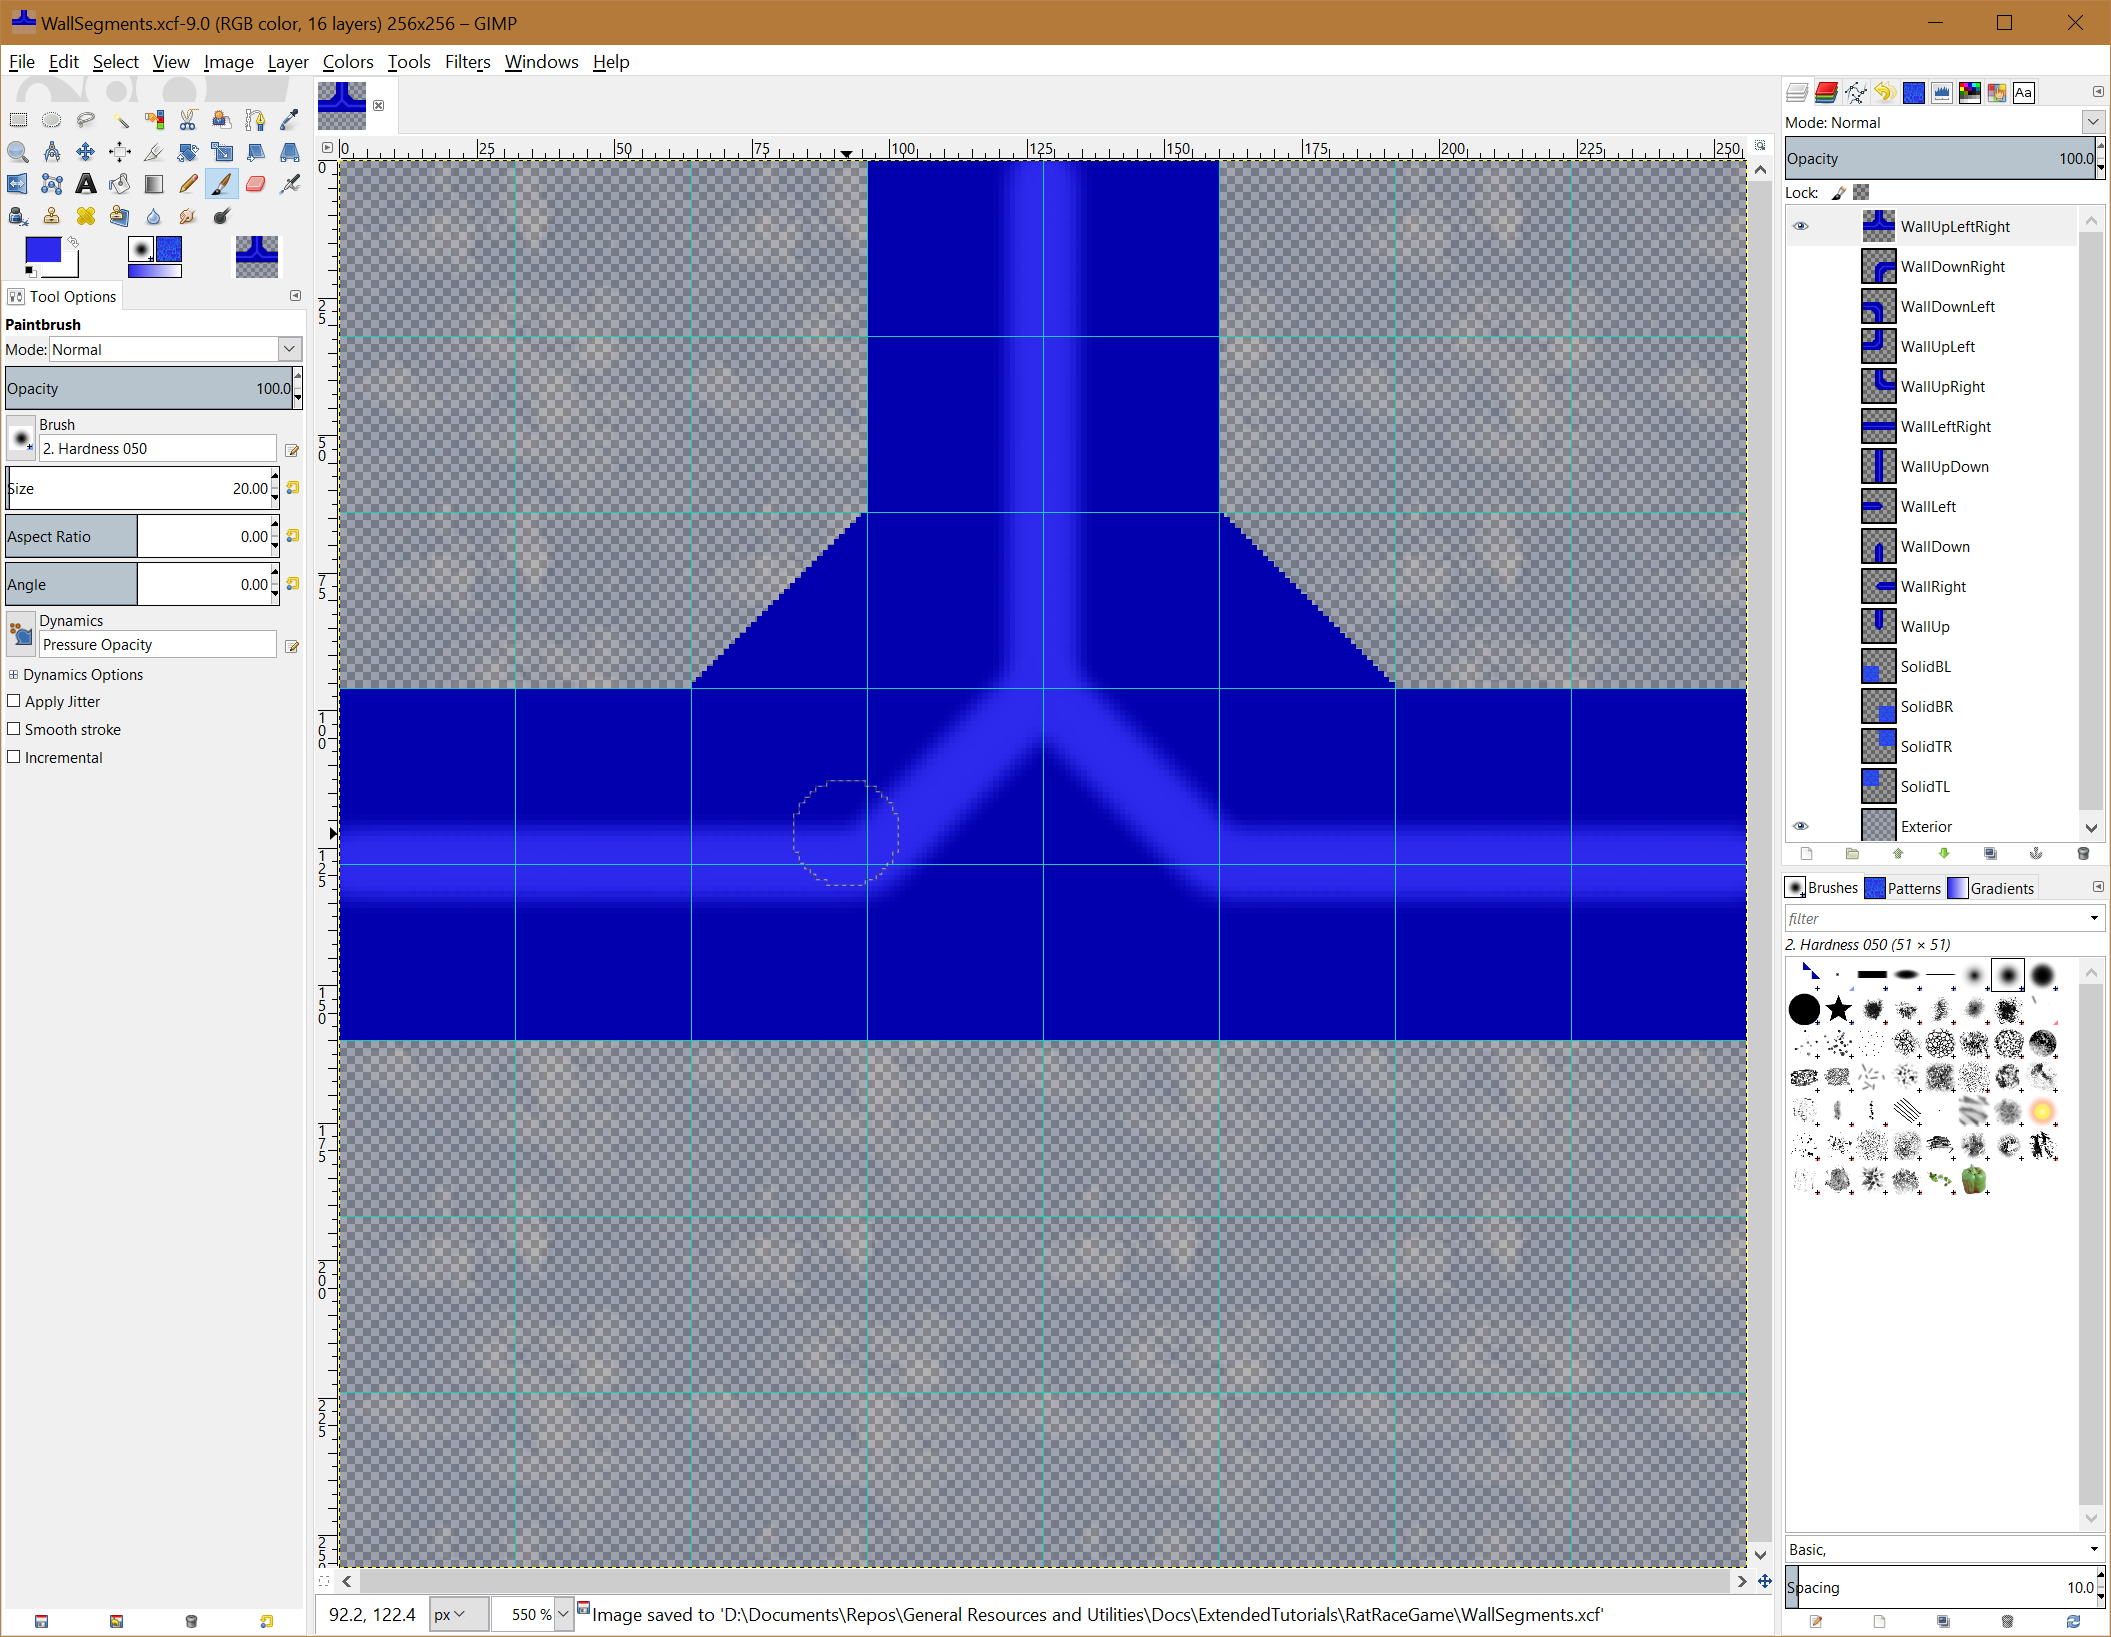
\includegraphics[width=3in]{Tee.png}
  \caption{A Tee Wall (Up Left Right)}
  \label{fig:tee}
\end{figure}

\begin{exercise}
Using the above procedures and Figure \ref{fig:tee} as a guide, create the four tee walls: with endpoints up, left, right; right, up, down; down, right, left; and left; down, up.  
\end{exercise}


\begin{figure}[h]
  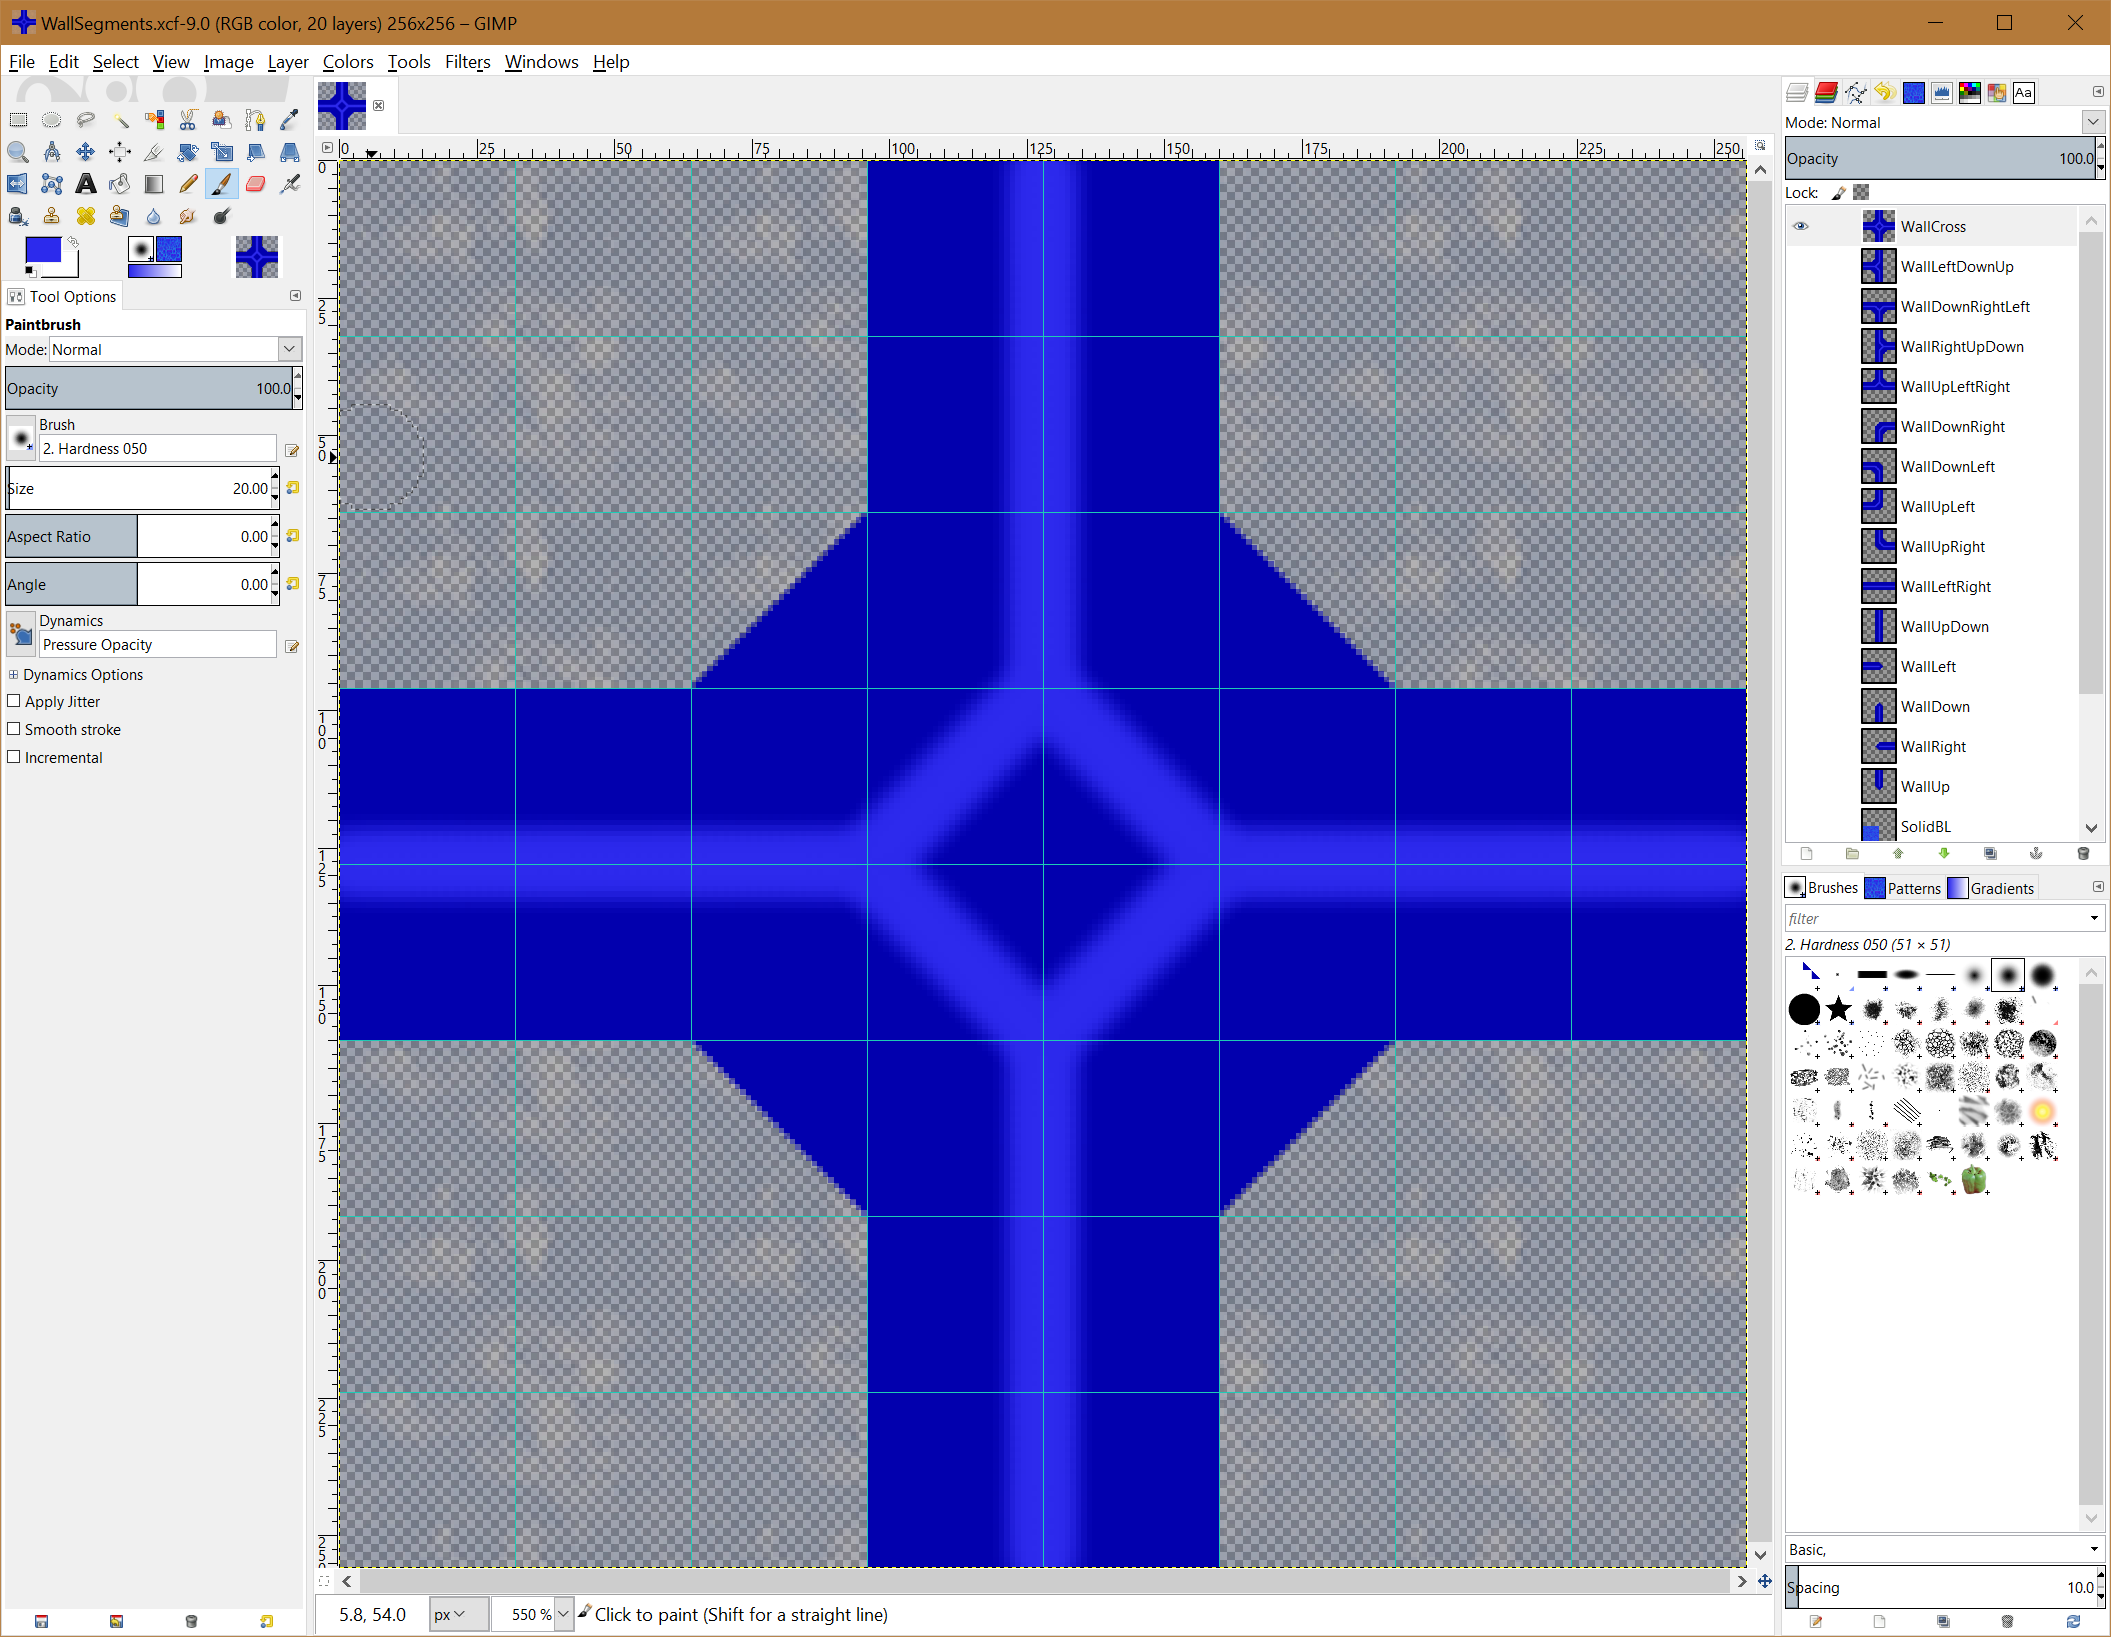
\includegraphics[width=3in]{Cross.png}
  \caption{A Cross Wall (Up Down Left Right)}
  \label{fig:cross}
\end{figure}

\begin{exercise}
Using the above procedures and Figure \ref{fig:cross} as a guide, create the cross wall: with endpoints in all four directions.
\end{exercise}

Make sure the file is saved.  This file has all the parts needed to build our walls.

\chapter[Improving Maze Walls II]{Improving the Maze Walls II: Building the Maze}

Before we can use the wall sections to build the maze, we have to import them into our Unity project.

\begin{task}
In GIMP, in the WallSegments file, make sure the Exterior layer is showing, and hide all other layers.  This can be done quickly by holding down the Shift key and clicking the eye icon of the layer (possibly twice).  With the Exterior layer being the only layer visible, export it to a file called ``Exterior.png''.  This can be done using the keyboard shortcut Ctrl-Shift-E (or CMD-Shift-E on a mac).  Make sure you save it in the Unity project Rat Race in the Assets folder under Sprites.  

Then do the same with the next layer up (SolidTL if you followed the directions the same order the author did).  Show that layer and only that layer, and export it to a file with the name SolidTL.png in the same directory that the Exterior.png file was saved to.

Do this for the remaining 18 layers.
\end{task}

Note that there is a 3rd party plugin that can do this automatically.  It is optional if a user wishes to use this.  For just 20 layers, and just one time, the one-at-a-time method works fine, though.

After you have exported 5 or 6, you might want to go to Unity and make sure these are importing ok before continuing.  Optionally, create a Walls folder in the Sprites folder and move all the wall sprites there.  Then when you go back to GIMP, continue exporting into the Walls directory.

When done, look over the sprites in Unity (Figure \ref{fig:import-wall-segments}).  Note that in the Projects panel, in the folder holding the sprites, if you move the slider at the bottom right of the panel all the way to the right, large thumbnails of the sprites will be shown. Check for missing exports or exports that did not go right (for example, if you accidentally had more than one layer showing when exporting one of the sprites) and re-export them from GIMP.  If you notice a name spelled wrong, it can be corrected here.

Now, select all of the sprites (Shift-click or Ctrl-click or CMD-click) and look at the settings in the Inspector.  Change the Pixels Per Unity property to 256 and click the Apply button.

\begin{figure}[h]
  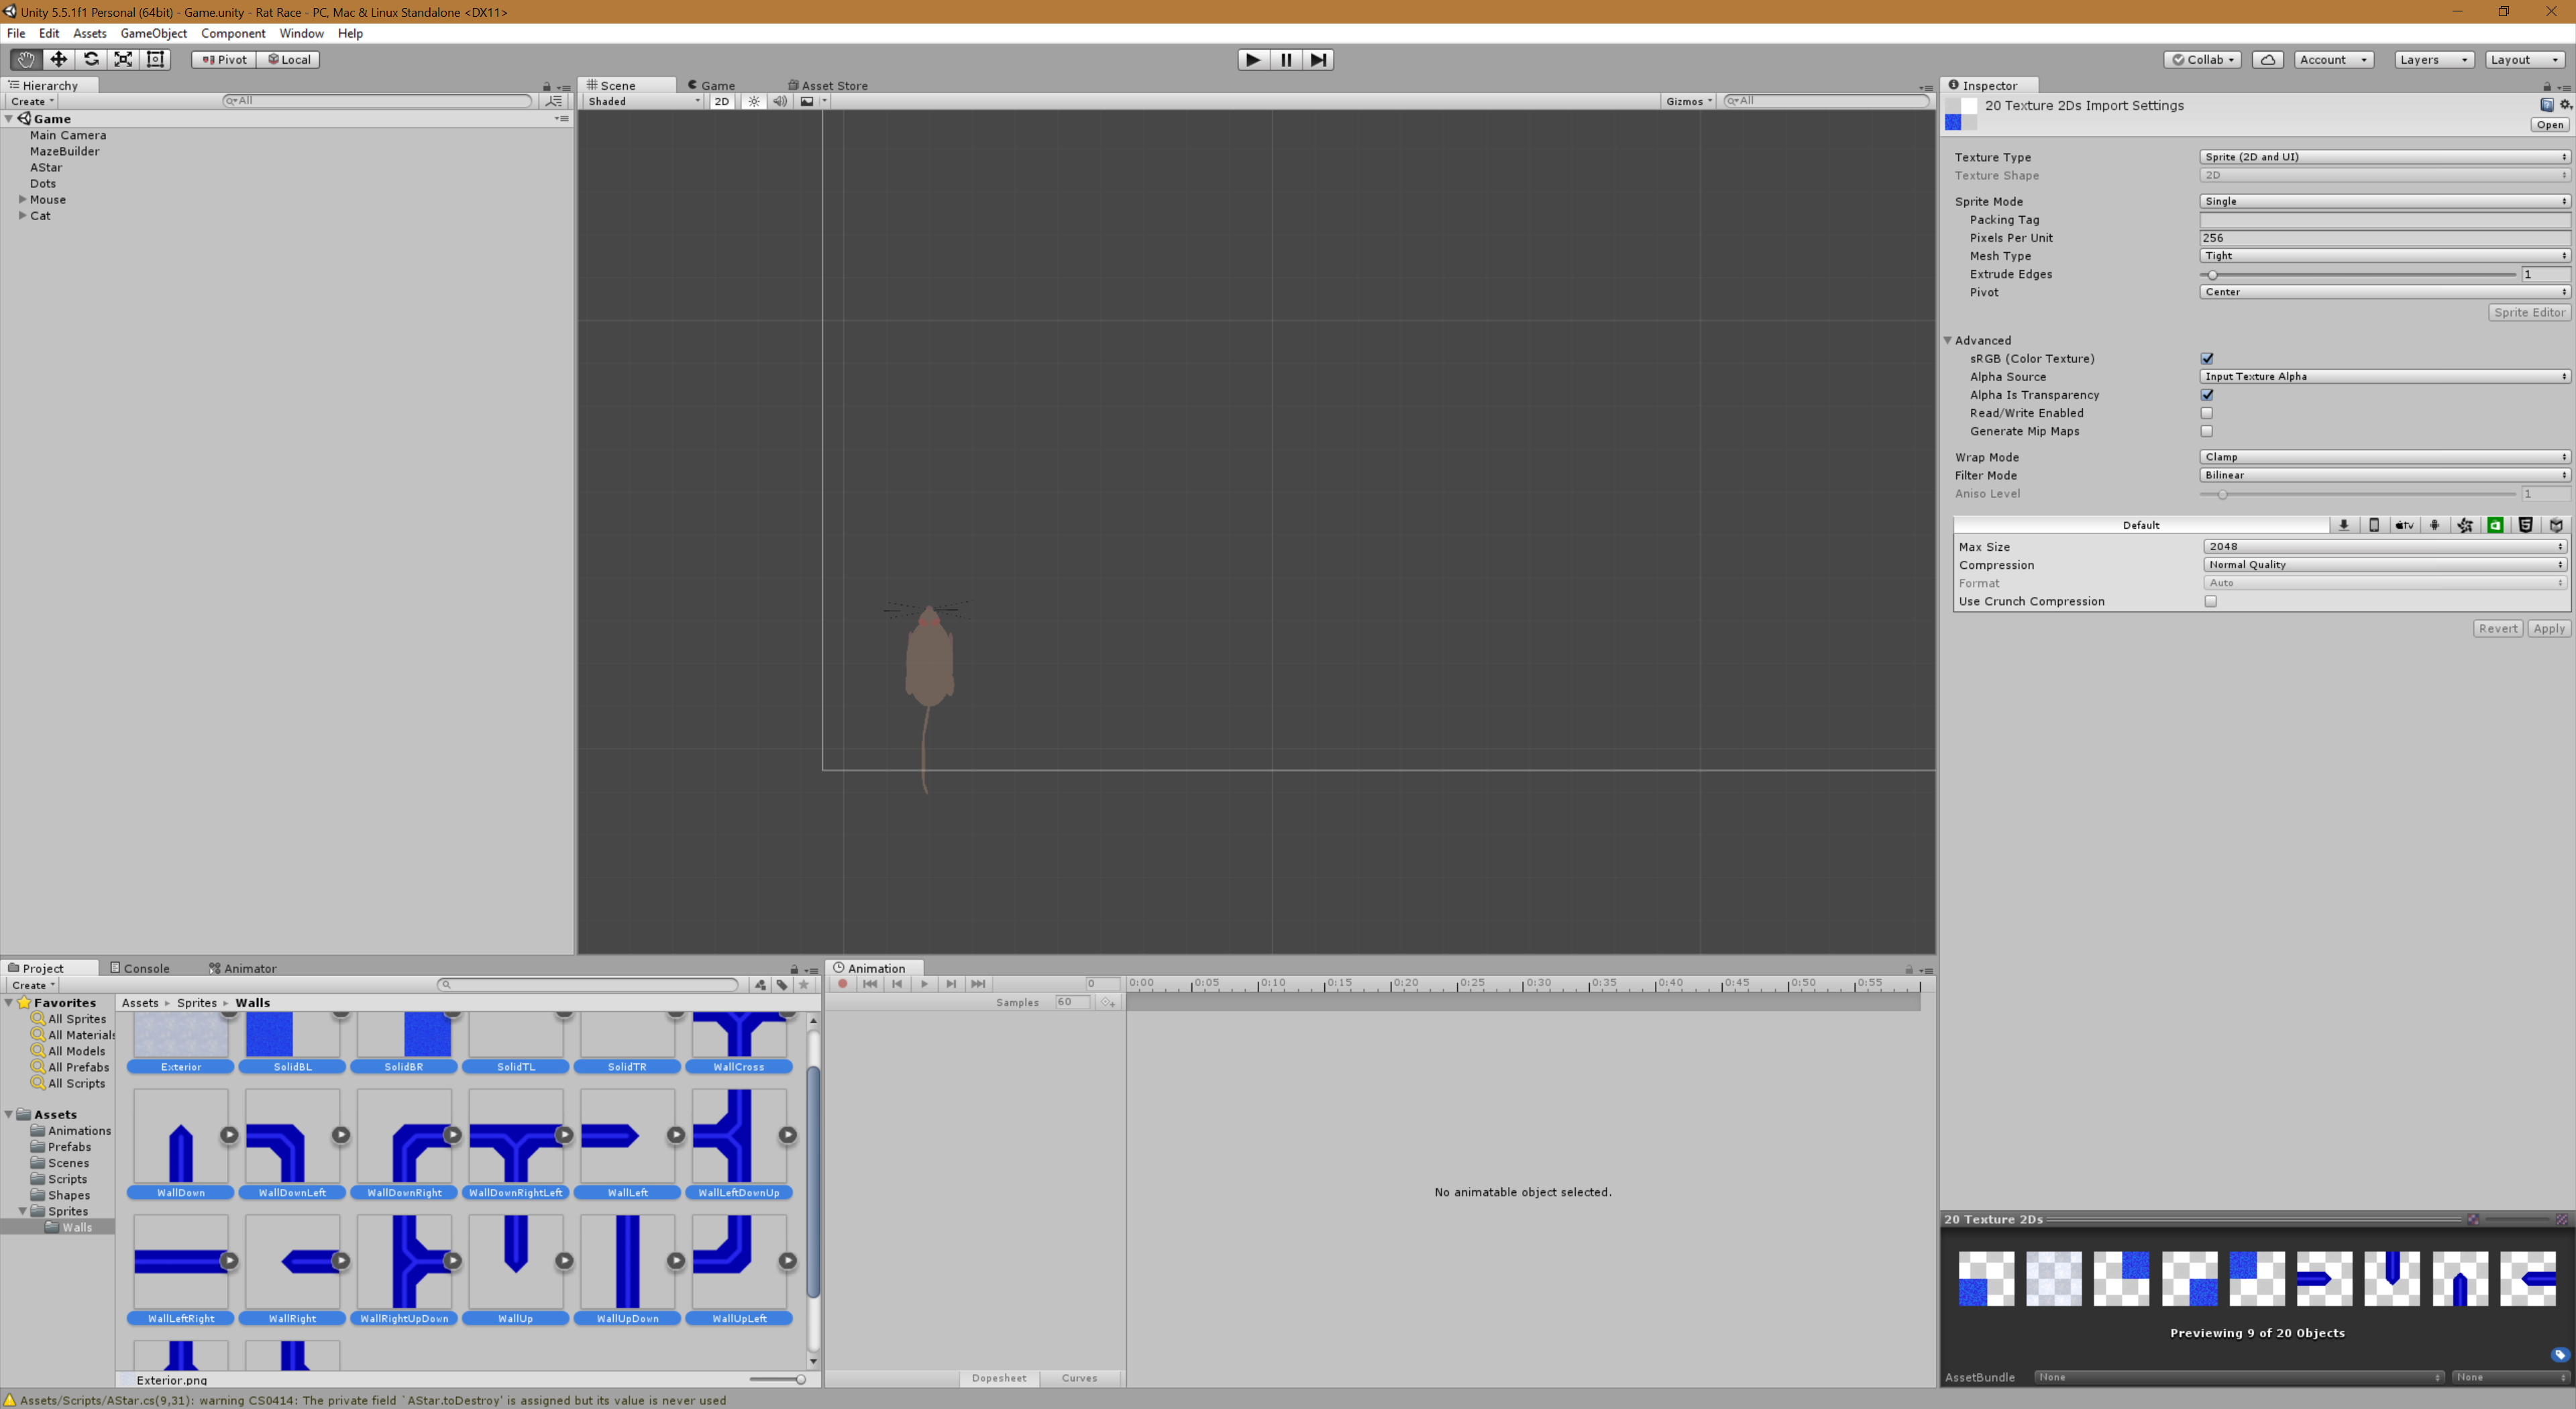
\includegraphics[width=6in]{ImportWallSegments.png}
  \caption{Wall Segments Imported into Unity}
  \label{fig:import-wall-segments}
\end{figure}


\subsection{Modifying the MazeBuilder Script}
We divide the new wall segments into three types: the single Exterior tile, the four solid regions, and the 15 wall tiles.  Let us first create two arrays and one variable in the MazeBuilder script to hold these tiles.

\begin{task}
Add these lines to the MazeBuilder \csharp script right after the WallPrefab declaration (but leave the WallPrefab line there for now so that this still compiles).
\begin{verbatim}
public GameObject exterior;
public GameObject[] solidRegions;
public GameObject[] wallTiles;
\end{verbatim}
Compile the script. 
\end{task}

Now, in Unity, select the Projects window and find the folder with all the wall tiles.  Select all the wall tiles (walls, exterior, and solid, 20 tiles total) and drag them into the Hierarchy to make 20 game objects.  Then, one by one, drag each of the 20 game objects to the Prefabs folder to make 20 prefabs.  When done, delete the 20 game objects from the Hierarchy: we just used the Hierarchy as a stepping stone toward making the prefabs.

Now, select the MazeBuilder game object.  Drag the single Exterior prefab (not the sprite, the prefab) to the Exterior property.  Set the Size field of the Solid Regions property to 4, and set the Size field of the Wall Tiles property to 15.  

Next, use Figure \ref{fig:maze-builder-settings} as a guide and drag the 4 solid region tiles and the 15 wall tiles into the arrays, being careful that they appear in the same order as in the figure (the script will depend on this ordering).  

\begin{figure}[h]
  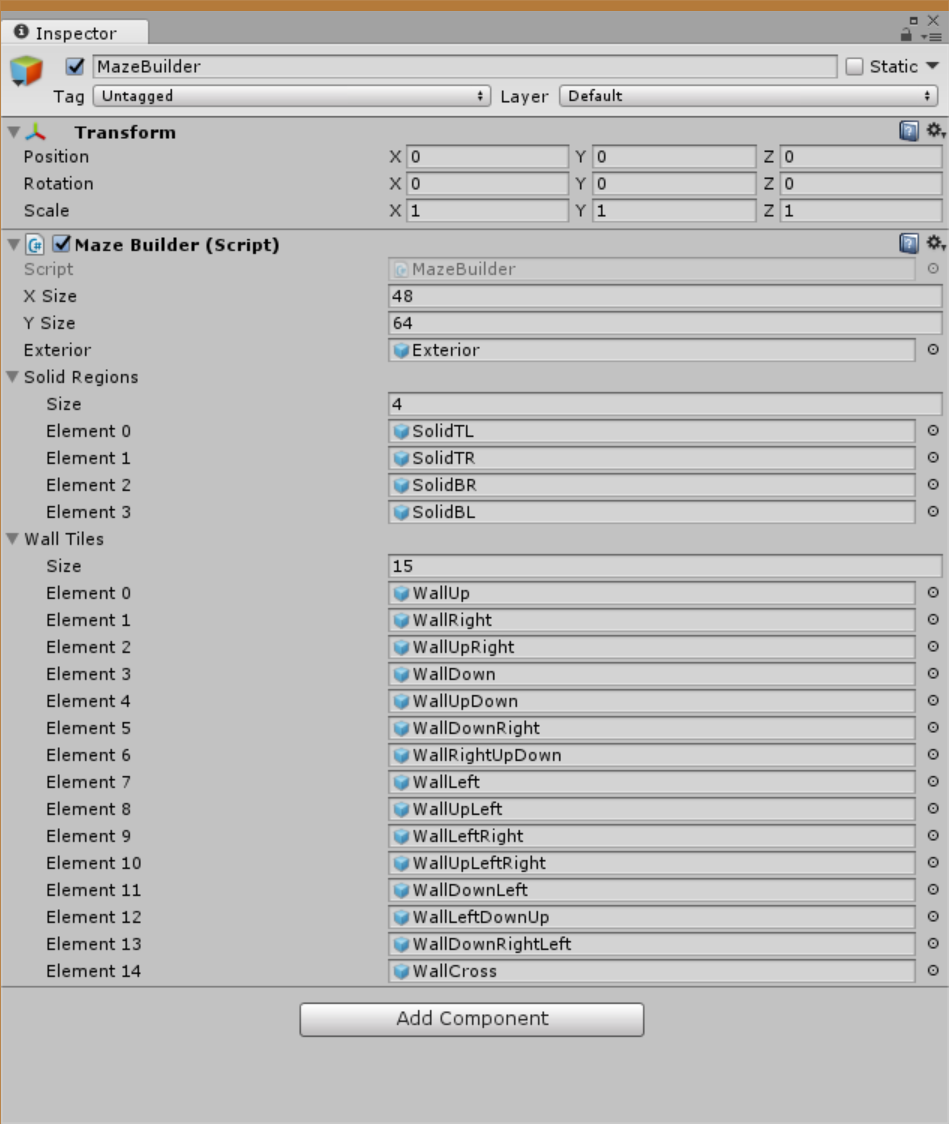
\includegraphics[width=6in]{MazeBuilderSettings.png}
  \caption{Wall Segments Imported into Unity}
  \label{fig:maze-builder-settings}
\end{figure}

First, we shall modify the script to fill the space with the exterior tile.

\begin{task}
Add the lines:
\begin{verbatim}
Instantiate(exterior, new Vector3(x, y, 10),
              Quaternion.identity, transform);
\end{verbatim}
just before the
\begin{verbatim}
if (grid[x, y]) {
\end{verbatim}
line.
\end{task}

This will place the exterior tiles 10 units behind the maze (we want to put other tiles on top of them).  Compile and run the game to be sure the exterior tiles show up, and are covered by other tiles.

Next we shall place the solid regions in the right places.  In the basic maze we have now, that is not too hard.  We look at the grid array of boolean values, and we look up, down, left, and right, to see if there is wall in those directions.  For example, if there is wall up and left of a grid point, then the up-left solid region is needed. 


\begin{task}
Add the lines:
\begin{verbatim}
//instantiate solid regions
int directions = 0;

if ((y >= ySize - 1) || grid[x, y + 1]) {//up
    directions += 1;
}
if ((y <= 0) || grid[x, y - 1]) {//down
    directions += 4;
}
if ((x <= 0) || grid[x - 1, y]) {//left
    directions += 8;
}
if ((x >= xSize - 1) || grid[x + 1, y]) {//right
    directions += 2;
}
if ((directions & 9) == 9) {//up left
    Instantiate(solidRegions[0], new Vector3(x, y, 9),
  Quaternion.identity, transform);
    directions += 16;
}
if ((directions & 3) == 3) {//up right
    Instantiate(solidRegions[1], new Vector3(x, y, 9),
  Quaternion.identity, transform);
    directions += 32;
}
if ((directions & 6) == 6) {//down right
    Instantiate(solidRegions[2], new Vector3(x, y, 9),
  Quaternion.identity, transform);
    directions += 64;
}
if ((directions & 12) == 12) {//down left
    Instantiate(solidRegions[3], new Vector3(x, y, 9),
  Quaternion.identity, transform);
    directions += 128;
}
\end{verbatim}
just after the
\begin{verbatim}
if (grid[x, y]) {
\end{verbatim}
line.
\end{task}
This instantiates the solid region tiles 9 units behind the camera, so they are over top the exterior tiles, but behind any other tiles we add.  In addition, we set a ``directions'' variable to a numeric code that we use to choose these solid regions, and that we shall use to choose wall tiles next.

\begin{task}
Finally, remove the WallPrefab code, both the declaration and the instantiation lines that use it.  Replace it with the following code:
\begin{verbatim}
  //Find the correct wall tile
int wallTile = 4;//let default be vertical
int count = (directions & 16) / 16 + (directions & 32) / 32
    + (directions & 64) / 64 + (directions & 129) / 128;
if (count == 1) {
    if ((directions & 16) != 0) {
        wallTile = 8;//up and left
    } else if ((directions & 32) != 0) {
        wallTile = 2;//up and right
    } else if ((directions & 64) != 0) {
        wallTile = 5;//down and right
    } else if ((directions & 128) != 0) {
        wallTile = 11;//down and left
    }
} else if ((directions & 15) == 10) {//horizontal
    wallTile = 9;
} else if ((directions & 48) == 48) {//horizontal
    wallTile = 9;
} else if ((directions & 192) == 192) {//horizontal
    wallTile = 9;
}
//TODO more cases for more complex mazes


if (count != 4) {//count==4 means solid region, no wall
    Instantiate(wallTiles[wallTile], new Vector3(x, y, 0),
           Quaternion.identity, transform);
}
\end{verbatim}
\end{task}

This only works for the basic maze, and in fact, is still not perfect: look at the corners of the maze.  But we have come a long way.  Compile and run and check that the maze looks like Figure \ref{fig:better-walls}.

\begin{figure}[h]
  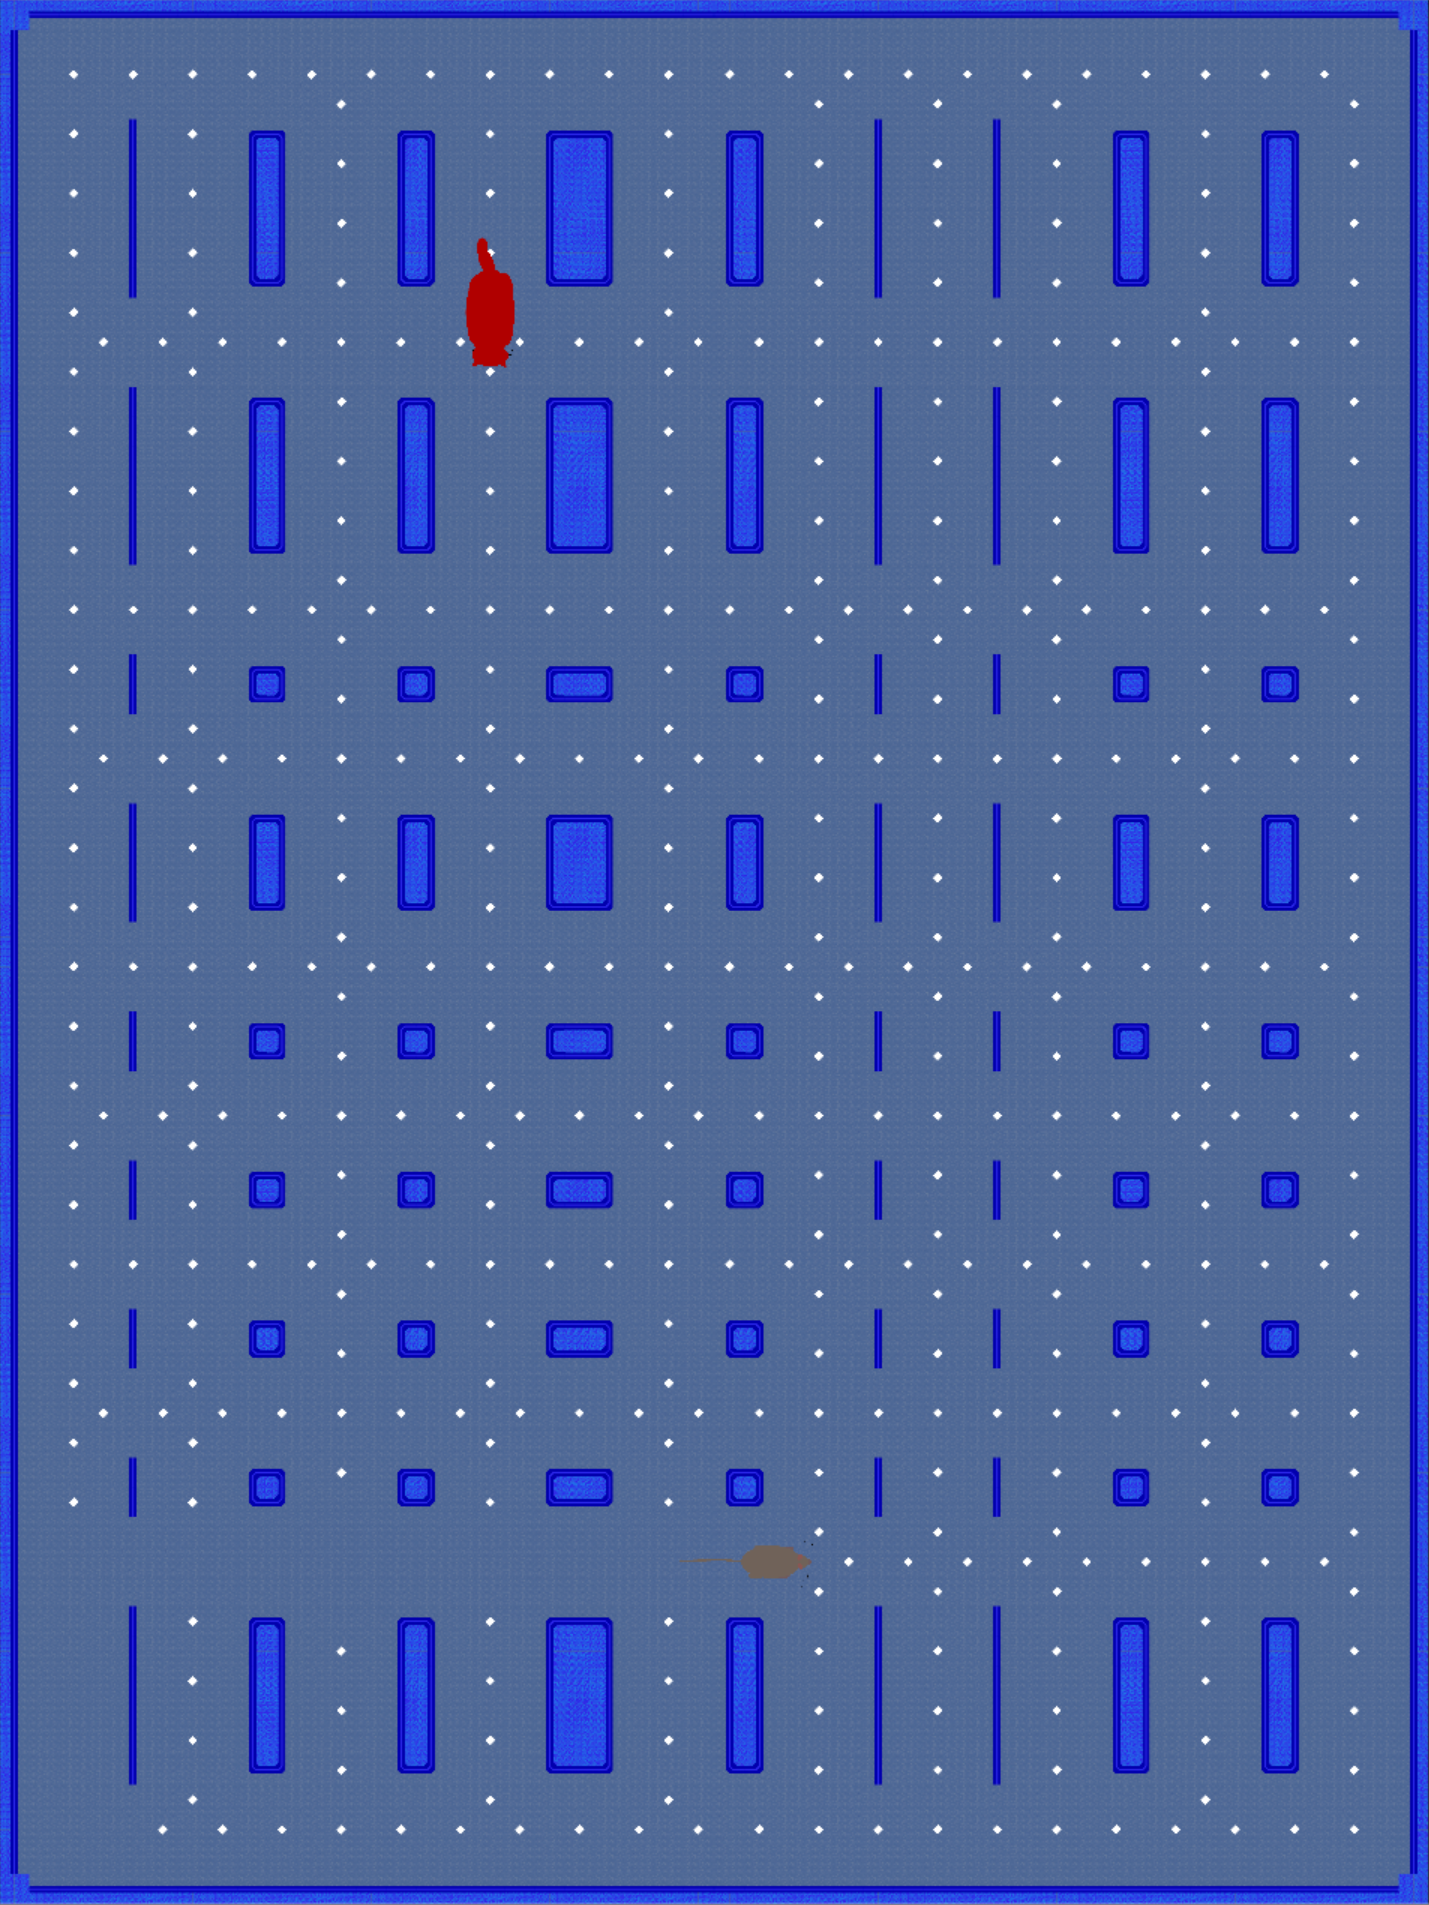
\includegraphics[width=3in]{BetterWalls.png}
  \caption{Walls Look Much Better}
  \label{fig:better-walls}
\end{figure}

For reference, here is what the MazeBuilder code looks like at this stage:

\begin{verbatim}
using System.Collections;
using System.Collections.Generic;
using UnityEngine;

public class MazeBuilder : MonoBehaviour {
    public int xSize = 48;
    public int ySize = 64;

    public GameObject exterior;
    public GameObject[] solidRegions;
    public GameObject[] wallTiles;

    private bool[,] grid;

    // Use this for initialization
    void Start() {
        Initialize();
        BasicMaze(10, 10);
        Draw();
    }

    // Update is called once per frame
    void Update() {

    }

    public void Initialize() {
        grid = new bool[xSize, ySize];
        for (int x = 0; x < xSize; x++) {
            for (int y = 0; y < ySize; y++) {
                grid[x, y] = true;
            }
        }
    }

    public void BasicMaze(int m, int n) {
        CarveRow(2);
        CarveRow(ySize - 3);
        CarveColumn(2);
        CarveColumn(xSize - 3);


        int[] RowWallWidth = new int[m - 1];
        for (int i = 0; i < m - 1; i++) {
            RowWallWidth[i] = 1;
        }
        for (int i = 0; i < ySize - 2 - 4 * m; i++) {
            int j = Random.Range(0, m - 1);
            RowWallWidth[j]++;
        }
        int r = 5;
        for (int i = 0; i < m - 2; i++) {
            r += RowWallWidth[i];
            CarveRow(r);
            r += 3;
        }

        int[] ColWallWidth = new int[n - 1];
        for (int i = 0; i < n - 1; i++) {
            ColWallWidth[i] = 1;
        }
        for (int i = 0; i < xSize - 2 - 4 * n; i++) {
            int j = Random.Range(0, n - 1);
            ColWallWidth[j]++;
        }
        int c = 5;
        for (int i = 0; i < n - 2; i++) {
            c += ColWallWidth[i];
            CarveColumn(c);
            c += 3;
        }
    }

    public void CarveRow(int y) {
        for (int x = 1; x <= xSize - 2; x++) {
            for (int j = y - 1; j <= y + 1; j++) {
                grid[x, j] = false;
            }
        }
    }

    public void CarveColumn(int x) {
        for (int y = 1; y <= ySize - 2; y++) {
            for (int j = x - 1; j <= x + 1; j++) {
                grid[j, y] = false;
            }
        }
    }

    public void Draw() {
        for (int x = 0; x < xSize; x++) {
            for (int y = 0; y < ySize; y++) {
                Instantiate(exterior, new Vector3(x, y, 10),
                      Quaternion.identity, transform);
                if (grid[x, y]) {


                    //instantiate solid regions
                    int directions = 0;

                    if ((y >= ySize - 1) || grid[x, y + 1]) {//up
                        directions += 1;
                    }
                    if ((y <= 0) || grid[x, y - 1]) {//down
                        directions += 4;
                    }
                    if ((x <= 0) || grid[x - 1, y]) {//left
                        directions += 8;
                    }
                    if ((x >= xSize - 1) || grid[x + 1, y]) {//right
                        directions += 2;
                    }
                    if ((directions & 9) == 9) {//up left
                        Instantiate(solidRegions[0], new Vector3(x, y, 9),
                      Quaternion.identity, transform);
                        directions += 16;
                    }
                    if ((directions & 3) == 3) {//up right
                        Instantiate(solidRegions[1], new Vector3(x, y, 9),
                      Quaternion.identity, transform);
                        directions += 32;
                    }
                    if ((directions & 6) == 6) {//down right
                        Instantiate(solidRegions[2], new Vector3(x, y, 9),
                      Quaternion.identity, transform);
                        directions += 64;
                    }
                    if ((directions & 12) == 12) {//down left
                        Instantiate(solidRegions[3], new Vector3(x, y, 9),
                      Quaternion.identity, transform);
                        directions += 128;
                    }

                    //Find the correct wall tile
                    int wallTile = 4;//let default be vertical
                    int count = (directions & 16) / 16 + (directions & 32) / 32
                        + (directions & 64) / 64 + (directions & 129) / 128;
                    if (count == 1) {
                        if ((directions & 16) != 0) {
                            wallTile = 8;//up and left
                        } else if ((directions & 32) != 0) {
                            wallTile = 2;//up and right
                        } else if ((directions & 64) != 0) {
                            wallTile = 5;//down and right
                        } else if ((directions & 128) != 0) {
                            wallTile = 11;//down and left
                        }
                    } else if ((directions & 15) == 10) {//horizontal
                        wallTile = 9;
                    } else if ((directions & 48) == 48) {//horizontal
                        wallTile = 9;
                    } else if ((directions & 192) == 192) {//horizontal
                        wallTile = 9;
                    }
                    //TODO more cases for more complex mazes


                    if (count != 4) {//count==4 means solid region, no wall
                        Instantiate(wallTiles[wallTile], new Vector3(x, y, 0),
                               Quaternion.identity, transform);
                    }
                }
            }
        }
    }

    public bool IsPlayerSpace(int x, int y) {
        if (x - 1 < 0 || y - 1 < 0) {
            return false;
        }
        if (x + 1 >= xSize || y + 1 >= ySize) {
            return false;
        }
        for (int i = x - 1; i <= x + 1; i++) {
            for (int j = y - 1; j <= y + 1; j++) {
                if (grid[i, j]) {
                    return false;
                }
            }
        }
        return true;
    }

}
\end{verbatim}

\chapter{Refactoring the Code}

\section{What is Refactoring?}

\section{Common Refactoring Operations}

\section{Make the Maze Less Boring}

In this section, we join some of the wall pieces together to make the maze more interesting.

\section{Improving the Mouse Animation}
The mouse currently faces to the right no matter which way it moves.  It also stays in the basic MouseIdle animation whether it is moving or not.  We now fix these issues.  First, we add a new MouseRun animation based on the MouseIdle animation, but with the feet moving.  

\subsection{Add a Run Animation}

\subsection{Set Up the Animator}

\subsection{Set up the Transitions}


\subsection{Modify the PlayerController Script}


\section{Improving the Cat Animation}
\begin{exercise}
Following the procedures of the last section, make the cat point in the direction it moves and stop "walking" when it is not moving.
\end{exercise}

\chapter{Unity Sound Framework}


\section{Installing Audacity}

\section{Bringing the Cats and Mouse to Life}
\section{Game Music}


\chapter[Framing the Game]{Framing the Game: Attract Mode and Game States}
\section{Discrete Finite Automata}
\cite{CSRL01}

\section{Scenes in Unity}
\section{Additional Game States}

\chapter{Options and Saving State}

\chapter{Video Playback}
\section{Installing Blender}
\section{Blender Crash Course}
\section{Blender Animation}
\section{Making a Cutscene}
\section{Demo Recording Framework Design}
Considerations: record frames as images, or record inputs? Latter is more flexible, can change ``view'' of the game for example (matters more in a 3D game), and takes less disk space, but Former is guaranteed to be ``WYSIWYG''.

\section{Demo Recording Framework Implementation}
\section[Recording Demos]{Recording Demos to Package with the Game} 

%%%%%%%%%%%%%%%% APPENDIX %%%%%%%%%%%%%%%%%
\appendix
\chapter[Selected Solutions]{Selected Solutions to Exercises}

\begin{figure}[h]
  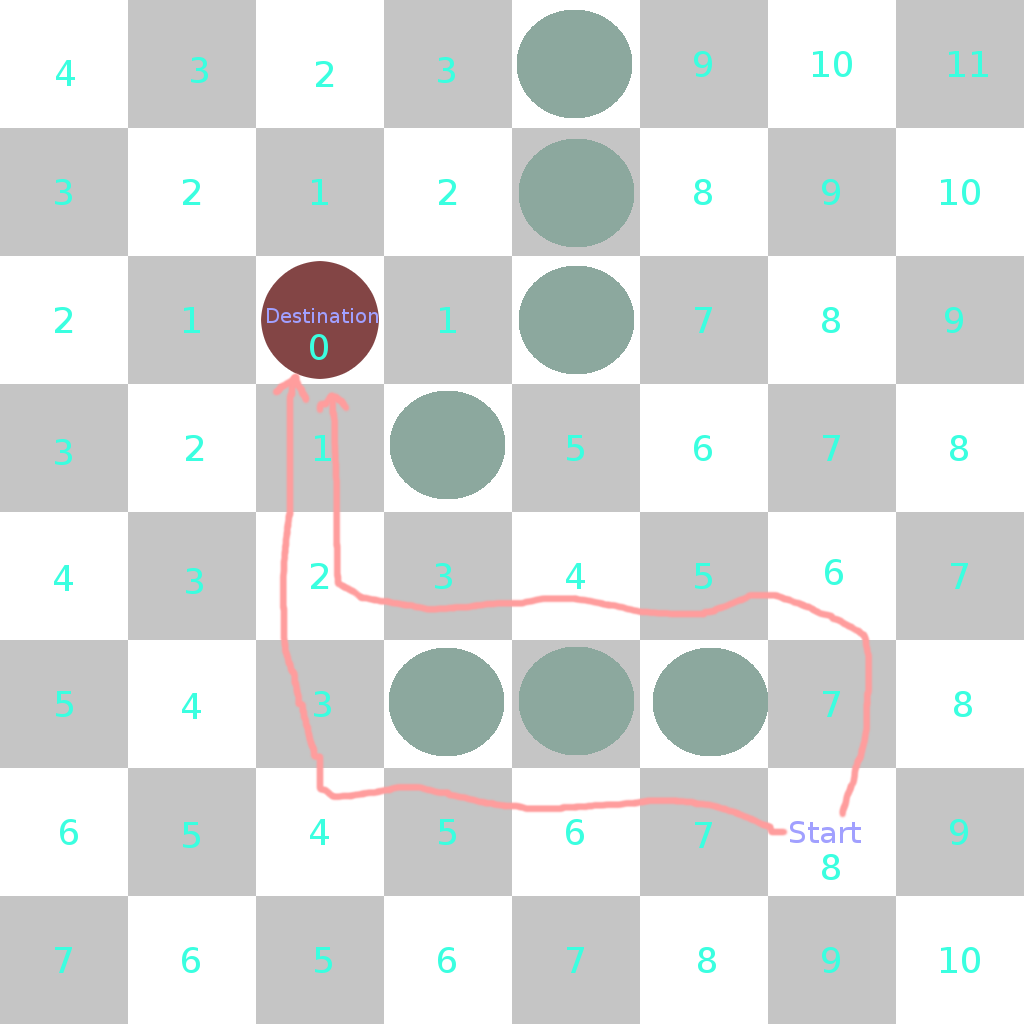
\includegraphics[width=3in]{CheckerboardSolution.png}
  \caption{There are two shortest paths from the start to the destination.}
  \label{fig:checkerboard-solution}
\end{figure}

\chapter{Installing Firefox and Acrobat Reader}

\section{Installing Firefox}

\section{Installing Acrobat Reader}

%%%%%%%%%%%%%%% END DOCUMENT %%%%%%%%%%%%%%%
\backmatter
\bibliographystyle{amsalpha}
\bibliography{master}
\printindex

\end{document}